\NeedsTeXFormat{LaTeX2e}[2005/12/01]
%%    2009/03/12 v1.0 GAUBM Vorlage f�r Aschlussarbeiten Physik
%% Template fuer Bachelor- und Masterarbeiten
%% an der Fakultaet fuer Physik (c) Thomas Pruschke der GA Universit�t
%% Verbesserungsvorschlaege bitte an pruschke@theorie.physik.uni-goettingen.de
%%
%% Benoetigte Pakete: datenumber
%%

%%%%%%%%%%%%%%%%%%%%%%%%%%%%%%%%%%%%%%%%%%%%%%%%%%%%%%%%%%%%%%%%%%%%%%
%%%%%%%%%% Bitte vor dem Veraendern diese Datei umbenennen! %%%%%%%%%%
%%%%%%%%%%%%%%%%%%%%%%%%%%%%%%%%%%%%%%%%%%%%%%%%%%%%%%%%%%%%%%%%%%%%%%

%% scrbook - Ersatz f�r LaTeX book Klasse aus dem KOMA Script
%% Moegliche Optionen: diejenigen der Klasse scrbook ausser titlepage

%% deutsche Arbeit:
\documentclass[bachelor,       %% Typ der Arbeit: bachelor oder master
               twoside,        %% zweiseitiges Layout
               BCOR10mm,       %% Bindekorrektur 10 mm
%               liststotoc,nomtotoc,bibtotoc, %% Aufnahme der div. Verzeichnisse
                                              %% ins Inhaltsverzeichnis
%               english,ngerman, %% Alternativspr. Englisch, Dokumentspr. Deutsch
               ngerman,english  %% Alternativspr. Deutsch, Dokumentspr. Englisch
%               final,          %% Endversion; draft fuer schnelles Kompilieren
               ]{GAUBM}

\usepackage{setspace}  %% Zur Setzung des Zeilenabstandes
\usepackage{babel}     %% Sprachen-Unterstuetzung
\usepackage{calc}      %% ermoeglicht Rechnen mit Laengen und Zaehlern
\usepackage[T1]{fontenc}       %% Unterstutzung von Umlauten etc.
\usepackage[latin1]{inputenc}  %% 
%% in aktuellem Linux & MacOS X wird standardmaessig UTF8 kodiert!
%\usepackage[utf8]{inputenc}    %% Wenn latin1 nicht geht ...

\usepackage{amsmath,amssymb} %% zusaetzliche Mathe-Symbole

\usepackage{lmodern} %% type1-taugliche CM-Schrift als Variante zur
                     %% "normalen" EC-Schrift
%% Paket fuer bibtex-Datenbanken
\usepackage[comma,numbers,sort&compress]{natbib}
\bibliographystyle{plainnat}

\newcommand{\tabheadfont}[1]{\textbf{#1}} %% Tabellenkopf in Fett
\usepackage{booktabs}                      %% Befehle fuer besseres Tabellenlayout
\usepackage{longtable}                     %% umbrechbare Tabellen
\usepackage{array}                         %% zusaetzliche Spaltenoptionen

%% umfangreiche Pakete fuer Symbole wie \micro, \ohm, \degree, \celsius etc.
\usepackage{textcomp,gensymb}

%\usepackage{SIunits} %% Korrektes Setzen von Einheiten
\usepackage{units}   %% Variante fuer Einheiten

%% Hyperlinks im Dokument; muss als eines der letzten Pakete geladen werden
\usepackage[pdfstartview=FitH,      % Oeffnen mit fit width
            breaklinks=true,        % Umbrueche in Links, nur bei pdflatex default
            bookmarksopen=true,     % aufgeklappte Bookmarks
            bookmarksnumbered=true  % Kapitelnummerierung in bookmarks
            ]{hyperref}

%% Weiter benoetigte Pakete: datenumber
%% Falls dieses Paket nicht in der Installation vorhanden ist,
%% kann es von der Seite mit diesem Template heruntergeladen werden
%% und in einem LaTeX bekanntem Verzeichnis installiert werden (notfalls
%% dem Verzeichnis mit der Arbeit).

%%%%%%%%%%%%%%%%%%%%%%%%%%%%%%%%%%%%%%%%%%%%%%%%%%%%%%%%%
%%%%%%%%%%%%%% EIGENE VER�NDERUNGEN:#####################
%% Bra-Ket Notation: \bracket{||} oder \bra{}
\usepackage{caption}
\usepackage{subcaption}

\usepackage{braket}

\usepackage{cleveref}
\usepackage{bm}
\usepackage{algpseudocode}
\usepackage{algorithmicx}

\newcommand{\vect}[1]{\bm{#1}}
\renewcommand{\d}[1]{\ensuremath{\operatorname{d}\!{#1}}}
%%########################################################
%%%%%%%%%%%%%%%%%%%%%%%%%%%%%%%%%%%%%%%%%%%%%%%%%%%%%%%%%%

\begin{document}
%%
%%                   Ab hier muessen die Anpassungen geschehen
%%
%% Hier den eigenen Namen einsetzen
\ThesisAuthor{Eric}{Bertok}
%% Hier den Geburtsort einsetzen
\PlaceOfBirth{Kassel}
%% Titel Arbeit. Das erste Argument ist der deutsche, das zweite der
%% englische Titel.
\ThesisTitle{Hier steht das Thema der Arbeit in deutsch}{Here comes the title of the thesis in english}
%% Erst- und Zweitgutacher/in
%% Ist der/die Betreuer/in nicht identisch mit dem/r Erstgutachter/in,
%% muss diese/r als optionales Argument angegeben werden.
\FirstReferee[Dr.\ \ldots]{Prof.\ Dr.\ Kehrein}
\Institute{Institut f\"ur Theoretische Physik}
\SecondReferee{Prof.\ Dr.\ Kree}
%% Beginn und Ende des Anfertigungszeitraumes
\ThesisBegin{1}{4}{2009}
\ThesisEnd{15}{7}{2009}
%% DO NOT TOUCH THESE LINES!!!!
\frontmatter
\maketitle
\cleardoublepage
%% Zusammenfassung. Falls nicht gewuenscht, bitte auskommentieren.
\begin{abstract}
  Here the key results of the thesis can be presented in about
  half a page.
  \bigskip\par
  \textbf{Keywords:} Physics, Bachelor thesis
  \end{abstract}
%% So laesst sich in die andere Sprache umschalten (Englisch bzw. Deutsch)
\begin{otherlanguage}{ngerman}
\begin{abstract}
  Hier werden auf einer halben Seite die Kernaussagen der Arbeit
  zusammengefasst.
%% Optional: Stichwoerter. Wenn nicht gewuenscht, koennen die beiden
%% folgenden Zeilen geloescht werden
  \bigskip\par
  \textbf{Stichw�rter:} Physik, Bachelorarbeit

\end{abstract}
\end{otherlanguage}

%% Ende des Vorspanns
\cleardoublepage
%% Ab hier 1 1/2 facher Zeilenabstand (durch setspace-Paket)
\onehalfspacing
%% Erzeugt Inhaltsverzeichnis
\tableofcontents

%% Hier kann man seine Bezeichnungsweisen erklaeren. Falls nicht
%% benoetigt, bis einschliesslich \end{nomenclature} auskommentieren
\begin{nomenclature}
%% Fuer die Berechnung der Spaltenbreiten muss \usepackage{calc}
%% geladen sein!
\section*{Lateinische Buchstaben}
\noindent
\begin{longtable}[l]{p{0.2\textwidth}p{0.7\textwidth-6\tabcolsep}p{0.1\textwidth}}
  \tabheadfont{Variable}&\tabheadfont{Bedeutung}&\tabheadfont{Einheit}\\\midrule\endhead
  $A$ & Querschnittsfl"ache & $\unit{m^2}$\\
  $c$ & Geschwindigkeit & $\unitfrac{m}{s}$
\end{longtable}
\section*{Griechische Buchstaben}
\begin{longtable}[l]{p{0.2\textwidth}p{0.7\textwidth-6\tabcolsep}p{0.1\textwidth}}
  \tabheadfont{Variable}&\tabheadfont{Bedeutung}&\tabheadfont{Einheit}\\\midrule\endhead
  $\alpha$  & Winkel & $\unit{\degree}$; --\\
  $\varrho$ & Dichte & $\unitfrac{kg}{m^3}$
\end{longtable}
\section*{Indizes}
\begin{longtable}[l]{p{0.2\textwidth}p{0.8\textwidth-4\tabcolsep}}
  \tabheadfont{Index}&\tabheadfont{Bedeutung}\\\midrule\endhead
  m & Meridian\\
  $r$ & Radial
\end{longtable}
\section*{Abk"urzungen}
\begin{longtable}[l]{p{0.2\textwidth}p{0.8\textwidth-4\tabcolsep}}
  \tabheadfont{Abk"urzung}&\tabheadfont{Bedeutung}\\\midrule\endhead
  2D & zweidimensional\\
  3D & dreidimensional\\
  max & maximal
\end{longtable}
\end{nomenclature}
%% \listoftables und \listoffigures sollten nur bei genuegender Anzahl Tabellen
%% verwendet werden
%\listoffigures
%\listoftables

\mainmatter   %% Anfang Hauptteil

\chapter{Einleitung}
Diese Vorlage \verb!GAUBM!
f�r Bachelor- bzw.\ Masterarbeiten ist eine �berarbeitung der
Vorlage von Simon Dreher f�r Abschlu�arbeiten am
Institut f�r Mikrosystemtechnologie (IMTEK)
an der Universit�t Freiburg. Die eigentliche Datei mit der Klassendefinition
ist \verb!GAUBN.cls!, die Sie zusammen mit dieser Datei erhalten haben. Weitere
Dateien sind \verb!datenumber.sty! und die zugeh�rigen Sprachdefinitionen
\verb!\datenumber*.ldf!. Im Verzeichnis \verb!figures! finden sich die
von der Klasse ben�tigten Logos (Universit�t und Physik) sowie Beispielbilder
f�r die �bersetzung dieser Beispieldatei (\verb!bthesis.tex!).
Sie k�nnen diese Datei als Vorlage f�r Ihre Arbeit nutzen und entsprechend
modifizieren. Bitte denken Sie daran, sie vorher unter einem eigenen Namen
abzuspeichern.
Um die Datei anzupassen, gehen Sie wie folgt vor:

Bei den Parametern zu \verb!\documentclass[...]{GAUBM}! in der Pr�ambel
kann man durch Umschalten
zwischen \verb!english,ngerman! und \verb!ngerman,english! eine
deutsche Arbeit (erste Variante) mit Englisch als Alternativsprache bzw.\ eine
englische Arbeit (zweite Variante) mit deutsch als Alternativsprache
w�hlen. Im laufenden Text kann man mit 
\begin{verbatim}
\begin{otherlanguage}{english/ngerman}
...
\end{otherlanguage}
\end{verbatim}
zur alternativen Sprache wechseln.

Nach \verb!\begin{document}! m�ssen zuerst ein paar Befehle mit
Information �ber die Arbeit aufgerufen werden:
\begin{enumerate}
\item \verb!\ThesisAuthor{Vorname}{Nachname}!: Die Argumente sind der
Vorname und Nachname der Autorin bzw.\ des Autors der Arbeit.
\item \verb!\PlaceOfBirth{Wohnort}!: Der Geburtsort der Autorin bzw.\ des Autors.
\item \verb!\ThesisTitle{Deutscher Titel}{English title}!: Der deutsche und englische Titel der Arbeit gem�� Antrag.
\item \verb!\Institute{Institut}!: Das Institut, an dem die Arbeit angefertigt wurde.
\item \verb!\FirstReferee[Betreuer/in]{Erste/r Gutachter/in}!: Voller Titel
und Name des/r Erstgutachter/in. Ist der Betreuer der Arbeit \emph{nicht}
identisch mit dem/r Erstgutachter/in, so mu� der volle Titel und der Name
des/r Betreuer/in als optionales Argument in eckigen Klammern erscheinen.
\item \verb!\SecondReferee{Zweite/r Gutachter/in}!: Voller Titel
und Name des/r Zweitgutachter/in.
\item \verb!\ThesisBegin{Tag}{Monat}{Jahr}!: Datum des Beginns der Anfertigung
der Arbeit gem�� Antrag.
\item \verb!\ThesisEnd{Tag}{Monat}{Jahr}!: Datum der Fertigstellung der Arbeit.
\item Optional kann mit
\begin{verbatim} 
\begin{abstract}
...
\end{abstract}
\end{verbatim}
eine maximal eine halbe Seite lange Zusammenfassung eingef�gt werden.

Falls man die Zusammenfassung in der alternativen Sprache verfassen m�chte,
dann geht das mit der Befehlsfolge
\begin{verbatim} 
\begin{otherlanguage}{english/ngerman}
\begin{abstract}
...
\end{abstract}
\end{otherlanguage}
\end{verbatim}
\end{enumerate}

\chapter{Grundlagen}
In diesem Kapitel werden die theoretischen Grundlagen erl�utert.

Wichtige Gleichungen, die in der Arbeit h�ufiger zitiert werden,
sollten eine Gleichungsnummer erhalten.
\begin{equation}
  \label{eq:pythagoras}
  a^2+b^2=c^2
\end{equation}
Zum Beispiel wird in Gleichung~\ref{eq:pythagoras} der Satz des Pythagoras
angegeben.

Gerade im Bereich der Grundlagen wird viel Literatur zitiert, z.B.\
\cite{Menz97}. Falls
mehrere Literaturzitate auf einmal zitiert werden, ist folgendes
z.B.\ m�glich \cite{Horn90,DINEN6232,Menz97,Knuth84}.

\section{Unterkapitel Gliederungsebene 2}
Hier sollte etwas Text stehen.
\subsection{Unterkapitel Gliederungsebene 3}
Noch ein paar Beispiele zu Abbildungen und Tabellen:

Abbildung~\ref{fig:bildplatzhalter} verdeutlicht \dots

Wie die Abb.~\ref{fig:bildplatzhalter} und
Tab.~\ref{tab:tabellenplatzhalter} verdeutlichen \dots

\begin{figure}
  \centering
  
\includegraphics[width=0.5\linewidth]{figures/bild}
  \caption{Bildbeschreibung}
  \label{fig:bildplatzhalter}
\end{figure}

Text\dots
\begin{table}
  \centering
  \begin{tabular}{llll}
    \toprule
    $A$-Wert&$B$-Wert&$C$-Wert&$D$-Wert\\
    \midrule
    aaaaaa&bbbbbbb&cccccc&ddddddd\\
    aaaaaa&bbbbbbb&cccccc&ddddddd\\
    \bottomrule
  \end{tabular}
  \caption{Tabellenbeschreibung}
  \label{tab:tabellenplatzhalter}
\end{table}

Text\dots

\chapter{``Lab course''}
\section{Theoretical foundation and numerical methods}
\subsection{Introduction, exact diagonalization}
In what follows, we are interested in a one-dimensional XXZ Heisenberg chain with next-nearest neighbour coupling. As such, we consider the following Hamiltonian:
\begin{align}
    H(J,\mu)&=H_1(J,\mu)+\lambda H_2(J,\mu),\\
    H_n(J,\mu)&=J \sum_{i=1}^{N}\left[\frac{1}{2}\left( S_i^+ S_{i+n}^- + S_i^- S_{i+n}^+ \right)+\mu S_i^z S_{i+n}^z\right],
    \label{eq:XXZham}
\end{align}
where the spins are labeled $i=1,\dots,N$ and $J$ is the interaction constant. The scalar product for the spin operators $\mathbf{S}_i\cdot\mathbf{S}_{i+n}$ has been decomposed into creation-annihilation operators $S^\pm=S^x \pm i S^y$ while  $\mu$ introduces an anisotropy for the z-direction compared to the x and y directions.
Finally, $\lambda$ is a parameter controlling the strength of the next-nearest neighbor (NNN) interactions cf. \cite[4ff.]{xxz_springer}.\\
First, would like to numerically compute the time evolution of such a system by means of exact diagonalization.
\subsection{Block diagonalization}
In the following section, we follow closely the techniques and notation from \cite[55ff.]{sand11}.
The states are denoted as $\ket{S_0^z,S_1^z,\dots,S_{N-1}}$, where the subscript $i=0,\dots,N-1$ refers to the site $i$ of our one-dimensional chain. A particular state is abridgedly labeled by arrows, e.g.
$\ket{\uparrow\downarrow\uparrow\downarrow\dots}$.
Furthermore, periodic boundary conditions, which add additional symmetries, are assumed ($i=N-1+n\equiv n-1\label{eq:periodic}$).
Exact diagonalization allows for total knowledge of the properties of a finite system by choosing a basis, setting up a Hamiltonian and diagonalizing it numerically. While theoretically applicable to any system size, this method is limited to around 30 spins, as the computational cost for diagonalization is $\propto 8^\text{dim. of basis}$[citation needed.] and the spin basis above grows like $2^N$ without utilizing symmetries.
Symmetries can be used to transform the Hamiltonian matrix into block-diagonal form cf. \cite[56]{sand11} with each block belonging to states with a conserved quantum number, thereby reducing the basis dimension. In this first chapter, only the conservation of z-component of the total spin ($\hat{=}$ total magnetization) $m_z=\sum_{i=0}^{N-1} S_i^z$ is used:\\
It is easy to verify, using the usual commutation relations for the spin operators [citation needed] that
\begin{align}
    [S_i^z,H]&=\frac{1}{2}(A_1+A_2),\\
    A_n&=S_i^+ S_{i+n}^- -S_i^- S_{i+n}^+ -S_{i-n}^+ S_i^- +S_{i-n}^- S_i^+.
    \label{eq:comm}
\end{align}
By using the periodic boundary conditions it follows that
\begin{align}
    \sum_{i=0}^{N-1}A_n=\sum_{i=0}^{N-1}\left( S_i^+ S_{i+n}^- -S_i^- S_{i+n}^+ \right)-\underbrace{\sum_{i=n}^{N-1+n}}_{\equiv\sum_{i=0}^{N-1}}\left( S_i^+ S_{i+n}^- -S_i^- S_{i+n}^+ \right)=0,
    \label{eq:Ancomm}
\end{align}
and therefore
\begin{align}
    \left[H,m_z\right]=0,
    \label{eq:totalmagcomm}
\end{align}
meaning that $m_z$ is a conserved quantity. By constructing a basis with fixed magnetization, blocks of size $M\times M$ with the same $m_z$ can be considered independently. $M$ is the fixed magnetization basis dimension: \cite[60]{sand11}

\begin{align}
    M=\frac{N!}{n_{\uparrow}!~  n_{\downarrow}!}.     \label{eq:fixedmagdim}
\end{align}

\subsection{Bit representation}
As Spin-$1/2$ partlicles only have two possible states $(\uparrow \& \downarrow)$, they can be elegantly represented in a computer via the bits ``1'' and ``0''.
More precisely, A lattice state $\ket{S_0^z,S_1^z,\dots,S_{N-1}}$ is represented as the bit representation of an unsigned integer, with the first bit denoted by the index 0. \cite[59]{sand11}, e.g. $\ket{\uparrow\downarrow\downarrow\uparrow}\hat{=} ~1001~ \dot{=}~9$. Symmetries that will come in later, like spin translation or rotation manifest themselves as operations on these bit representations.\\

\subsection{Construction of the fixed magnetization basis}
A basis list of states having the same magnetization $m_z$ is found by iterating over all integers $s$ from the $2^n$ dimensional basis and counting the amount of ``1'' bits $n_\uparrow$, checking whether they amount to the target magnetization $m_z$=$n_\uparrow-N/2$.\\
With $s[i]$ labeling the $i$'th bit, starting from 0, the following pseudocode is used to obtain an ordered list of basis states $s_a$:

\begin{algorithmic}
    \State $a=0$
    \ForAll{$s=0..2^N-1$}
    \If{$\sum_i s[i]=n_\uparrow$}
        \State$ a \gets a+1$
        \State$s_a \gets s$
        \EndIf
    \EndFor
    \State $M\gets a$
\end{algorithmic}\label{pseudo:basismag}
$M$ is the basis dimension. Thus, in terms of $M$-tuples, a natural basis is given by all vectors 
\begin{align}
    \hat{e}_a=(0,\dots,0,\underbrace{1}_{c_a},0,\dots,0)^T, a=1..M,     \label{eq:basismag}
\end{align}
each representing the corresponding integer state $s_a$.

\subsection{Construction of the Hamilton matrix}
The Hamiltonian (\ref{eq:XXZham}) is translated into a matrix for the fixed magnetization basis cf. \cite[60f.]{sand11}.
The diagonal terms are $\braket{a|S_i^z S_{i+n}^z|a}=\pm1/4~\mu$ ,since the $i$'th and $i+n$'th spin are either equal or different.
The off-diagonal terms $\left( S_i^+ S_{i+n}^- + S_i^- S_{i+n}^+ \right)$ flip the bits $i$ and $i+n$ $(0\leftrightarrow1)$ and amount to zero otherwise.
A bisectional search [Pseudocode?] is used to find position $b$ of the flipped state $s^*$, giving a matrix element contribution of $\braket{b|( S_i^+ S_{i+n}^- + S_i^- S_{i+n}^+ )|a}=+1/2$.
In pseudocode, the matrix belonging to the NNN Hamiltonian ($n=1,2$) is constructed as follows:
\begin{algorithmic}
    \For{$a=1..M$}
    \For{$n=1,2$}
    \State $j=(i+n)\mod N$
    \If{$a[i]=a[j]$}
    \State $H(a,a)\gets H(a,a)+\frac{1}{4}~\mu$
    \Else
    \State $H(a,a)\gets H(a,a)-\frac{1}{4}~\mu$
    \State $s^*=\text{flipstate}(a)$
    \State $b\gets$ findstate($s^*$)
    \State $H(a,b)=\frac{1}{2}$
    \EndIf
    \EndFor
    \EndFor
\end{algorithmic}

\subsection{Diagonalization and time evolution}
The Armadillo package \cite{Armadillo} is used for matrix diagonalization and vector operations.
After setting up the Hamilton matrix, the eigenvectors and eigenvalues are computed. Each eigenstate $\ket{\lambda}$ is a superposition of the natural spin states $\ket{a}=\ket{\uparrow\downarrow\uparrow\uparrow\dots\downarrow}$ , which themselves are represented by the bits of an integer. The vectors $\mathbf{c}$, which represent the states and have components $c_a$, are to be transformed into the eigenbasis. A general initial state $\ket\psi$ is decomposed in the eigenbasis as follows:
\begin{align}
    H\ket{\psi}&=\sum_a\sum_b \ket{a}\underbrace{\braket{a|H|b}}_{H_{ab}} \underbrace{\braket{b|\psi}}_{c_b}=\sum_a\sum_b\sum_\lambda  \ket{a}\braket{a|\lambda|\lambda}\braket{\lambda|b}\braket{b|\psi}\nonumber\\
    &=\sum_\lambda \lambda\ket{\lambda}\underbrace{\braket{\lambda|\psi}}_{c_\lambda},
    \label{eq:eigendecomposition}
\end{align}
where $c_\lambda$ are the components of the vector $\mathbf{c}$ in the eigenbasis and $\lambda$ are the eigenvalues (energies). The matrix elements and column vectors are what we actually work with. The natural spin states remain untouched.\\
We would now like to compute the time evolution of the system, which is done in the eigenbasis. Utilizing the time evolution operator $U(t)=e^{-iHt}$ it holds that
\begin{align}
    e^{-iHt}\ket{\psi}=e^{-iHt}\sum_\lambda c_\lambda\ket{\lambda}=\sum_\lambda \underbrace{e^{-i\lambda t}c_\lambda}_{c_\lambda (t)}\ket{\lambda}.
    \label{eq:timeevolution}
\end{align}
\subsection{Measurements and observables}
In light of the probabilistic nature of quantum mechanics, we are interested in measuring the expectation value of an observable $\braket{O}$.
Another important quantity later on will be the Loschmidt echo $M$ \cite{loschmidt_scolarpedia}, which is generally defined as
\begin{align}
    M(t)=\left|\braket{\psi_0|e^{iH_2 t} e^{-iH_1 t}|\psi_0}\right|.
    \label{eq:loschmidt_general}
\end{align}
For the first test of the time evolution, the special case with $H_2=0$ is considered, which makes $M$ a measure of similarity of the time evolved state with the initial state.\\
The Loschmidt echo is most easily computed in the eigenbasis, since it is not dependent on the basis used, and the eigenbasis is utilized for time evolution anyway.
In the matrix picture:
\begin{align}
    \braket{\psi_0|e^{-iHt}|\psi_0}=\sum_\lambda\braket{\lambda|c_\lambda^* e^{-i\lambda t} c_\lambda|\lambda}=\sum_\lambda c_\lambda^*(0) c_\lambda(t)=\mathbf{c}^*(0)\cdot \mathbf{c}(t).
    \label{eq:loschmidt_initial}
\end{align}
For the expectation values of observables, the state vector has to be transformed back into the natural basis because access to the natural spin states is needed in order to evaluate the action of the operators.
For example, measurement of $\braket{S_i^z}$ is done as follows: For the state vector $\mathbf{c}$ in the natural basis, every state represented by each component like in \cref{eq:basismag} is iterated over and the spin state ($\hat{=}$ bit ) of the $i$'th component of the integer $s_a$ is read out.
The expectation value is then
\begin{align}
    \braket{S_i^z}_t=\sum_{a,b}c_a^*(t)\braket{a|S_i^z|b}c_a(t)=\sum_a |c_a(t)|^2 S_i^z,
    \label{eq:sz_i_exp}
\end{align}
since the operator $S_i^z$ is diagonal in the natural basis.
Analogously, the spin-spin correlation operator $S_i^z S_{i+n}^z$ is handled.
\section{Tests of the time evolution}
We would like to check, whether our time evolution as computed in the previous chapter gives the right results. For this reason, different tests are carried out and compared to theoretical predictions for certain special cases of the dynamics. 
\subsection{Short-time evolution}
The goal is to check, whether the computed time evolution is correct up to a small time $t$. 
We start from the Heisenberg equation of motion
\begin{align}
    \frac{\d O_H}{\d t}=i[H,O_H],
    \label{eq:heisenberg}
\end{align}
where $H$ is the Hamiltonian and
\begin{align}
    O_H(t)=e^{(iHt)}Oe^{(-iHt)}.
    \label{eq:heisenbergop}
\end{align}
The subscript $H$ is dropped in what follows. 
Using the Baker-Campbell-Hausdorff formula $\text{Ad}_{\exp {iHt}}=\exp{\text{ad}_{iHt}}$ and expanding to second order, we get
\begin{align}
    O(t)\approx O+i[H,O]t-\frac{1}{2}\left[H,[H,O]\right]t^2,~ ~O\equiv O(0).
    \label{eq:shorttime}
\end{align}
We want to consider the expectation value of the $i$th spin $\braket{S_i^z}$ for the total antiferromagnetic state 
\begin{align}
    \ket a=\ket{\uparrow\downarrow\uparrow\downarrow\dots\downarrow\uparrow}.
    \label{eq:totalantif}
\end{align}
As the Heisenberg equation also holds for expectation values of operators, our expansion reads
\begin{align}
    \braket{S_i^z}_t=\braket{S_i^z}_0+i\braket{[H,S_i^z]}t-\frac{1}{2}\braket{\left[ H,[H,S_i^z] \right]}t^2+\mathcal{O}(t^3).
    \label{eq:kurzexpansion}
\end{align}
From \cref{eq:comm} it is apparent that the linear term drops out, since all angular momentum eigenstates with different $S^z$ are orthogonal to each other. Following the same line of reasoning, and using $S^\pm S^\mp=\mathbf{S}^2-(S^z)^2\pm S^z$, one can show that 
\begin{align}
    \bra{\psi}\left[ H,[H,S_i^z] \right]\ket \psi =\bra \psi \left[ (S_{i-1}^+ S_{i-1}^- + S_{i+1}^+ S_{i+1}^-)S_i^z-S_i^+ S_i^- S_{i-1}^z-S_i^+ S_i^- S_{i+1}^z \right]\ket\psi \nonumber\\
    =\bra \psi \big[ \left( \mathbf{S}_{i-1}^2-(S_{i-1}^z)^2+S_{i-1}^z+\mathbf{S}_{i+1}^2-(S_{i+1}^z)^2+S_{i+1}^z \right)S_i^z\nonumber\\
    -\left( \mathbf{S}_i^2-(S_i^z)^2+S_i^z \right)\left( S_{i-1}^z+S_{i+1}^z \right) \big]\ket \psi.
    \label{eq:secondorderexp}
\end{align}
Evaluating this expression for the state given in \cref{eq:totalantif} results in the following approximation for the short-time evolution:
\begin{align}
    \braket{S_i^z}_t=\pm\frac{1}{2}\mp\frac{1}{2}t^2+\mathcal{O}(t^3),
    \label{eq:kurzzeit}
\end{align}
where the upper signs are to be used with a spin up as the initial $i$ state ($\ket{\dots\underbrace{\uparrow}_i\dots})$ and vice versa. 
In \cref{fig:kurzzeit}, the time evolution of $\braket{S_1^z}$ computed with the program is plotted for variable system sizes $N=2,4,6,8,10,12,14$ with $\mu=0$, $\lambda=0$ in \cref{eq:XXZham}. The dashed blue line is the short-time approximation \cref{eq:kurzzeit}, which correctly describes the short-time behaviour of the system. Furthermore, it can be shown that for an infinite system size, the expectation value of the spin can be expressed using the zeroth Bessel function [citation needed!]:
\begin{align}
    \braket{S_i^z}_t\big|_{N\rightarrow\infty}=\mp\frac{1}{2}J_0(2t),
    \label{eq:besselkurzzeit}
\end{align}
which is also shown in \cref{fig:kurzzeit}. As $N$ increases, the expectation value computed by the program matches this theoretical prediction longer and longer.
Overall, this is a clear indication that the time evolution computed by the program is correct.

\begin{figure}[]
    \centering
    % GNUPLOT: LaTeX picture with Postscript
\begingroup
  \makeatletter
  \providecommand\color[2][]{%
    \GenericError{(gnuplot) \space\space\space\@spaces}{%
      Package color not loaded in conjunction with
      terminal option `colourtext'%
    }{See the gnuplot documentation for explanation.%
    }{Either use 'blacktext' in gnuplot or load the package
      color.sty in LaTeX.}%
    \renewcommand\color[2][]{}%
  }%
  \providecommand\includegraphics[2][]{%
    \GenericError{(gnuplot) \space\space\space\@spaces}{%
      Package graphicx or graphics not loaded%
    }{See the gnuplot documentation for explanation.%
    }{The gnuplot epslatex terminal needs graphicx.sty or graphics.sty.}%
    \renewcommand\includegraphics[2][]{}%
  }%
  \providecommand\rotatebox[2]{#2}%
  \@ifundefined{ifGPcolor}{%
    \newif\ifGPcolor
    \GPcolortrue
  }{}%
  \@ifundefined{ifGPblacktext}{%
    \newif\ifGPblacktext
    \GPblacktexttrue
  }{}%
  % define a \g@addto@macro without @ in the name:
  \let\gplgaddtomacro\g@addto@macro
  % define empty templates for all commands taking text:
  \gdef\gplbacktext{}%
  \gdef\gplfronttext{}%
  \makeatother
  \ifGPblacktext
    % no textcolor at all
    \def\colorrgb#1{}%
    \def\colorgray#1{}%
  \else
    % gray or color?
    \ifGPcolor
      \def\colorrgb#1{\color[rgb]{#1}}%
      \def\colorgray#1{\color[gray]{#1}}%
      \expandafter\def\csname LTw\endcsname{\color{white}}%
      \expandafter\def\csname LTb\endcsname{\color{black}}%
      \expandafter\def\csname LTa\endcsname{\color{black}}%
      \expandafter\def\csname LT0\endcsname{\color[rgb]{1,0,0}}%
      \expandafter\def\csname LT1\endcsname{\color[rgb]{0,1,0}}%
      \expandafter\def\csname LT2\endcsname{\color[rgb]{0,0,1}}%
      \expandafter\def\csname LT3\endcsname{\color[rgb]{1,0,1}}%
      \expandafter\def\csname LT4\endcsname{\color[rgb]{0,1,1}}%
      \expandafter\def\csname LT5\endcsname{\color[rgb]{1,1,0}}%
      \expandafter\def\csname LT6\endcsname{\color[rgb]{0,0,0}}%
      \expandafter\def\csname LT7\endcsname{\color[rgb]{1,0.3,0}}%
      \expandafter\def\csname LT8\endcsname{\color[rgb]{0.5,0.5,0.5}}%
    \else
      % gray
      \def\colorrgb#1{\color{black}}%
      \def\colorgray#1{\color[gray]{#1}}%
      \expandafter\def\csname LTw\endcsname{\color{white}}%
      \expandafter\def\csname LTb\endcsname{\color{black}}%
      \expandafter\def\csname LTa\endcsname{\color{black}}%
      \expandafter\def\csname LT0\endcsname{\color{black}}%
      \expandafter\def\csname LT1\endcsname{\color{black}}%
      \expandafter\def\csname LT2\endcsname{\color{black}}%
      \expandafter\def\csname LT3\endcsname{\color{black}}%
      \expandafter\def\csname LT4\endcsname{\color{black}}%
      \expandafter\def\csname LT5\endcsname{\color{black}}%
      \expandafter\def\csname LT6\endcsname{\color{black}}%
      \expandafter\def\csname LT7\endcsname{\color{black}}%
      \expandafter\def\csname LT8\endcsname{\color{black}}%
    \fi
  \fi
    \setlength{\unitlength}{0.0500bp}%
    \ifx\gptboxheight\undefined%
      \newlength{\gptboxheight}%
      \newlength{\gptboxwidth}%
      \newsavebox{\gptboxtext}%
    \fi%
    \setlength{\fboxrule}{0.5pt}%
    \setlength{\fboxsep}{1pt}%
\begin{picture}(7200.00,7560.00)%
    \gplgaddtomacro\gplbacktext{%
      \csname LTb\endcsname%
      \put(-66,2511){\makebox(0,0)[r]{\strut{}$-0.4$}}%
      \put(-66,3574){\makebox(0,0)[r]{\strut{}$-0.2$}}%
      \put(-66,4638){\makebox(0,0)[r]{\strut{}$0$}}%
      \put(-66,5701){\makebox(0,0)[r]{\strut{}$0.2$}}%
      \put(-66,6763){\makebox(0,0)[r]{\strut{}$0.4$}}%
      \put(66,1760){\makebox(0,0){\strut{}$0$}}%
      \put(1244,1760){\makebox(0,0){\strut{}$1$}}%
      \put(2422,1760){\makebox(0,0){\strut{}$2$}}%
      \put(3600,1760){\makebox(0,0){\strut{}$3$}}%
      \put(4777,1760){\makebox(0,0){\strut{}$4$}}%
      \put(5955,1760){\makebox(0,0){\strut{}$5$}}%
      \put(7133,1760){\makebox(0,0){\strut{}$6$}}%
    }%
    \gplgaddtomacro\gplfronttext{%
      \csname LTb\endcsname%
      \put(-836,4637){\rotatebox{-270}{\makebox(0,0){\strut{}z-spin exp. value $\braket{S_1^z}_t$ }}}%
      \put(3599,1430){\makebox(0,0){\strut{}time $Jt$}}%
      \csname LTb\endcsname%
      \put(486,1018){\makebox(0,0)[r]{\strut{}$N=~$ 2}}%
      \csname LTb\endcsname%
      \put(486,688){\makebox(0,0)[r]{\strut{}$N=~$ 4}}%
      \csname LTb\endcsname%
      \put(486,358){\makebox(0,0)[r]{\strut{}$N=~$ 6}}%
      \csname LTb\endcsname%
      \put(2793,1018){\makebox(0,0)[r]{\strut{}$N=~$ 8}}%
      \csname LTb\endcsname%
      \put(2793,688){\makebox(0,0)[r]{\strut{}$N=~$ 10}}%
      \csname LTb\endcsname%
      \put(2793,358){\makebox(0,0)[r]{\strut{}$N=~$ 12}}%
      \csname LTb\endcsname%
      \put(5100,1018){\makebox(0,0)[r]{\strut{}$N=~$ 14}}%
      \csname LTb\endcsname%
      \put(5100,688){\makebox(0,0)[r]{\strut{}$0.5-0.5t^2$}}%
      \csname LTb\endcsname%
      \put(5100,358){\makebox(0,0)[r]{\strut{}$-0.5~J_0(2x)$}}%
    }%
    \gplbacktext
    \put(0,0){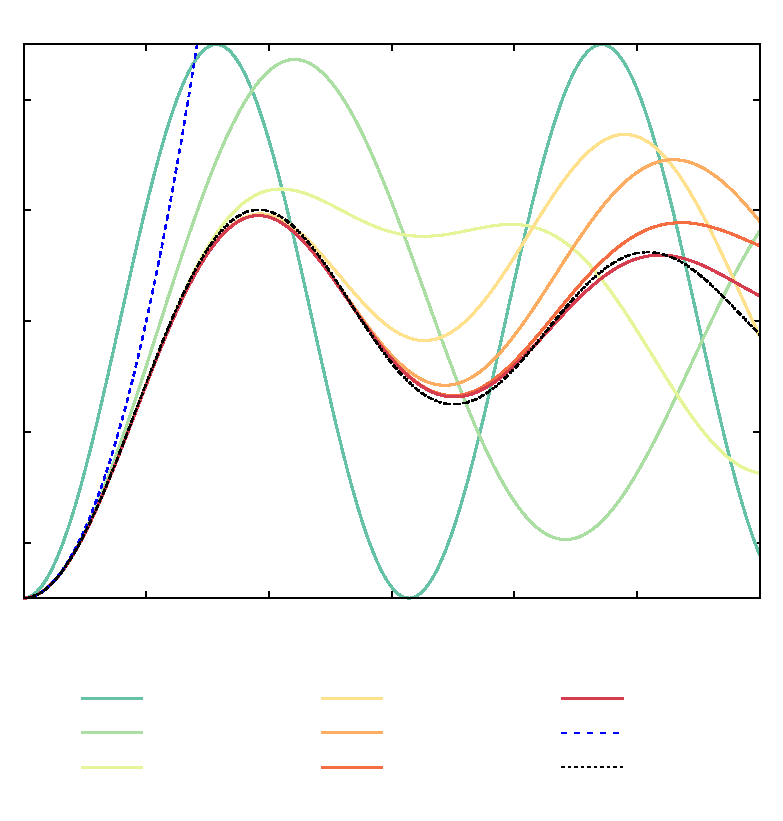
\includegraphics{kurzzeit}}%
    \gplfronttext
  \end{picture}%
\endgroup

    \caption{In color: Short-time evolution of the expectation value for the first spin of the total antiferromagnetic state \cref{eq:totalantif} for different $N$. In blue-dashed: Short-time approximation calculated by means of a Baker Campbell Hausdorff-expansion. In black-dashed: Theoretical calculation for an infinite-sized system.}
    \label{fig:kurzzeit}
\end{figure}

\subsection{Single magnon propagation}
The propagation of single or coupled spin flips in the form of ``magnons'' in a heisenberg chain is a current area of research. It is interesting to see, whether we can reproduce some of the qualitative findings of other publications. We begin by considering a single spin flip state in a length $N=31$ chain. The state is given by
\begin{align}
    \ket a =    \ket{\uparrow\uparrow\dots\uparrow\uparrow\downarrow\uparrow\uparrow\dots\uparrow\uparrow}.
    \label{eq:singlestate}
\end{align}
In \cref{fig:testsingle,fig:testsingle2,fig:testsingle3,fig:testsingle4,fig:testsingle5,fig:testsingle6,fig:testsingle7,fig:testsingle8,fig:testsingle9,fig:testsingle10,}, a spacetime matrix plot of the expactation value $\braket{S_i^z}_t$ is  plotted for $\mu=0$ and different values of NNN coupling $\lambda$. As one can see in \cref{fig:testsingle}, for $\lambda =0$ the single excitation magnon spreads with a well defined velocity of $J$, which is in agreement to recent studies on the topic, see \cite[p.\,101]{ganahl}. As confirmed by these studies, the propagation is in no way depending on the choice of $\mu$. The spin flip in the middle performs a damped oscillation, giving birth to multiple propagation cascades \cite[p.\,99]{ganahl}. The higher the NNN coupling, the more chaotic the propagation becomes. A particularly interesting feature is seen in \cref{fig:testsingle4}: A stable region with a close to zero expectation value forms in the middle. At even higher $\lambda$ it also propagates away but stays more or less bound. Note the differences at the boundary in comparison to \cite[p.\,101]{ganahl}, where no periodic boundary conditions were used. Also note that the time axis on the left has been properly scaled to make the different plots comparable. The higher $\lambda$, the faster the propagation occurs, which makes sense in the picture that the spin flips get ``pulled'' by more neighbors. The white peaks are a characteristic of finite systems and arise from magnons traveling in both directions hitting each other and interfering constructively. As this state is similar to the initial state, it corresponds to an echo peak in the Loschmidt echo. As the propagation velocity is $J$ (1 in our case), this peak occurs approximately at $t=J N$.
\begin{figure}[]
    \begin{subfigure}{.5\textwidth}
        \centering
        \resizebox{\textwidth}{!}{% GNUPLOT: LaTeX picture with Postscript
\begingroup
  \makeatletter
  \providecommand\color[2][]{%
    \GenericError{(gnuplot) \space\space\space\@spaces}{%
      Package color not loaded in conjunction with
      terminal option `colourtext'%
    }{See the gnuplot documentation for explanation.%
    }{Either use 'blacktext' in gnuplot or load the package
      color.sty in LaTeX.}%
    \renewcommand\color[2][]{}%
  }%
  \providecommand\includegraphics[2][]{%
    \GenericError{(gnuplot) \space\space\space\@spaces}{%
      Package graphicx or graphics not loaded%
    }{See the gnuplot documentation for explanation.%
    }{The gnuplot epslatex terminal needs graphicx.sty or graphics.sty.}%
    \renewcommand\includegraphics[2][]{}%
  }%
  \providecommand\rotatebox[2]{#2}%
  \@ifundefined{ifGPcolor}{%
    \newif\ifGPcolor
    \GPcolortrue
  }{}%
  \@ifundefined{ifGPblacktext}{%
    \newif\ifGPblacktext
    \GPblacktexttrue
  }{}%
  % define a \g@addto@macro without @ in the name:
  \let\gplgaddtomacro\g@addto@macro
  % define empty templates for all commands taking text:
  \gdef\gplbacktext{}%
  \gdef\gplfronttext{}%
  \makeatother
  \ifGPblacktext
    % no textcolor at all
    \def\colorrgb#1{}%
    \def\colorgray#1{}%
  \else
    % gray or color?
    \ifGPcolor
      \def\colorrgb#1{\color[rgb]{#1}}%
      \def\colorgray#1{\color[gray]{#1}}%
      \expandafter\def\csname LTw\endcsname{\color{white}}%
      \expandafter\def\csname LTb\endcsname{\color{black}}%
      \expandafter\def\csname LTa\endcsname{\color{black}}%
      \expandafter\def\csname LT0\endcsname{\color[rgb]{1,0,0}}%
      \expandafter\def\csname LT1\endcsname{\color[rgb]{0,1,0}}%
      \expandafter\def\csname LT2\endcsname{\color[rgb]{0,0,1}}%
      \expandafter\def\csname LT3\endcsname{\color[rgb]{1,0,1}}%
      \expandafter\def\csname LT4\endcsname{\color[rgb]{0,1,1}}%
      \expandafter\def\csname LT5\endcsname{\color[rgb]{1,1,0}}%
      \expandafter\def\csname LT6\endcsname{\color[rgb]{0,0,0}}%
      \expandafter\def\csname LT7\endcsname{\color[rgb]{1,0.3,0}}%
      \expandafter\def\csname LT8\endcsname{\color[rgb]{0.5,0.5,0.5}}%
    \else
      % gray
      \def\colorrgb#1{\color{black}}%
      \def\colorgray#1{\color[gray]{#1}}%
      \expandafter\def\csname LTw\endcsname{\color{white}}%
      \expandafter\def\csname LTb\endcsname{\color{black}}%
      \expandafter\def\csname LTa\endcsname{\color{black}}%
      \expandafter\def\csname LT0\endcsname{\color{black}}%
      \expandafter\def\csname LT1\endcsname{\color{black}}%
      \expandafter\def\csname LT2\endcsname{\color{black}}%
      \expandafter\def\csname LT3\endcsname{\color{black}}%
      \expandafter\def\csname LT4\endcsname{\color{black}}%
      \expandafter\def\csname LT5\endcsname{\color{black}}%
      \expandafter\def\csname LT6\endcsname{\color{black}}%
      \expandafter\def\csname LT7\endcsname{\color{black}}%
      \expandafter\def\csname LT8\endcsname{\color{black}}%
    \fi
  \fi
    \setlength{\unitlength}{0.0500bp}%
    \ifx\gptboxheight\undefined%
      \newlength{\gptboxheight}%
      \newlength{\gptboxwidth}%
      \newsavebox{\gptboxtext}%
    \fi%
    \setlength{\fboxrule}{0.5pt}%
    \setlength{\fboxsep}{1pt}%
\begin{picture}(5760.00,4320.00)%
    \gplgaddtomacro\gplbacktext{%
      \csname LTb\endcsname%
      \put(682,550){\makebox(0,0)[r]{\strut{}$0$}}%
      \put(682,1068){\makebox(0,0)[r]{\strut{}$10$}}%
      \put(682,1586){\makebox(0,0)[r]{\strut{}$20$}}%
      \put(682,2104){\makebox(0,0)[r]{\strut{}$30$}}%
      \put(682,2622){\makebox(0,0)[r]{\strut{}$40$}}%
      \put(682,3140){\makebox(0,0)[r]{\strut{}$50$}}%
      \put(682,3658){\makebox(0,0)[r]{\strut{}$60$}}%
      \put(873,330){\makebox(0,0){\strut{}$0$}}%
      \put(1468,330){\makebox(0,0){\strut{}$5$}}%
      \put(2062,330){\makebox(0,0){\strut{}$10$}}%
      \put(2656,330){\makebox(0,0){\strut{}$15$}}%
      \put(3250,330){\makebox(0,0){\strut{}$20$}}%
      \put(3844,330){\makebox(0,0){\strut{}$25$}}%
      \put(4439,330){\makebox(0,0){\strut{}$30$}}%
    }%
    \gplgaddtomacro\gplfronttext{%
      \csname LTb\endcsname%
      \put(176,2104){\rotatebox{-270}{\makebox(0,0){\strut{}time $Jt$}}}%
      \put(2656,0){\makebox(0,0){\strut{}particle index $i$}}%
      \put(2656,3989){\makebox(0,0){\strut{}$\mu=0,~\lambda=$0.0~$N=31$}}%
      \csname LTb\endcsname%
      \put(4906,550){\makebox(0,0)[l]{\strut{}$-0.5$}}%
      \put(4906,860){\makebox(0,0)[l]{\strut{}$-0.4$}}%
      \put(4906,1171){\makebox(0,0)[l]{\strut{}$-0.3$}}%
      \put(4906,1482){\makebox(0,0)[l]{\strut{}$-0.2$}}%
      \put(4906,1793){\makebox(0,0)[l]{\strut{}$-0.1$}}%
      \put(4906,2104){\makebox(0,0)[l]{\strut{}$0$}}%
      \put(4906,2415){\makebox(0,0)[l]{\strut{}$0.1$}}%
      \put(4906,2726){\makebox(0,0)[l]{\strut{}$0.2$}}%
      \put(4906,3037){\makebox(0,0)[l]{\strut{}$0.3$}}%
      \put(4906,3348){\makebox(0,0)[l]{\strut{}$0.4$}}%
      \put(4906,3659){\makebox(0,0)[l]{\strut{}$0.5$}}%
      \put(5500,2104){\rotatebox{-270}{\makebox(0,0){\strut{}$\braket{S_1^z}_t$}}}%
    }%
    \gplbacktext
    \put(0,0){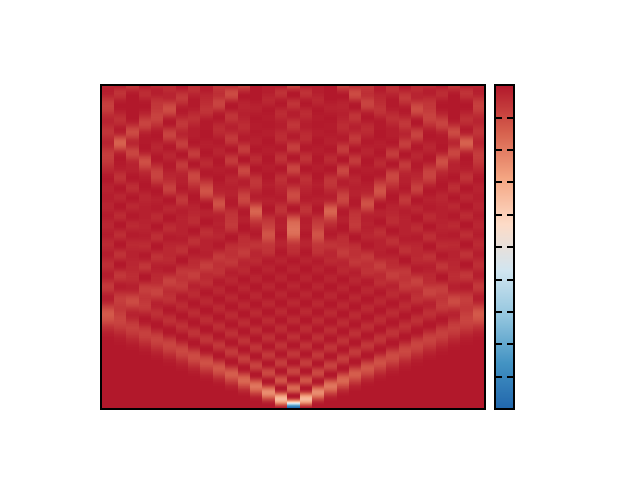
\includegraphics{Sz_l0_0}}%
    \gplfronttext
  \end{picture}%
\endgroup
}
        \caption{$\lambda=0$}
        \label{fig:testsingle}
    \end{subfigure}
    \begin{subfigure}{.5\textwidth}
        \centering
        \resizebox{\textwidth}{!}{% GNUPLOT: LaTeX picture with Postscript
\begingroup
  \makeatletter
  \providecommand\color[2][]{%
    \GenericError{(gnuplot) \space\space\space\@spaces}{%
      Package color not loaded in conjunction with
      terminal option `colourtext'%
    }{See the gnuplot documentation for explanation.%
    }{Either use 'blacktext' in gnuplot or load the package
      color.sty in LaTeX.}%
    \renewcommand\color[2][]{}%
  }%
  \providecommand\includegraphics[2][]{%
    \GenericError{(gnuplot) \space\space\space\@spaces}{%
      Package graphicx or graphics not loaded%
    }{See the gnuplot documentation for explanation.%
    }{The gnuplot epslatex terminal needs graphicx.sty or graphics.sty.}%
    \renewcommand\includegraphics[2][]{}%
  }%
  \providecommand\rotatebox[2]{#2}%
  \@ifundefined{ifGPcolor}{%
    \newif\ifGPcolor
    \GPcolortrue
  }{}%
  \@ifundefined{ifGPblacktext}{%
    \newif\ifGPblacktext
    \GPblacktexttrue
  }{}%
  % define a \g@addto@macro without @ in the name:
  \let\gplgaddtomacro\g@addto@macro
  % define empty templates for all commands taking text:
  \gdef\gplbacktext{}%
  \gdef\gplfronttext{}%
  \makeatother
  \ifGPblacktext
    % no textcolor at all
    \def\colorrgb#1{}%
    \def\colorgray#1{}%
  \else
    % gray or color?
    \ifGPcolor
      \def\colorrgb#1{\color[rgb]{#1}}%
      \def\colorgray#1{\color[gray]{#1}}%
      \expandafter\def\csname LTw\endcsname{\color{white}}%
      \expandafter\def\csname LTb\endcsname{\color{black}}%
      \expandafter\def\csname LTa\endcsname{\color{black}}%
      \expandafter\def\csname LT0\endcsname{\color[rgb]{1,0,0}}%
      \expandafter\def\csname LT1\endcsname{\color[rgb]{0,1,0}}%
      \expandafter\def\csname LT2\endcsname{\color[rgb]{0,0,1}}%
      \expandafter\def\csname LT3\endcsname{\color[rgb]{1,0,1}}%
      \expandafter\def\csname LT4\endcsname{\color[rgb]{0,1,1}}%
      \expandafter\def\csname LT5\endcsname{\color[rgb]{1,1,0}}%
      \expandafter\def\csname LT6\endcsname{\color[rgb]{0,0,0}}%
      \expandafter\def\csname LT7\endcsname{\color[rgb]{1,0.3,0}}%
      \expandafter\def\csname LT8\endcsname{\color[rgb]{0.5,0.5,0.5}}%
    \else
      % gray
      \def\colorrgb#1{\color{black}}%
      \def\colorgray#1{\color[gray]{#1}}%
      \expandafter\def\csname LTw\endcsname{\color{white}}%
      \expandafter\def\csname LTb\endcsname{\color{black}}%
      \expandafter\def\csname LTa\endcsname{\color{black}}%
      \expandafter\def\csname LT0\endcsname{\color{black}}%
      \expandafter\def\csname LT1\endcsname{\color{black}}%
      \expandafter\def\csname LT2\endcsname{\color{black}}%
      \expandafter\def\csname LT3\endcsname{\color{black}}%
      \expandafter\def\csname LT4\endcsname{\color{black}}%
      \expandafter\def\csname LT5\endcsname{\color{black}}%
      \expandafter\def\csname LT6\endcsname{\color{black}}%
      \expandafter\def\csname LT7\endcsname{\color{black}}%
      \expandafter\def\csname LT8\endcsname{\color{black}}%
    \fi
  \fi
    \setlength{\unitlength}{0.0500bp}%
    \ifx\gptboxheight\undefined%
      \newlength{\gptboxheight}%
      \newlength{\gptboxwidth}%
      \newsavebox{\gptboxtext}%
    \fi%
    \setlength{\fboxrule}{0.5pt}%
    \setlength{\fboxsep}{1pt}%
\begin{picture}(5760.00,4320.00)%
    \gplgaddtomacro\gplbacktext{%
      \csname LTb\endcsname%
      \put(682,550){\makebox(0,0)[r]{\strut{}$0$}}%
      \put(682,1115){\makebox(0,0)[r]{\strut{}$10$}}%
      \put(682,1680){\makebox(0,0)[r]{\strut{}$20$}}%
      \put(682,2245){\makebox(0,0)[r]{\strut{}$30$}}%
      \put(682,2811){\makebox(0,0)[r]{\strut{}$40$}}%
      \put(682,3376){\makebox(0,0)[r]{\strut{}$50$}}%
      \put(873,330){\makebox(0,0){\strut{}$0$}}%
      \put(1468,330){\makebox(0,0){\strut{}$5$}}%
      \put(2062,330){\makebox(0,0){\strut{}$10$}}%
      \put(2656,330){\makebox(0,0){\strut{}$15$}}%
      \put(3250,330){\makebox(0,0){\strut{}$20$}}%
      \put(3844,330){\makebox(0,0){\strut{}$25$}}%
      \put(4439,330){\makebox(0,0){\strut{}$30$}}%
    }%
    \gplgaddtomacro\gplfronttext{%
      \csname LTb\endcsname%
      \put(176,2104){\rotatebox{-270}{\makebox(0,0){\strut{}time $Jt$}}}%
      \put(2656,0){\makebox(0,0){\strut{}particle index $i$}}%
      \put(2656,3989){\makebox(0,0){\strut{}$\mu=0,~\lambda=$0.1~$N=31$}}%
      \csname LTb\endcsname%
      \put(4906,550){\makebox(0,0)[l]{\strut{}$-0.5$}}%
      \put(4906,860){\makebox(0,0)[l]{\strut{}$-0.4$}}%
      \put(4906,1171){\makebox(0,0)[l]{\strut{}$-0.3$}}%
      \put(4906,1482){\makebox(0,0)[l]{\strut{}$-0.2$}}%
      \put(4906,1793){\makebox(0,0)[l]{\strut{}$-0.1$}}%
      \put(4906,2104){\makebox(0,0)[l]{\strut{}$0$}}%
      \put(4906,2415){\makebox(0,0)[l]{\strut{}$0.1$}}%
      \put(4906,2726){\makebox(0,0)[l]{\strut{}$0.2$}}%
      \put(4906,3037){\makebox(0,0)[l]{\strut{}$0.3$}}%
      \put(4906,3348){\makebox(0,0)[l]{\strut{}$0.4$}}%
      \put(4906,3659){\makebox(0,0)[l]{\strut{}$0.5$}}%
      \put(5500,2104){\rotatebox{-270}{\makebox(0,0){\strut{}$\braket{S_1^z}_t$}}}%
    }%
    \gplbacktext
    \put(0,0){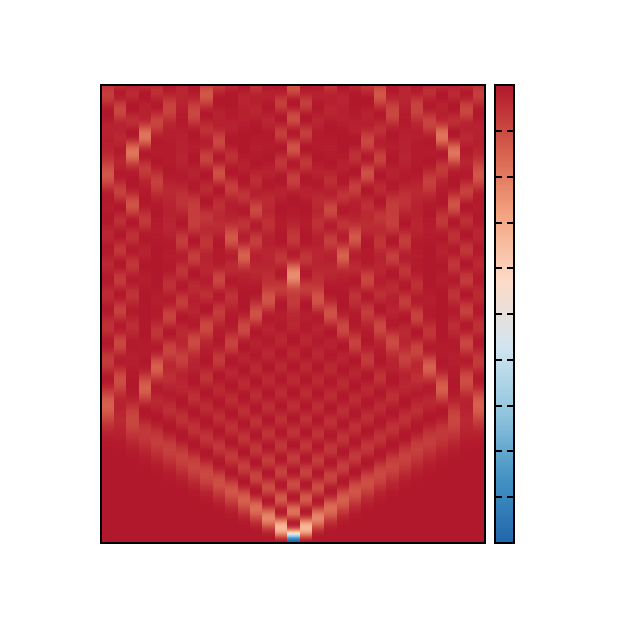
\includegraphics{Sz_l0_1}}%
    \gplfronttext
  \end{picture}%
\endgroup
}
        \caption{$\lambda=0.1$}
        \label{fig:testsingle2}
    \end{subfigure} 
    \begin{subfigure}{.5\textwidth}
        \centering
        \resizebox{\textwidth}{!}{% GNUPLOT: LaTeX picture with Postscript
\begingroup
  \makeatletter
  \providecommand\color[2][]{%
    \GenericError{(gnuplot) \space\space\space\@spaces}{%
      Package color not loaded in conjunction with
      terminal option `colourtext'%
    }{See the gnuplot documentation for explanation.%
    }{Either use 'blacktext' in gnuplot or load the package
      color.sty in LaTeX.}%
    \renewcommand\color[2][]{}%
  }%
  \providecommand\includegraphics[2][]{%
    \GenericError{(gnuplot) \space\space\space\@spaces}{%
      Package graphicx or graphics not loaded%
    }{See the gnuplot documentation for explanation.%
    }{The gnuplot epslatex terminal needs graphicx.sty or graphics.sty.}%
    \renewcommand\includegraphics[2][]{}%
  }%
  \providecommand\rotatebox[2]{#2}%
  \@ifundefined{ifGPcolor}{%
    \newif\ifGPcolor
    \GPcolortrue
  }{}%
  \@ifundefined{ifGPblacktext}{%
    \newif\ifGPblacktext
    \GPblacktexttrue
  }{}%
  % define a \g@addto@macro without @ in the name:
  \let\gplgaddtomacro\g@addto@macro
  % define empty templates for all commands taking text:
  \gdef\gplbacktext{}%
  \gdef\gplfronttext{}%
  \makeatother
  \ifGPblacktext
    % no textcolor at all
    \def\colorrgb#1{}%
    \def\colorgray#1{}%
  \else
    % gray or color?
    \ifGPcolor
      \def\colorrgb#1{\color[rgb]{#1}}%
      \def\colorgray#1{\color[gray]{#1}}%
      \expandafter\def\csname LTw\endcsname{\color{white}}%
      \expandafter\def\csname LTb\endcsname{\color{black}}%
      \expandafter\def\csname LTa\endcsname{\color{black}}%
      \expandafter\def\csname LT0\endcsname{\color[rgb]{1,0,0}}%
      \expandafter\def\csname LT1\endcsname{\color[rgb]{0,1,0}}%
      \expandafter\def\csname LT2\endcsname{\color[rgb]{0,0,1}}%
      \expandafter\def\csname LT3\endcsname{\color[rgb]{1,0,1}}%
      \expandafter\def\csname LT4\endcsname{\color[rgb]{0,1,1}}%
      \expandafter\def\csname LT5\endcsname{\color[rgb]{1,1,0}}%
      \expandafter\def\csname LT6\endcsname{\color[rgb]{0,0,0}}%
      \expandafter\def\csname LT7\endcsname{\color[rgb]{1,0.3,0}}%
      \expandafter\def\csname LT8\endcsname{\color[rgb]{0.5,0.5,0.5}}%
    \else
      % gray
      \def\colorrgb#1{\color{black}}%
      \def\colorgray#1{\color[gray]{#1}}%
      \expandafter\def\csname LTw\endcsname{\color{white}}%
      \expandafter\def\csname LTb\endcsname{\color{black}}%
      \expandafter\def\csname LTa\endcsname{\color{black}}%
      \expandafter\def\csname LT0\endcsname{\color{black}}%
      \expandafter\def\csname LT1\endcsname{\color{black}}%
      \expandafter\def\csname LT2\endcsname{\color{black}}%
      \expandafter\def\csname LT3\endcsname{\color{black}}%
      \expandafter\def\csname LT4\endcsname{\color{black}}%
      \expandafter\def\csname LT5\endcsname{\color{black}}%
      \expandafter\def\csname LT6\endcsname{\color{black}}%
      \expandafter\def\csname LT7\endcsname{\color{black}}%
      \expandafter\def\csname LT8\endcsname{\color{black}}%
    \fi
  \fi
    \setlength{\unitlength}{0.0500bp}%
    \ifx\gptboxheight\undefined%
      \newlength{\gptboxheight}%
      \newlength{\gptboxwidth}%
      \newsavebox{\gptboxtext}%
    \fi%
    \setlength{\fboxrule}{0.5pt}%
    \setlength{\fboxsep}{1pt}%
\begin{picture}(5760.00,4320.00)%
    \gplgaddtomacro\gplbacktext{%
      \csname LTb\endcsname%
      \put(682,550){\makebox(0,0)[r]{\strut{}$0$}}%
      \put(682,1172){\makebox(0,0)[r]{\strut{}$10$}}%
      \put(682,1793){\makebox(0,0)[r]{\strut{}$20$}}%
      \put(682,2415){\makebox(0,0)[r]{\strut{}$30$}}%
      \put(682,3037){\makebox(0,0)[r]{\strut{}$40$}}%
      \put(682,3658){\makebox(0,0)[r]{\strut{}$50$}}%
      \put(873,330){\makebox(0,0){\strut{}$0$}}%
      \put(1468,330){\makebox(0,0){\strut{}$5$}}%
      \put(2062,330){\makebox(0,0){\strut{}$10$}}%
      \put(2656,330){\makebox(0,0){\strut{}$15$}}%
      \put(3250,330){\makebox(0,0){\strut{}$20$}}%
      \put(3844,330){\makebox(0,0){\strut{}$25$}}%
      \put(4439,330){\makebox(0,0){\strut{}$30$}}%
    }%
    \gplgaddtomacro\gplfronttext{%
      \csname LTb\endcsname%
      \put(176,2104){\rotatebox{-270}{\makebox(0,0){\strut{}time $Jt$}}}%
      \put(2656,0){\makebox(0,0){\strut{}particle index $i$}}%
      \put(2656,3989){\makebox(0,0){\strut{}$\mu=0,~\lambda=$0.2~$N=31$}}%
      \csname LTb\endcsname%
      \put(4906,550){\makebox(0,0)[l]{\strut{}$-0.5$}}%
      \put(4906,860){\makebox(0,0)[l]{\strut{}$-0.4$}}%
      \put(4906,1171){\makebox(0,0)[l]{\strut{}$-0.3$}}%
      \put(4906,1482){\makebox(0,0)[l]{\strut{}$-0.2$}}%
      \put(4906,1793){\makebox(0,0)[l]{\strut{}$-0.1$}}%
      \put(4906,2104){\makebox(0,0)[l]{\strut{}$0$}}%
      \put(4906,2415){\makebox(0,0)[l]{\strut{}$0.1$}}%
      \put(4906,2726){\makebox(0,0)[l]{\strut{}$0.2$}}%
      \put(4906,3037){\makebox(0,0)[l]{\strut{}$0.3$}}%
      \put(4906,3348){\makebox(0,0)[l]{\strut{}$0.4$}}%
      \put(4906,3659){\makebox(0,0)[l]{\strut{}$0.5$}}%
      \put(5500,2104){\rotatebox{-270}{\makebox(0,0){\strut{}$\braket{S_1^z}_t$}}}%
    }%
    \gplbacktext
    \put(0,0){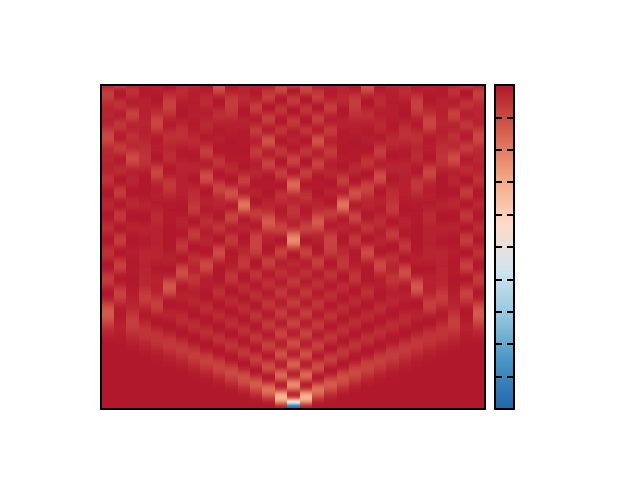
\includegraphics{Sz_l0_2}}%
    \gplfronttext
  \end{picture}%
\endgroup
}
        \caption{$\lambda=0.2$}
        \label{fig:testsingle3}
    \end{subfigure}
    \begin{subfigure}{.5\textwidth}
        \centering
        \resizebox{\textwidth}{!}{% GNUPLOT: LaTeX picture with Postscript
\begingroup
  \makeatletter
  \providecommand\color[2][]{%
    \GenericError{(gnuplot) \space\space\space\@spaces}{%
      Package color not loaded in conjunction with
      terminal option `colourtext'%
    }{See the gnuplot documentation for explanation.%
    }{Either use 'blacktext' in gnuplot or load the package
      color.sty in LaTeX.}%
    \renewcommand\color[2][]{}%
  }%
  \providecommand\includegraphics[2][]{%
    \GenericError{(gnuplot) \space\space\space\@spaces}{%
      Package graphicx or graphics not loaded%
    }{See the gnuplot documentation for explanation.%
    }{The gnuplot epslatex terminal needs graphicx.sty or graphics.sty.}%
    \renewcommand\includegraphics[2][]{}%
  }%
  \providecommand\rotatebox[2]{#2}%
  \@ifundefined{ifGPcolor}{%
    \newif\ifGPcolor
    \GPcolortrue
  }{}%
  \@ifundefined{ifGPblacktext}{%
    \newif\ifGPblacktext
    \GPblacktexttrue
  }{}%
  % define a \g@addto@macro without @ in the name:
  \let\gplgaddtomacro\g@addto@macro
  % define empty templates for all commands taking text:
  \gdef\gplbacktext{}%
  \gdef\gplfronttext{}%
  \makeatother
  \ifGPblacktext
    % no textcolor at all
    \def\colorrgb#1{}%
    \def\colorgray#1{}%
  \else
    % gray or color?
    \ifGPcolor
      \def\colorrgb#1{\color[rgb]{#1}}%
      \def\colorgray#1{\color[gray]{#1}}%
      \expandafter\def\csname LTw\endcsname{\color{white}}%
      \expandafter\def\csname LTb\endcsname{\color{black}}%
      \expandafter\def\csname LTa\endcsname{\color{black}}%
      \expandafter\def\csname LT0\endcsname{\color[rgb]{1,0,0}}%
      \expandafter\def\csname LT1\endcsname{\color[rgb]{0,1,0}}%
      \expandafter\def\csname LT2\endcsname{\color[rgb]{0,0,1}}%
      \expandafter\def\csname LT3\endcsname{\color[rgb]{1,0,1}}%
      \expandafter\def\csname LT4\endcsname{\color[rgb]{0,1,1}}%
      \expandafter\def\csname LT5\endcsname{\color[rgb]{1,1,0}}%
      \expandafter\def\csname LT6\endcsname{\color[rgb]{0,0,0}}%
      \expandafter\def\csname LT7\endcsname{\color[rgb]{1,0.3,0}}%
      \expandafter\def\csname LT8\endcsname{\color[rgb]{0.5,0.5,0.5}}%
    \else
      % gray
      \def\colorrgb#1{\color{black}}%
      \def\colorgray#1{\color[gray]{#1}}%
      \expandafter\def\csname LTw\endcsname{\color{white}}%
      \expandafter\def\csname LTb\endcsname{\color{black}}%
      \expandafter\def\csname LTa\endcsname{\color{black}}%
      \expandafter\def\csname LT0\endcsname{\color{black}}%
      \expandafter\def\csname LT1\endcsname{\color{black}}%
      \expandafter\def\csname LT2\endcsname{\color{black}}%
      \expandafter\def\csname LT3\endcsname{\color{black}}%
      \expandafter\def\csname LT4\endcsname{\color{black}}%
      \expandafter\def\csname LT5\endcsname{\color{black}}%
      \expandafter\def\csname LT6\endcsname{\color{black}}%
      \expandafter\def\csname LT7\endcsname{\color{black}}%
      \expandafter\def\csname LT8\endcsname{\color{black}}%
    \fi
  \fi
    \setlength{\unitlength}{0.0500bp}%
    \ifx\gptboxheight\undefined%
      \newlength{\gptboxheight}%
      \newlength{\gptboxwidth}%
      \newsavebox{\gptboxtext}%
    \fi%
    \setlength{\fboxrule}{0.5pt}%
    \setlength{\fboxsep}{1pt}%
\begin{picture}(5760.00,5760.00)%
    \gplgaddtomacro\gplbacktext{%
      \csname LTb\endcsname%
      \put(682,704){\makebox(0,0)[r]{\strut{}$0$}}%
      \put(682,1193){\makebox(0,0)[r]{\strut{}$5$}}%
      \put(682,1681){\makebox(0,0)[r]{\strut{}$10$}}%
      \put(682,2169){\makebox(0,0)[r]{\strut{}$15$}}%
      \put(682,2657){\makebox(0,0)[r]{\strut{}$20$}}%
      \put(682,3145){\makebox(0,0)[r]{\strut{}$25$}}%
      \put(682,3633){\makebox(0,0)[r]{\strut{}$30$}}%
      \put(682,4121){\makebox(0,0)[r]{\strut{}$35$}}%
      \put(682,4609){\makebox(0,0)[r]{\strut{}$40$}}%
      \put(682,5098){\makebox(0,0)[r]{\strut{}$45$}}%
      \put(873,484){\makebox(0,0){\strut{}$0$}}%
      \put(1468,484){\makebox(0,0){\strut{}$5$}}%
      \put(2062,484){\makebox(0,0){\strut{}$10$}}%
      \put(2656,484){\makebox(0,0){\strut{}$15$}}%
      \put(3250,484){\makebox(0,0){\strut{}$20$}}%
      \put(3844,484){\makebox(0,0){\strut{}$25$}}%
      \put(4439,484){\makebox(0,0){\strut{}$30$}}%
    }%
    \gplgaddtomacro\gplfronttext{%
      \csname LTb\endcsname%
      \put(176,2901){\rotatebox{-270}{\makebox(0,0){\strut{}time $t$}}}%
      \put(2656,154){\makebox(0,0){\strut{}particle index $i$}}%
      \put(2656,5429){\makebox(0,0){\strut{}$\mu=0,~\lambda=$0.3}}%
      \csname LTb\endcsname%
      \put(4906,704){\makebox(0,0)[l]{\strut{}$-0.5$}}%
      \put(4906,1143){\makebox(0,0)[l]{\strut{}$-0.4$}}%
      \put(4906,1583){\makebox(0,0)[l]{\strut{}$-0.3$}}%
      \put(4906,2022){\makebox(0,0)[l]{\strut{}$-0.2$}}%
      \put(4906,2462){\makebox(0,0)[l]{\strut{}$-0.1$}}%
      \put(4906,2901){\makebox(0,0)[l]{\strut{}$0$}}%
      \put(4906,3341){\makebox(0,0)[l]{\strut{}$0.1$}}%
      \put(4906,3780){\makebox(0,0)[l]{\strut{}$0.2$}}%
      \put(4906,4220){\makebox(0,0)[l]{\strut{}$0.3$}}%
      \put(4906,4659){\makebox(0,0)[l]{\strut{}$0.4$}}%
      \put(4906,5099){\makebox(0,0)[l]{\strut{}$0.5$}}%
      \put(5500,2901){\rotatebox{-270}{\makebox(0,0){\strut{}$\braket{S_1^z}_t$}}}%
    }%
    \gplbacktext
    \put(0,0){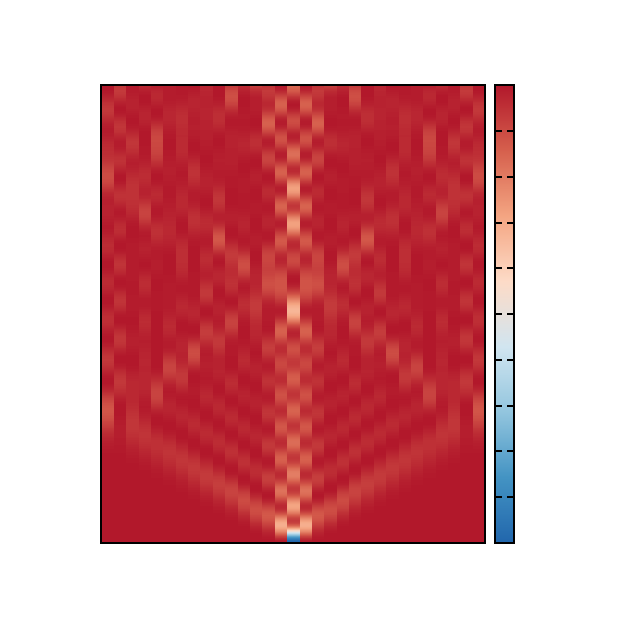
\includegraphics{Sz_l0_3}}%
    \gplfronttext
  \end{picture}%
\endgroup
}
        \caption{$\lambda=0.3$}
        \label{fig:testsingle4}
    \end{subfigure}
    \begin{subfigure}{.5\textwidth}
        \centering
        \resizebox{\textwidth}{!}{% GNUPLOT: LaTeX picture with Postscript
\begingroup
  \makeatletter
  \providecommand\color[2][]{%
    \GenericError{(gnuplot) \space\space\space\@spaces}{%
      Package color not loaded in conjunction with
      terminal option `colourtext'%
    }{See the gnuplot documentation for explanation.%
    }{Either use 'blacktext' in gnuplot or load the package
      color.sty in LaTeX.}%
    \renewcommand\color[2][]{}%
  }%
  \providecommand\includegraphics[2][]{%
    \GenericError{(gnuplot) \space\space\space\@spaces}{%
      Package graphicx or graphics not loaded%
    }{See the gnuplot documentation for explanation.%
    }{The gnuplot epslatex terminal needs graphicx.sty or graphics.sty.}%
    \renewcommand\includegraphics[2][]{}%
  }%
  \providecommand\rotatebox[2]{#2}%
  \@ifundefined{ifGPcolor}{%
    \newif\ifGPcolor
    \GPcolortrue
  }{}%
  \@ifundefined{ifGPblacktext}{%
    \newif\ifGPblacktext
    \GPblacktexttrue
  }{}%
  % define a \g@addto@macro without @ in the name:
  \let\gplgaddtomacro\g@addto@macro
  % define empty templates for all commands taking text:
  \gdef\gplbacktext{}%
  \gdef\gplfronttext{}%
  \makeatother
  \ifGPblacktext
    % no textcolor at all
    \def\colorrgb#1{}%
    \def\colorgray#1{}%
  \else
    % gray or color?
    \ifGPcolor
      \def\colorrgb#1{\color[rgb]{#1}}%
      \def\colorgray#1{\color[gray]{#1}}%
      \expandafter\def\csname LTw\endcsname{\color{white}}%
      \expandafter\def\csname LTb\endcsname{\color{black}}%
      \expandafter\def\csname LTa\endcsname{\color{black}}%
      \expandafter\def\csname LT0\endcsname{\color[rgb]{1,0,0}}%
      \expandafter\def\csname LT1\endcsname{\color[rgb]{0,1,0}}%
      \expandafter\def\csname LT2\endcsname{\color[rgb]{0,0,1}}%
      \expandafter\def\csname LT3\endcsname{\color[rgb]{1,0,1}}%
      \expandafter\def\csname LT4\endcsname{\color[rgb]{0,1,1}}%
      \expandafter\def\csname LT5\endcsname{\color[rgb]{1,1,0}}%
      \expandafter\def\csname LT6\endcsname{\color[rgb]{0,0,0}}%
      \expandafter\def\csname LT7\endcsname{\color[rgb]{1,0.3,0}}%
      \expandafter\def\csname LT8\endcsname{\color[rgb]{0.5,0.5,0.5}}%
    \else
      % gray
      \def\colorrgb#1{\color{black}}%
      \def\colorgray#1{\color[gray]{#1}}%
      \expandafter\def\csname LTw\endcsname{\color{white}}%
      \expandafter\def\csname LTb\endcsname{\color{black}}%
      \expandafter\def\csname LTa\endcsname{\color{black}}%
      \expandafter\def\csname LT0\endcsname{\color{black}}%
      \expandafter\def\csname LT1\endcsname{\color{black}}%
      \expandafter\def\csname LT2\endcsname{\color{black}}%
      \expandafter\def\csname LT3\endcsname{\color{black}}%
      \expandafter\def\csname LT4\endcsname{\color{black}}%
      \expandafter\def\csname LT5\endcsname{\color{black}}%
      \expandafter\def\csname LT6\endcsname{\color{black}}%
      \expandafter\def\csname LT7\endcsname{\color{black}}%
      \expandafter\def\csname LT8\endcsname{\color{black}}%
    \fi
  \fi
    \setlength{\unitlength}{0.0500bp}%
    \ifx\gptboxheight\undefined%
      \newlength{\gptboxheight}%
      \newlength{\gptboxwidth}%
      \newsavebox{\gptboxtext}%
    \fi%
    \setlength{\fboxrule}{0.5pt}%
    \setlength{\fboxsep}{1pt}%
\begin{picture}(5760.00,5760.00)%
    \gplgaddtomacro\gplbacktext{%
      \csname LTb\endcsname%
      \put(682,705){\makebox(0,0)[r]{\strut{}$0$}}%
      \put(682,1254){\makebox(0,0)[r]{\strut{}$5$}}%
      \put(682,1803){\makebox(0,0)[r]{\strut{}$10$}}%
      \put(682,2352){\makebox(0,0)[r]{\strut{}$15$}}%
      \put(682,2901){\makebox(0,0)[r]{\strut{}$20$}}%
      \put(682,3451){\makebox(0,0)[r]{\strut{}$25$}}%
      \put(682,4000){\makebox(0,0)[r]{\strut{}$30$}}%
      \put(682,4549){\makebox(0,0)[r]{\strut{}$35$}}%
      \put(682,5098){\makebox(0,0)[r]{\strut{}$40$}}%
      \put(873,484){\makebox(0,0){\strut{}$0$}}%
      \put(1468,484){\makebox(0,0){\strut{}$5$}}%
      \put(2062,484){\makebox(0,0){\strut{}$10$}}%
      \put(2656,484){\makebox(0,0){\strut{}$15$}}%
      \put(3250,484){\makebox(0,0){\strut{}$20$}}%
      \put(3844,484){\makebox(0,0){\strut{}$25$}}%
      \put(4439,484){\makebox(0,0){\strut{}$30$}}%
    }%
    \gplgaddtomacro\gplfronttext{%
      \csname LTb\endcsname%
      \put(176,2901){\rotatebox{-270}{\makebox(0,0){\strut{}time $t$}}}%
      \put(2656,154){\makebox(0,0){\strut{}particle index $i$}}%
      \put(2656,5429){\makebox(0,0){\strut{}$\mu=0,~\lambda=$0.4}}%
      \csname LTb\endcsname%
      \put(4906,704){\makebox(0,0)[l]{\strut{}$-0.5$}}%
      \put(4906,1143){\makebox(0,0)[l]{\strut{}$-0.4$}}%
      \put(4906,1583){\makebox(0,0)[l]{\strut{}$-0.3$}}%
      \put(4906,2022){\makebox(0,0)[l]{\strut{}$-0.2$}}%
      \put(4906,2462){\makebox(0,0)[l]{\strut{}$-0.1$}}%
      \put(4906,2901){\makebox(0,0)[l]{\strut{}$0$}}%
      \put(4906,3341){\makebox(0,0)[l]{\strut{}$0.1$}}%
      \put(4906,3780){\makebox(0,0)[l]{\strut{}$0.2$}}%
      \put(4906,4220){\makebox(0,0)[l]{\strut{}$0.3$}}%
      \put(4906,4659){\makebox(0,0)[l]{\strut{}$0.4$}}%
      \put(4906,5099){\makebox(0,0)[l]{\strut{}$0.5$}}%
      \put(5500,2901){\rotatebox{-270}{\makebox(0,0){\strut{}$\braket{S_1^z}_t$}}}%
    }%
    \gplbacktext
    \put(0,0){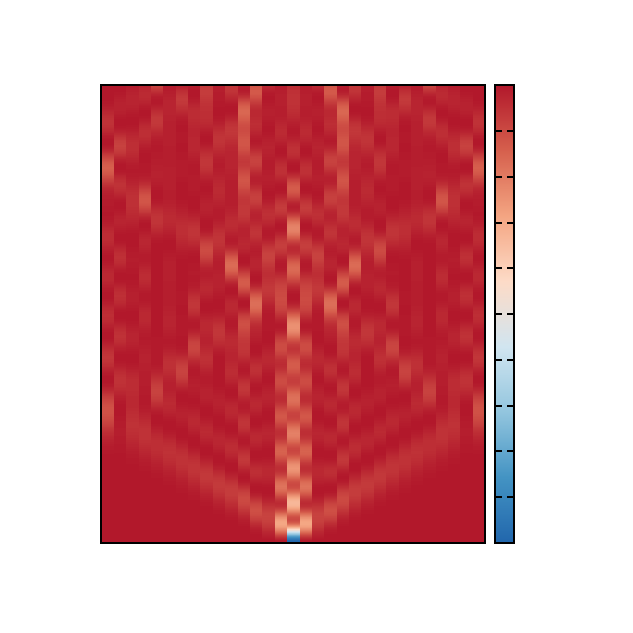
\includegraphics{Sz_l0_4}}%
    \gplfronttext
  \end{picture}%
\endgroup
}
        \caption{$\lambda=0.4$}
        \label{fig:testsingle5}
    \end{subfigure}
    \begin{subfigure}{.5\textwidth}
        \centering
        \resizebox{\textwidth}{!}{% GNUPLOT: LaTeX picture with Postscript
\begingroup
  \makeatletter
  \providecommand\color[2][]{%
    \GenericError{(gnuplot) \space\space\space\@spaces}{%
      Package color not loaded in conjunction with
      terminal option `colourtext'%
    }{See the gnuplot documentation for explanation.%
    }{Either use 'blacktext' in gnuplot or load the package
      color.sty in LaTeX.}%
    \renewcommand\color[2][]{}%
  }%
  \providecommand\includegraphics[2][]{%
    \GenericError{(gnuplot) \space\space\space\@spaces}{%
      Package graphicx or graphics not loaded%
    }{See the gnuplot documentation for explanation.%
    }{The gnuplot epslatex terminal needs graphicx.sty or graphics.sty.}%
    \renewcommand\includegraphics[2][]{}%
  }%
  \providecommand\rotatebox[2]{#2}%
  \@ifundefined{ifGPcolor}{%
    \newif\ifGPcolor
    \GPcolortrue
  }{}%
  \@ifundefined{ifGPblacktext}{%
    \newif\ifGPblacktext
    \GPblacktexttrue
  }{}%
  % define a \g@addto@macro without @ in the name:
  \let\gplgaddtomacro\g@addto@macro
  % define empty templates for all commands taking text:
  \gdef\gplbacktext{}%
  \gdef\gplfronttext{}%
  \makeatother
  \ifGPblacktext
    % no textcolor at all
    \def\colorrgb#1{}%
    \def\colorgray#1{}%
  \else
    % gray or color?
    \ifGPcolor
      \def\colorrgb#1{\color[rgb]{#1}}%
      \def\colorgray#1{\color[gray]{#1}}%
      \expandafter\def\csname LTw\endcsname{\color{white}}%
      \expandafter\def\csname LTb\endcsname{\color{black}}%
      \expandafter\def\csname LTa\endcsname{\color{black}}%
      \expandafter\def\csname LT0\endcsname{\color[rgb]{1,0,0}}%
      \expandafter\def\csname LT1\endcsname{\color[rgb]{0,1,0}}%
      \expandafter\def\csname LT2\endcsname{\color[rgb]{0,0,1}}%
      \expandafter\def\csname LT3\endcsname{\color[rgb]{1,0,1}}%
      \expandafter\def\csname LT4\endcsname{\color[rgb]{0,1,1}}%
      \expandafter\def\csname LT5\endcsname{\color[rgb]{1,1,0}}%
      \expandafter\def\csname LT6\endcsname{\color[rgb]{0,0,0}}%
      \expandafter\def\csname LT7\endcsname{\color[rgb]{1,0.3,0}}%
      \expandafter\def\csname LT8\endcsname{\color[rgb]{0.5,0.5,0.5}}%
    \else
      % gray
      \def\colorrgb#1{\color{black}}%
      \def\colorgray#1{\color[gray]{#1}}%
      \expandafter\def\csname LTw\endcsname{\color{white}}%
      \expandafter\def\csname LTb\endcsname{\color{black}}%
      \expandafter\def\csname LTa\endcsname{\color{black}}%
      \expandafter\def\csname LT0\endcsname{\color{black}}%
      \expandafter\def\csname LT1\endcsname{\color{black}}%
      \expandafter\def\csname LT2\endcsname{\color{black}}%
      \expandafter\def\csname LT3\endcsname{\color{black}}%
      \expandafter\def\csname LT4\endcsname{\color{black}}%
      \expandafter\def\csname LT5\endcsname{\color{black}}%
      \expandafter\def\csname LT6\endcsname{\color{black}}%
      \expandafter\def\csname LT7\endcsname{\color{black}}%
      \expandafter\def\csname LT8\endcsname{\color{black}}%
    \fi
  \fi
    \setlength{\unitlength}{0.0500bp}%
    \ifx\gptboxheight\undefined%
      \newlength{\gptboxheight}%
      \newlength{\gptboxwidth}%
      \newsavebox{\gptboxtext}%
    \fi%
    \setlength{\fboxrule}{0.5pt}%
    \setlength{\fboxsep}{1pt}%
\begin{picture}(5760.00,5760.00)%
    \gplgaddtomacro\gplbacktext{%
      \csname LTb\endcsname%
      \put(682,705){\makebox(0,0)[r]{\strut{}$0$}}%
      \put(682,1332){\makebox(0,0)[r]{\strut{}$5$}}%
      \put(682,1960){\makebox(0,0)[r]{\strut{}$10$}}%
      \put(682,2588){\makebox(0,0)[r]{\strut{}$15$}}%
      \put(682,3215){\makebox(0,0)[r]{\strut{}$20$}}%
      \put(682,3843){\makebox(0,0)[r]{\strut{}$25$}}%
      \put(682,4471){\makebox(0,0)[r]{\strut{}$30$}}%
      \put(682,5098){\makebox(0,0)[r]{\strut{}$35$}}%
      \put(873,484){\makebox(0,0){\strut{}$0$}}%
      \put(1468,484){\makebox(0,0){\strut{}$5$}}%
      \put(2062,484){\makebox(0,0){\strut{}$10$}}%
      \put(2656,484){\makebox(0,0){\strut{}$15$}}%
      \put(3250,484){\makebox(0,0){\strut{}$20$}}%
      \put(3844,484){\makebox(0,0){\strut{}$25$}}%
      \put(4439,484){\makebox(0,0){\strut{}$30$}}%
    }%
    \gplgaddtomacro\gplfronttext{%
      \csname LTb\endcsname%
      \put(176,2901){\rotatebox{-270}{\makebox(0,0){\strut{}time $t$}}}%
      \put(2656,154){\makebox(0,0){\strut{}particle index $i$}}%
      \put(2656,5429){\makebox(0,0){\strut{}$\mu=0,~\lambda=$0.5}}%
      \csname LTb\endcsname%
      \put(4906,704){\makebox(0,0)[l]{\strut{}$-0.5$}}%
      \put(4906,1143){\makebox(0,0)[l]{\strut{}$-0.4$}}%
      \put(4906,1583){\makebox(0,0)[l]{\strut{}$-0.3$}}%
      \put(4906,2022){\makebox(0,0)[l]{\strut{}$-0.2$}}%
      \put(4906,2462){\makebox(0,0)[l]{\strut{}$-0.1$}}%
      \put(4906,2901){\makebox(0,0)[l]{\strut{}$0$}}%
      \put(4906,3341){\makebox(0,0)[l]{\strut{}$0.1$}}%
      \put(4906,3780){\makebox(0,0)[l]{\strut{}$0.2$}}%
      \put(4906,4220){\makebox(0,0)[l]{\strut{}$0.3$}}%
      \put(4906,4659){\makebox(0,0)[l]{\strut{}$0.4$}}%
      \put(4906,5099){\makebox(0,0)[l]{\strut{}$0.5$}}%
      \put(5500,2901){\rotatebox{-270}{\makebox(0,0){\strut{}$\braket{S_1^z}_t$}}}%
    }%
    \gplbacktext
    \put(0,0){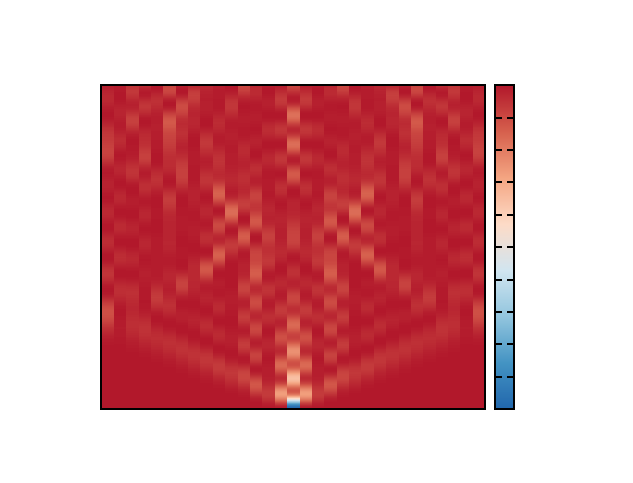
\includegraphics{Sz_l0_5}}%
    \gplfronttext
  \end{picture}%
\endgroup
}
        \caption{$\lambda=0.5$}
        \label{fig:testsingle6}
    \end{subfigure}
    \end{figure}
    \begin{figure}
        \ContinuedFloat
    \begin{subfigure}{.5\textwidth}
        \centering
        \resizebox{\textwidth}{!}{% GNUPLOT: LaTeX picture with Postscript
\begingroup
  \makeatletter
  \providecommand\color[2][]{%
    \GenericError{(gnuplot) \space\space\space\@spaces}{%
      Package color not loaded in conjunction with
      terminal option `colourtext'%
    }{See the gnuplot documentation for explanation.%
    }{Either use 'blacktext' in gnuplot or load the package
      color.sty in LaTeX.}%
    \renewcommand\color[2][]{}%
  }%
  \providecommand\includegraphics[2][]{%
    \GenericError{(gnuplot) \space\space\space\@spaces}{%
      Package graphicx or graphics not loaded%
    }{See the gnuplot documentation for explanation.%
    }{The gnuplot epslatex terminal needs graphicx.sty or graphics.sty.}%
    \renewcommand\includegraphics[2][]{}%
  }%
  \providecommand\rotatebox[2]{#2}%
  \@ifundefined{ifGPcolor}{%
    \newif\ifGPcolor
    \GPcolortrue
  }{}%
  \@ifundefined{ifGPblacktext}{%
    \newif\ifGPblacktext
    \GPblacktexttrue
  }{}%
  % define a \g@addto@macro without @ in the name:
  \let\gplgaddtomacro\g@addto@macro
  % define empty templates for all commands taking text:
  \gdef\gplbacktext{}%
  \gdef\gplfronttext{}%
  \makeatother
  \ifGPblacktext
    % no textcolor at all
    \def\colorrgb#1{}%
    \def\colorgray#1{}%
  \else
    % gray or color?
    \ifGPcolor
      \def\colorrgb#1{\color[rgb]{#1}}%
      \def\colorgray#1{\color[gray]{#1}}%
      \expandafter\def\csname LTw\endcsname{\color{white}}%
      \expandafter\def\csname LTb\endcsname{\color{black}}%
      \expandafter\def\csname LTa\endcsname{\color{black}}%
      \expandafter\def\csname LT0\endcsname{\color[rgb]{1,0,0}}%
      \expandafter\def\csname LT1\endcsname{\color[rgb]{0,1,0}}%
      \expandafter\def\csname LT2\endcsname{\color[rgb]{0,0,1}}%
      \expandafter\def\csname LT3\endcsname{\color[rgb]{1,0,1}}%
      \expandafter\def\csname LT4\endcsname{\color[rgb]{0,1,1}}%
      \expandafter\def\csname LT5\endcsname{\color[rgb]{1,1,0}}%
      \expandafter\def\csname LT6\endcsname{\color[rgb]{0,0,0}}%
      \expandafter\def\csname LT7\endcsname{\color[rgb]{1,0.3,0}}%
      \expandafter\def\csname LT8\endcsname{\color[rgb]{0.5,0.5,0.5}}%
    \else
      % gray
      \def\colorrgb#1{\color{black}}%
      \def\colorgray#1{\color[gray]{#1}}%
      \expandafter\def\csname LTw\endcsname{\color{white}}%
      \expandafter\def\csname LTb\endcsname{\color{black}}%
      \expandafter\def\csname LTa\endcsname{\color{black}}%
      \expandafter\def\csname LT0\endcsname{\color{black}}%
      \expandafter\def\csname LT1\endcsname{\color{black}}%
      \expandafter\def\csname LT2\endcsname{\color{black}}%
      \expandafter\def\csname LT3\endcsname{\color{black}}%
      \expandafter\def\csname LT4\endcsname{\color{black}}%
      \expandafter\def\csname LT5\endcsname{\color{black}}%
      \expandafter\def\csname LT6\endcsname{\color{black}}%
      \expandafter\def\csname LT7\endcsname{\color{black}}%
      \expandafter\def\csname LT8\endcsname{\color{black}}%
    \fi
  \fi
    \setlength{\unitlength}{0.0500bp}%
    \ifx\gptboxheight\undefined%
      \newlength{\gptboxheight}%
      \newlength{\gptboxwidth}%
      \newsavebox{\gptboxtext}%
    \fi%
    \setlength{\fboxrule}{0.5pt}%
    \setlength{\fboxsep}{1pt}%
\begin{picture}(5760.00,5760.00)%
    \gplgaddtomacro\gplbacktext{%
      \csname LTb\endcsname%
      \put(682,705){\makebox(0,0)[r]{\strut{}$0$}}%
      \put(682,1437){\makebox(0,0)[r]{\strut{}$5$}}%
      \put(682,2169){\makebox(0,0)[r]{\strut{}$10$}}%
      \put(682,2902){\makebox(0,0)[r]{\strut{}$15$}}%
      \put(682,3634){\makebox(0,0)[r]{\strut{}$20$}}%
      \put(682,4366){\makebox(0,0)[r]{\strut{}$25$}}%
      \put(682,5098){\makebox(0,0)[r]{\strut{}$30$}}%
      \put(873,484){\makebox(0,0){\strut{}$0$}}%
      \put(1468,484){\makebox(0,0){\strut{}$5$}}%
      \put(2062,484){\makebox(0,0){\strut{}$10$}}%
      \put(2656,484){\makebox(0,0){\strut{}$15$}}%
      \put(3250,484){\makebox(0,0){\strut{}$20$}}%
      \put(3844,484){\makebox(0,0){\strut{}$25$}}%
      \put(4439,484){\makebox(0,0){\strut{}$30$}}%
    }%
    \gplgaddtomacro\gplfronttext{%
      \csname LTb\endcsname%
      \put(176,2901){\rotatebox{-270}{\makebox(0,0){\strut{}time $t$}}}%
      \put(2656,154){\makebox(0,0){\strut{}particle index $i$}}%
      \put(2656,5429){\makebox(0,0){\strut{}$\mu=0,~\lambda=$0.6}}%
      \csname LTb\endcsname%
      \put(4906,704){\makebox(0,0)[l]{\strut{}$-0.5$}}%
      \put(4906,1143){\makebox(0,0)[l]{\strut{}$-0.4$}}%
      \put(4906,1583){\makebox(0,0)[l]{\strut{}$-0.3$}}%
      \put(4906,2022){\makebox(0,0)[l]{\strut{}$-0.2$}}%
      \put(4906,2462){\makebox(0,0)[l]{\strut{}$-0.1$}}%
      \put(4906,2901){\makebox(0,0)[l]{\strut{}$0$}}%
      \put(4906,3341){\makebox(0,0)[l]{\strut{}$0.1$}}%
      \put(4906,3780){\makebox(0,0)[l]{\strut{}$0.2$}}%
      \put(4906,4220){\makebox(0,0)[l]{\strut{}$0.3$}}%
      \put(4906,4659){\makebox(0,0)[l]{\strut{}$0.4$}}%
      \put(4906,5099){\makebox(0,0)[l]{\strut{}$0.5$}}%
      \put(5500,2901){\rotatebox{-270}{\makebox(0,0){\strut{}$\braket{S_1^z}_t$}}}%
    }%
    \gplbacktext
    \put(0,0){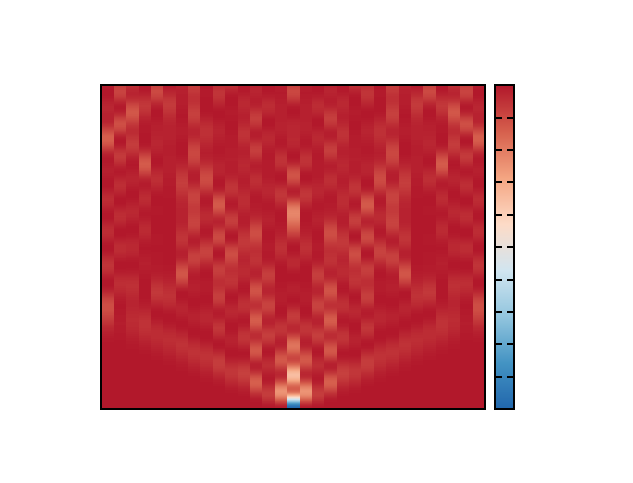
\includegraphics{Sz_l0_6}}%
    \gplfronttext
  \end{picture}%
\endgroup
}
        \caption{$\lambda=0.6$}
        \label{fig:testsingle7}
    \end{subfigure}
    \begin{subfigure}{.5\textwidth}
        \centering
        \resizebox{\textwidth}{!}{% GNUPLOT: LaTeX picture with Postscript
\begingroup
  \makeatletter
  \providecommand\color[2][]{%
    \GenericError{(gnuplot) \space\space\space\@spaces}{%
      Package color not loaded in conjunction with
      terminal option `colourtext'%
    }{See the gnuplot documentation for explanation.%
    }{Either use 'blacktext' in gnuplot or load the package
      color.sty in LaTeX.}%
    \renewcommand\color[2][]{}%
  }%
  \providecommand\includegraphics[2][]{%
    \GenericError{(gnuplot) \space\space\space\@spaces}{%
      Package graphicx or graphics not loaded%
    }{See the gnuplot documentation for explanation.%
    }{The gnuplot epslatex terminal needs graphicx.sty or graphics.sty.}%
    \renewcommand\includegraphics[2][]{}%
  }%
  \providecommand\rotatebox[2]{#2}%
  \@ifundefined{ifGPcolor}{%
    \newif\ifGPcolor
    \GPcolortrue
  }{}%
  \@ifundefined{ifGPblacktext}{%
    \newif\ifGPblacktext
    \GPblacktexttrue
  }{}%
  % define a \g@addto@macro without @ in the name:
  \let\gplgaddtomacro\g@addto@macro
  % define empty templates for all commands taking text:
  \gdef\gplbacktext{}%
  \gdef\gplfronttext{}%
  \makeatother
  \ifGPblacktext
    % no textcolor at all
    \def\colorrgb#1{}%
    \def\colorgray#1{}%
  \else
    % gray or color?
    \ifGPcolor
      \def\colorrgb#1{\color[rgb]{#1}}%
      \def\colorgray#1{\color[gray]{#1}}%
      \expandafter\def\csname LTw\endcsname{\color{white}}%
      \expandafter\def\csname LTb\endcsname{\color{black}}%
      \expandafter\def\csname LTa\endcsname{\color{black}}%
      \expandafter\def\csname LT0\endcsname{\color[rgb]{1,0,0}}%
      \expandafter\def\csname LT1\endcsname{\color[rgb]{0,1,0}}%
      \expandafter\def\csname LT2\endcsname{\color[rgb]{0,0,1}}%
      \expandafter\def\csname LT3\endcsname{\color[rgb]{1,0,1}}%
      \expandafter\def\csname LT4\endcsname{\color[rgb]{0,1,1}}%
      \expandafter\def\csname LT5\endcsname{\color[rgb]{1,1,0}}%
      \expandafter\def\csname LT6\endcsname{\color[rgb]{0,0,0}}%
      \expandafter\def\csname LT7\endcsname{\color[rgb]{1,0.3,0}}%
      \expandafter\def\csname LT8\endcsname{\color[rgb]{0.5,0.5,0.5}}%
    \else
      % gray
      \def\colorrgb#1{\color{black}}%
      \def\colorgray#1{\color[gray]{#1}}%
      \expandafter\def\csname LTw\endcsname{\color{white}}%
      \expandafter\def\csname LTb\endcsname{\color{black}}%
      \expandafter\def\csname LTa\endcsname{\color{black}}%
      \expandafter\def\csname LT0\endcsname{\color{black}}%
      \expandafter\def\csname LT1\endcsname{\color{black}}%
      \expandafter\def\csname LT2\endcsname{\color{black}}%
      \expandafter\def\csname LT3\endcsname{\color{black}}%
      \expandafter\def\csname LT4\endcsname{\color{black}}%
      \expandafter\def\csname LT5\endcsname{\color{black}}%
      \expandafter\def\csname LT6\endcsname{\color{black}}%
      \expandafter\def\csname LT7\endcsname{\color{black}}%
      \expandafter\def\csname LT8\endcsname{\color{black}}%
    \fi
  \fi
    \setlength{\unitlength}{0.0500bp}%
    \ifx\gptboxheight\undefined%
      \newlength{\gptboxheight}%
      \newlength{\gptboxwidth}%
      \newsavebox{\gptboxtext}%
    \fi%
    \setlength{\fboxrule}{0.5pt}%
    \setlength{\fboxsep}{1pt}%
\begin{picture}(5760.00,5760.00)%
    \gplgaddtomacro\gplbacktext{%
      \csname LTb\endcsname%
      \put(682,705){\makebox(0,0)[r]{\strut{}$0$}}%
      \put(682,1584){\makebox(0,0)[r]{\strut{}$5$}}%
      \put(682,2462){\makebox(0,0)[r]{\strut{}$10$}}%
      \put(682,3341){\makebox(0,0)[r]{\strut{}$15$}}%
      \put(682,4219){\makebox(0,0)[r]{\strut{}$20$}}%
      \put(682,5098){\makebox(0,0)[r]{\strut{}$25$}}%
      \put(873,484){\makebox(0,0){\strut{}$0$}}%
      \put(1468,484){\makebox(0,0){\strut{}$5$}}%
      \put(2062,484){\makebox(0,0){\strut{}$10$}}%
      \put(2656,484){\makebox(0,0){\strut{}$15$}}%
      \put(3250,484){\makebox(0,0){\strut{}$20$}}%
      \put(3844,484){\makebox(0,0){\strut{}$25$}}%
      \put(4439,484){\makebox(0,0){\strut{}$30$}}%
    }%
    \gplgaddtomacro\gplfronttext{%
      \csname LTb\endcsname%
      \put(176,2901){\rotatebox{-270}{\makebox(0,0){\strut{}time $t$}}}%
      \put(2656,154){\makebox(0,0){\strut{}particle index $i$}}%
      \put(2656,5429){\makebox(0,0){\strut{}$\mu=0,~\lambda=$0.7}}%
      \csname LTb\endcsname%
      \put(4906,704){\makebox(0,0)[l]{\strut{}$-0.5$}}%
      \put(4906,1143){\makebox(0,0)[l]{\strut{}$-0.4$}}%
      \put(4906,1583){\makebox(0,0)[l]{\strut{}$-0.3$}}%
      \put(4906,2022){\makebox(0,0)[l]{\strut{}$-0.2$}}%
      \put(4906,2462){\makebox(0,0)[l]{\strut{}$-0.1$}}%
      \put(4906,2901){\makebox(0,0)[l]{\strut{}$0$}}%
      \put(4906,3341){\makebox(0,0)[l]{\strut{}$0.1$}}%
      \put(4906,3780){\makebox(0,0)[l]{\strut{}$0.2$}}%
      \put(4906,4220){\makebox(0,0)[l]{\strut{}$0.3$}}%
      \put(4906,4659){\makebox(0,0)[l]{\strut{}$0.4$}}%
      \put(4906,5099){\makebox(0,0)[l]{\strut{}$0.5$}}%
      \put(5500,2901){\rotatebox{-270}{\makebox(0,0){\strut{}$\braket{S_1^z}_t$}}}%
    }%
    \gplbacktext
    \put(0,0){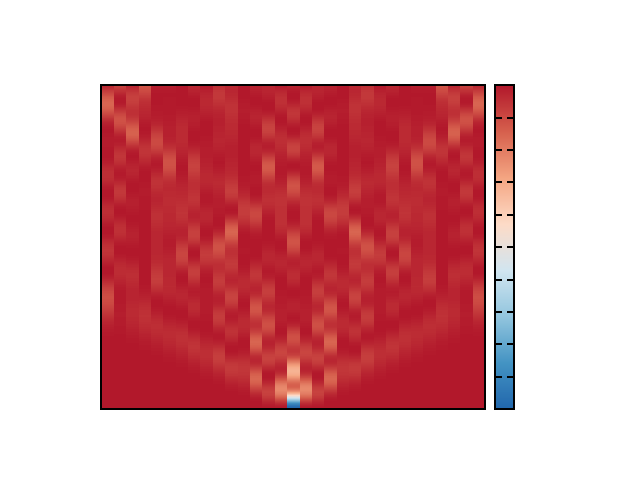
\includegraphics{Sz_l0_7}}%
    \gplfronttext
  \end{picture}%
\endgroup
}
        \caption{$\lambda=0.7$}
        \label{fig:testsingle8}
    \end{subfigure}
    \begin{subfigure}{.5\textwidth}
        \centering
        \resizebox{\textwidth}{!}{% GNUPLOT: LaTeX picture with Postscript
\begingroup
  \makeatletter
  \providecommand\color[2][]{%
    \GenericError{(gnuplot) \space\space\space\@spaces}{%
      Package color not loaded in conjunction with
      terminal option `colourtext'%
    }{See the gnuplot documentation for explanation.%
    }{Either use 'blacktext' in gnuplot or load the package
      color.sty in LaTeX.}%
    \renewcommand\color[2][]{}%
  }%
  \providecommand\includegraphics[2][]{%
    \GenericError{(gnuplot) \space\space\space\@spaces}{%
      Package graphicx or graphics not loaded%
    }{See the gnuplot documentation for explanation.%
    }{The gnuplot epslatex terminal needs graphicx.sty or graphics.sty.}%
    \renewcommand\includegraphics[2][]{}%
  }%
  \providecommand\rotatebox[2]{#2}%
  \@ifundefined{ifGPcolor}{%
    \newif\ifGPcolor
    \GPcolortrue
  }{}%
  \@ifundefined{ifGPblacktext}{%
    \newif\ifGPblacktext
    \GPblacktexttrue
  }{}%
  % define a \g@addto@macro without @ in the name:
  \let\gplgaddtomacro\g@addto@macro
  % define empty templates for all commands taking text:
  \gdef\gplbacktext{}%
  \gdef\gplfronttext{}%
  \makeatother
  \ifGPblacktext
    % no textcolor at all
    \def\colorrgb#1{}%
    \def\colorgray#1{}%
  \else
    % gray or color?
    \ifGPcolor
      \def\colorrgb#1{\color[rgb]{#1}}%
      \def\colorgray#1{\color[gray]{#1}}%
      \expandafter\def\csname LTw\endcsname{\color{white}}%
      \expandafter\def\csname LTb\endcsname{\color{black}}%
      \expandafter\def\csname LTa\endcsname{\color{black}}%
      \expandafter\def\csname LT0\endcsname{\color[rgb]{1,0,0}}%
      \expandafter\def\csname LT1\endcsname{\color[rgb]{0,1,0}}%
      \expandafter\def\csname LT2\endcsname{\color[rgb]{0,0,1}}%
      \expandafter\def\csname LT3\endcsname{\color[rgb]{1,0,1}}%
      \expandafter\def\csname LT4\endcsname{\color[rgb]{0,1,1}}%
      \expandafter\def\csname LT5\endcsname{\color[rgb]{1,1,0}}%
      \expandafter\def\csname LT6\endcsname{\color[rgb]{0,0,0}}%
      \expandafter\def\csname LT7\endcsname{\color[rgb]{1,0.3,0}}%
      \expandafter\def\csname LT8\endcsname{\color[rgb]{0.5,0.5,0.5}}%
    \else
      % gray
      \def\colorrgb#1{\color{black}}%
      \def\colorgray#1{\color[gray]{#1}}%
      \expandafter\def\csname LTw\endcsname{\color{white}}%
      \expandafter\def\csname LTb\endcsname{\color{black}}%
      \expandafter\def\csname LTa\endcsname{\color{black}}%
      \expandafter\def\csname LT0\endcsname{\color{black}}%
      \expandafter\def\csname LT1\endcsname{\color{black}}%
      \expandafter\def\csname LT2\endcsname{\color{black}}%
      \expandafter\def\csname LT3\endcsname{\color{black}}%
      \expandafter\def\csname LT4\endcsname{\color{black}}%
      \expandafter\def\csname LT5\endcsname{\color{black}}%
      \expandafter\def\csname LT6\endcsname{\color{black}}%
      \expandafter\def\csname LT7\endcsname{\color{black}}%
      \expandafter\def\csname LT8\endcsname{\color{black}}%
    \fi
  \fi
    \setlength{\unitlength}{0.0500bp}%
    \ifx\gptboxheight\undefined%
      \newlength{\gptboxheight}%
      \newlength{\gptboxwidth}%
      \newsavebox{\gptboxtext}%
    \fi%
    \setlength{\fboxrule}{0.5pt}%
    \setlength{\fboxsep}{1pt}%
\begin{picture}(5760.00,4320.00)%
    \gplgaddtomacro\gplbacktext{%
      \csname LTb\endcsname%
      \put(682,551){\makebox(0,0)[r]{\strut{}$0$}}%
      \put(682,1328){\makebox(0,0)[r]{\strut{}$5$}}%
      \put(682,2105){\makebox(0,0)[r]{\strut{}$10$}}%
      \put(682,2881){\makebox(0,0)[r]{\strut{}$15$}}%
      \put(682,3658){\makebox(0,0)[r]{\strut{}$20$}}%
      \put(873,330){\makebox(0,0){\strut{}$0$}}%
      \put(1468,330){\makebox(0,0){\strut{}$5$}}%
      \put(2062,330){\makebox(0,0){\strut{}$10$}}%
      \put(2656,330){\makebox(0,0){\strut{}$15$}}%
      \put(3250,330){\makebox(0,0){\strut{}$20$}}%
      \put(3844,330){\makebox(0,0){\strut{}$25$}}%
      \put(4439,330){\makebox(0,0){\strut{}$30$}}%
    }%
    \gplgaddtomacro\gplfronttext{%
      \csname LTb\endcsname%
      \put(176,2104){\rotatebox{-270}{\makebox(0,0){\strut{}time $Jt$}}}%
      \put(2656,0){\makebox(0,0){\strut{}particle index $i$}}%
      \put(2656,3989){\makebox(0,0){\strut{}$\mu=0,~\lambda=$0.8~$N=31$}}%
      \csname LTb\endcsname%
      \put(4906,550){\makebox(0,0)[l]{\strut{}$-0.5$}}%
      \put(4906,860){\makebox(0,0)[l]{\strut{}$-0.4$}}%
      \put(4906,1171){\makebox(0,0)[l]{\strut{}$-0.3$}}%
      \put(4906,1482){\makebox(0,0)[l]{\strut{}$-0.2$}}%
      \put(4906,1793){\makebox(0,0)[l]{\strut{}$-0.1$}}%
      \put(4906,2104){\makebox(0,0)[l]{\strut{}$0$}}%
      \put(4906,2415){\makebox(0,0)[l]{\strut{}$0.1$}}%
      \put(4906,2726){\makebox(0,0)[l]{\strut{}$0.2$}}%
      \put(4906,3037){\makebox(0,0)[l]{\strut{}$0.3$}}%
      \put(4906,3348){\makebox(0,0)[l]{\strut{}$0.4$}}%
      \put(4906,3659){\makebox(0,0)[l]{\strut{}$0.5$}}%
      \put(5500,2104){\rotatebox{-270}{\makebox(0,0){\strut{}$\braket{S_1^z}_t$}}}%
    }%
    \gplbacktext
    \put(0,0){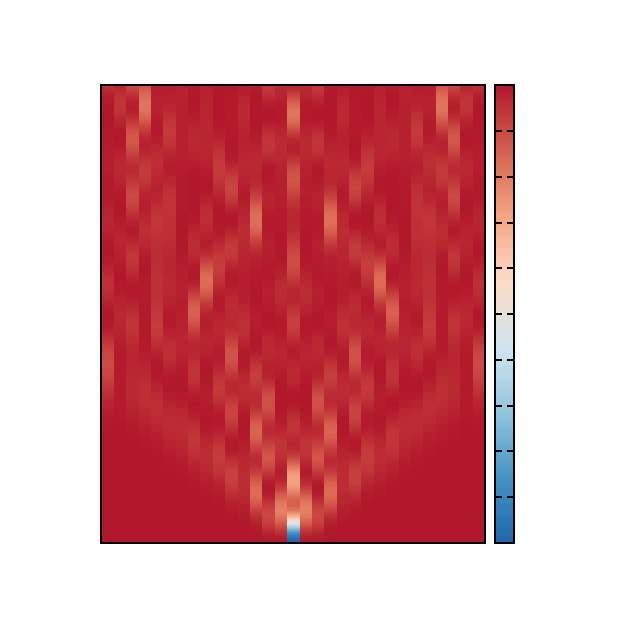
\includegraphics{Sz_l0_8}}%
    \gplfronttext
  \end{picture}%
\endgroup
}
        \caption{$\lambda=0.8$}
        \label{fig:testsingle9}
    \end{subfigure}
    \begin{subfigure}{.5\textwidth}
        \centering
        \resizebox{\textwidth}{!}{% GNUPLOT: LaTeX picture with Postscript
\begingroup
  \makeatletter
  \providecommand\color[2][]{%
    \GenericError{(gnuplot) \space\space\space\@spaces}{%
      Package color not loaded in conjunction with
      terminal option `colourtext'%
    }{See the gnuplot documentation for explanation.%
    }{Either use 'blacktext' in gnuplot or load the package
      color.sty in LaTeX.}%
    \renewcommand\color[2][]{}%
  }%
  \providecommand\includegraphics[2][]{%
    \GenericError{(gnuplot) \space\space\space\@spaces}{%
      Package graphicx or graphics not loaded%
    }{See the gnuplot documentation for explanation.%
    }{The gnuplot epslatex terminal needs graphicx.sty or graphics.sty.}%
    \renewcommand\includegraphics[2][]{}%
  }%
  \providecommand\rotatebox[2]{#2}%
  \@ifundefined{ifGPcolor}{%
    \newif\ifGPcolor
    \GPcolortrue
  }{}%
  \@ifundefined{ifGPblacktext}{%
    \newif\ifGPblacktext
    \GPblacktexttrue
  }{}%
  % define a \g@addto@macro without @ in the name:
  \let\gplgaddtomacro\g@addto@macro
  % define empty templates for all commands taking text:
  \gdef\gplbacktext{}%
  \gdef\gplfronttext{}%
  \makeatother
  \ifGPblacktext
    % no textcolor at all
    \def\colorrgb#1{}%
    \def\colorgray#1{}%
  \else
    % gray or color?
    \ifGPcolor
      \def\colorrgb#1{\color[rgb]{#1}}%
      \def\colorgray#1{\color[gray]{#1}}%
      \expandafter\def\csname LTw\endcsname{\color{white}}%
      \expandafter\def\csname LTb\endcsname{\color{black}}%
      \expandafter\def\csname LTa\endcsname{\color{black}}%
      \expandafter\def\csname LT0\endcsname{\color[rgb]{1,0,0}}%
      \expandafter\def\csname LT1\endcsname{\color[rgb]{0,1,0}}%
      \expandafter\def\csname LT2\endcsname{\color[rgb]{0,0,1}}%
      \expandafter\def\csname LT3\endcsname{\color[rgb]{1,0,1}}%
      \expandafter\def\csname LT4\endcsname{\color[rgb]{0,1,1}}%
      \expandafter\def\csname LT5\endcsname{\color[rgb]{1,1,0}}%
      \expandafter\def\csname LT6\endcsname{\color[rgb]{0,0,0}}%
      \expandafter\def\csname LT7\endcsname{\color[rgb]{1,0.3,0}}%
      \expandafter\def\csname LT8\endcsname{\color[rgb]{0.5,0.5,0.5}}%
    \else
      % gray
      \def\colorrgb#1{\color{black}}%
      \def\colorgray#1{\color[gray]{#1}}%
      \expandafter\def\csname LTw\endcsname{\color{white}}%
      \expandafter\def\csname LTb\endcsname{\color{black}}%
      \expandafter\def\csname LTa\endcsname{\color{black}}%
      \expandafter\def\csname LT0\endcsname{\color{black}}%
      \expandafter\def\csname LT1\endcsname{\color{black}}%
      \expandafter\def\csname LT2\endcsname{\color{black}}%
      \expandafter\def\csname LT3\endcsname{\color{black}}%
      \expandafter\def\csname LT4\endcsname{\color{black}}%
      \expandafter\def\csname LT5\endcsname{\color{black}}%
      \expandafter\def\csname LT6\endcsname{\color{black}}%
      \expandafter\def\csname LT7\endcsname{\color{black}}%
      \expandafter\def\csname LT8\endcsname{\color{black}}%
    \fi
  \fi
    \setlength{\unitlength}{0.0500bp}%
    \ifx\gptboxheight\undefined%
      \newlength{\gptboxheight}%
      \newlength{\gptboxwidth}%
      \newsavebox{\gptboxtext}%
    \fi%
    \setlength{\fboxrule}{0.5pt}%
    \setlength{\fboxsep}{1pt}%
\begin{picture}(5760.00,5760.00)%
    \gplgaddtomacro\gplbacktext{%
      \csname LTb\endcsname%
      \put(682,705){\makebox(0,0)[r]{\strut{}$0$}}%
      \put(682,1291){\makebox(0,0)[r]{\strut{}$2$}}%
      \put(682,1876){\makebox(0,0)[r]{\strut{}$4$}}%
      \put(682,2461){\makebox(0,0)[r]{\strut{}$6$}}%
      \put(682,3046){\makebox(0,0)[r]{\strut{}$8$}}%
      \put(682,3632){\makebox(0,0)[r]{\strut{}$10$}}%
      \put(682,4217){\makebox(0,0)[r]{\strut{}$12$}}%
      \put(682,4802){\makebox(0,0)[r]{\strut{}$14$}}%
      \put(873,484){\makebox(0,0){\strut{}$0$}}%
      \put(1468,484){\makebox(0,0){\strut{}$5$}}%
      \put(2062,484){\makebox(0,0){\strut{}$10$}}%
      \put(2656,484){\makebox(0,0){\strut{}$15$}}%
      \put(3250,484){\makebox(0,0){\strut{}$20$}}%
      \put(3844,484){\makebox(0,0){\strut{}$25$}}%
      \put(4439,484){\makebox(0,0){\strut{}$30$}}%
    }%
    \gplgaddtomacro\gplfronttext{%
      \csname LTb\endcsname%
      \put(176,2901){\rotatebox{-270}{\makebox(0,0){\strut{}time $t$}}}%
      \put(2656,154){\makebox(0,0){\strut{}particle index $i$}}%
      \put(2656,5429){\makebox(0,0){\strut{}$\mu=0,~\lambda=$0.9}}%
      \csname LTb\endcsname%
      \put(4906,704){\makebox(0,0)[l]{\strut{}$-0.5$}}%
      \put(4906,1143){\makebox(0,0)[l]{\strut{}$-0.4$}}%
      \put(4906,1583){\makebox(0,0)[l]{\strut{}$-0.3$}}%
      \put(4906,2022){\makebox(0,0)[l]{\strut{}$-0.2$}}%
      \put(4906,2462){\makebox(0,0)[l]{\strut{}$-0.1$}}%
      \put(4906,2901){\makebox(0,0)[l]{\strut{}$0$}}%
      \put(4906,3341){\makebox(0,0)[l]{\strut{}$0.1$}}%
      \put(4906,3780){\makebox(0,0)[l]{\strut{}$0.2$}}%
      \put(4906,4220){\makebox(0,0)[l]{\strut{}$0.3$}}%
      \put(4906,4659){\makebox(0,0)[l]{\strut{}$0.4$}}%
      \put(4906,5099){\makebox(0,0)[l]{\strut{}$0.5$}}%
      \put(5500,2901){\rotatebox{-270}{\makebox(0,0){\strut{}$\braket{S_1^z}_t$}}}%
    }%
    \gplbacktext
    \put(0,0){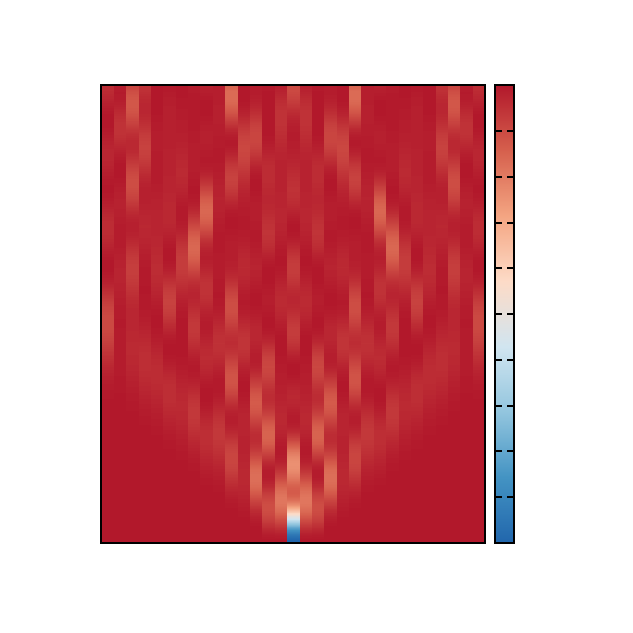
\includegraphics{Sz_l0_9}}%
    \gplfronttext
  \end{picture}%
\endgroup
}
        \caption{$\lambda=0.9$}
        \label{fig:testsingle10}
    \end{subfigure}
    \caption{Space time plot of the Propagation of single spin excitations in the form of magnons depending on the NNN coupling parameter $\lambda$.}
\end{figure}
\subsection{Multiple-string magnon propagation}
This time, we consider a double spin flip in the middle as the initial state:
\begin{align}
    \ket a =\ket{\uparrow\uparrow\dots\uparrow\uparrow\downarrow\downarrow\uparrow\uparrow\dots\uparrow\uparrow}.
    \label{eq:initdouble}
\end{align}
The space time plot for $N=30$ and $\lambda=0$ and varying $\mu$ is shown in \cref{fig:testdouble1,fig:testdouble2,fig:testdouble3,fig:testdouble4,fig:testdouble5,fig:testdouble6,fig:testdouble7,fig:testdouble8,fig:testdouble9,fig:testdouble10}. For low $\mu$ the qualitative behaviour mirrors that of the previous section. However, when increasing $\mu$, a second, slower propagation cascade is developing and eventually ovepowering the original cascade. This is in agreement to \cite{ganahlpaper} and is explained by the formation of bound states between two spins, so called ``two-string magnons''. The higher $\mu$, the stronger these spins are bound together and the slower they propagate.

\begin{figure}[]
    \begin{subfigure}{.5\textwidth}
        \centering
        \resizebox{\textwidth}{!}{% GNUPLOT: LaTeX picture with Postscript
\begingroup
  \makeatletter
  \providecommand\color[2][]{%
    \GenericError{(gnuplot) \space\space\space\@spaces}{%
      Package color not loaded in conjunction with
      terminal option `colourtext'%
    }{See the gnuplot documentation for explanation.%
    }{Either use 'blacktext' in gnuplot or load the package
      color.sty in LaTeX.}%
    \renewcommand\color[2][]{}%
  }%
  \providecommand\includegraphics[2][]{%
    \GenericError{(gnuplot) \space\space\space\@spaces}{%
      Package graphicx or graphics not loaded%
    }{See the gnuplot documentation for explanation.%
    }{The gnuplot epslatex terminal needs graphicx.sty or graphics.sty.}%
    \renewcommand\includegraphics[2][]{}%
  }%
  \providecommand\rotatebox[2]{#2}%
  \@ifundefined{ifGPcolor}{%
    \newif\ifGPcolor
    \GPcolortrue
  }{}%
  \@ifundefined{ifGPblacktext}{%
    \newif\ifGPblacktext
    \GPblacktexttrue
  }{}%
  % define a \g@addto@macro without @ in the name:
  \let\gplgaddtomacro\g@addto@macro
  % define empty templates for all commands taking text:
  \gdef\gplbacktext{}%
  \gdef\gplfronttext{}%
  \makeatother
  \ifGPblacktext
    % no textcolor at all
    \def\colorrgb#1{}%
    \def\colorgray#1{}%
  \else
    % gray or color?
    \ifGPcolor
      \def\colorrgb#1{\color[rgb]{#1}}%
      \def\colorgray#1{\color[gray]{#1}}%
      \expandafter\def\csname LTw\endcsname{\color{white}}%
      \expandafter\def\csname LTb\endcsname{\color{black}}%
      \expandafter\def\csname LTa\endcsname{\color{black}}%
      \expandafter\def\csname LT0\endcsname{\color[rgb]{1,0,0}}%
      \expandafter\def\csname LT1\endcsname{\color[rgb]{0,1,0}}%
      \expandafter\def\csname LT2\endcsname{\color[rgb]{0,0,1}}%
      \expandafter\def\csname LT3\endcsname{\color[rgb]{1,0,1}}%
      \expandafter\def\csname LT4\endcsname{\color[rgb]{0,1,1}}%
      \expandafter\def\csname LT5\endcsname{\color[rgb]{1,1,0}}%
      \expandafter\def\csname LT6\endcsname{\color[rgb]{0,0,0}}%
      \expandafter\def\csname LT7\endcsname{\color[rgb]{1,0.3,0}}%
      \expandafter\def\csname LT8\endcsname{\color[rgb]{0.5,0.5,0.5}}%
    \else
      % gray
      \def\colorrgb#1{\color{black}}%
      \def\colorgray#1{\color[gray]{#1}}%
      \expandafter\def\csname LTw\endcsname{\color{white}}%
      \expandafter\def\csname LTb\endcsname{\color{black}}%
      \expandafter\def\csname LTa\endcsname{\color{black}}%
      \expandafter\def\csname LT0\endcsname{\color{black}}%
      \expandafter\def\csname LT1\endcsname{\color{black}}%
      \expandafter\def\csname LT2\endcsname{\color{black}}%
      \expandafter\def\csname LT3\endcsname{\color{black}}%
      \expandafter\def\csname LT4\endcsname{\color{black}}%
      \expandafter\def\csname LT5\endcsname{\color{black}}%
      \expandafter\def\csname LT6\endcsname{\color{black}}%
      \expandafter\def\csname LT7\endcsname{\color{black}}%
      \expandafter\def\csname LT8\endcsname{\color{black}}%
    \fi
  \fi
    \setlength{\unitlength}{0.0500bp}%
    \ifx\gptboxheight\undefined%
      \newlength{\gptboxheight}%
      \newlength{\gptboxwidth}%
      \newsavebox{\gptboxtext}%
    \fi%
    \setlength{\fboxrule}{0.5pt}%
    \setlength{\fboxsep}{1pt}%
\begin{picture}(5760.00,4320.00)%
    \gplgaddtomacro\gplbacktext{%
      \csname LTb\endcsname%
      \put(682,551){\makebox(0,0)[r]{\strut{}$0$}}%
      \put(682,1069){\makebox(0,0)[r]{\strut{}$10$}}%
      \put(682,1587){\makebox(0,0)[r]{\strut{}$20$}}%
      \put(682,2105){\makebox(0,0)[r]{\strut{}$30$}}%
      \put(682,2622){\makebox(0,0)[r]{\strut{}$40$}}%
      \put(682,3140){\makebox(0,0)[r]{\strut{}$50$}}%
      \put(682,3658){\makebox(0,0)[r]{\strut{}$60$}}%
      \put(875,330){\makebox(0,0){\strut{}$0$}}%
      \put(1489,330){\makebox(0,0){\strut{}$5$}}%
      \put(2103,330){\makebox(0,0){\strut{}$10$}}%
      \put(2717,330){\makebox(0,0){\strut{}$15$}}%
      \put(3331,330){\makebox(0,0){\strut{}$20$}}%
      \put(3945,330){\makebox(0,0){\strut{}$25$}}%
    }%
    \gplgaddtomacro\gplfronttext{%
      \csname LTb\endcsname%
      \put(176,2104){\rotatebox{-270}{\makebox(0,0){\strut{}time $Jt$}}}%
      \put(2656,0){\makebox(0,0){\strut{}particle index $i$}}%
      \put(2656,3989){\makebox(0,0){\strut{}$\lambda=0,~\mu=$0.0,~$N=30$}}%
      \csname LTb\endcsname%
      \put(4906,550){\makebox(0,0)[l]{\strut{}$-0.5$}}%
      \put(4906,860){\makebox(0,0)[l]{\strut{}$-0.4$}}%
      \put(4906,1171){\makebox(0,0)[l]{\strut{}$-0.3$}}%
      \put(4906,1482){\makebox(0,0)[l]{\strut{}$-0.2$}}%
      \put(4906,1793){\makebox(0,0)[l]{\strut{}$-0.1$}}%
      \put(4906,2104){\makebox(0,0)[l]{\strut{}$0$}}%
      \put(4906,2415){\makebox(0,0)[l]{\strut{}$0.1$}}%
      \put(4906,2726){\makebox(0,0)[l]{\strut{}$0.2$}}%
      \put(4906,3037){\makebox(0,0)[l]{\strut{}$0.3$}}%
      \put(4906,3348){\makebox(0,0)[l]{\strut{}$0.4$}}%
      \put(4906,3659){\makebox(0,0)[l]{\strut{}$0.5$}}%
      \put(5500,2104){\rotatebox{-270}{\makebox(0,0){\strut{}$\braket{S_1^z}_t$}}}%
    }%
    \gplbacktext
    \put(0,0){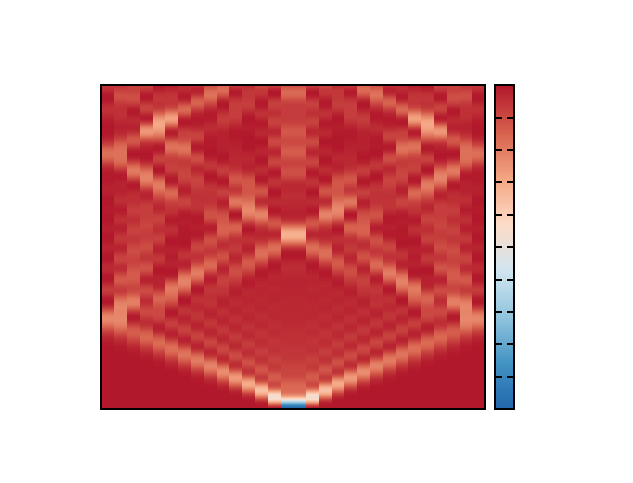
\includegraphics{Sz2_l0_mu0_0}}%
    \gplfronttext
  \end{picture}%
\endgroup
}
        \caption{$\mu=0$}
        \label{fig:testdouble1}
    \end{subfigure}
    \begin{subfigure}{.5\textwidth}
        \centering
        \resizebox{\textwidth}{!}{% GNUPLOT: LaTeX picture with Postscript
\begingroup
  \makeatletter
  \providecommand\color[2][]{%
    \GenericError{(gnuplot) \space\space\space\@spaces}{%
      Package color not loaded in conjunction with
      terminal option `colourtext'%
    }{See the gnuplot documentation for explanation.%
    }{Either use 'blacktext' in gnuplot or load the package
      color.sty in LaTeX.}%
    \renewcommand\color[2][]{}%
  }%
  \providecommand\includegraphics[2][]{%
    \GenericError{(gnuplot) \space\space\space\@spaces}{%
      Package graphicx or graphics not loaded%
    }{See the gnuplot documentation for explanation.%
    }{The gnuplot epslatex terminal needs graphicx.sty or graphics.sty.}%
    \renewcommand\includegraphics[2][]{}%
  }%
  \providecommand\rotatebox[2]{#2}%
  \@ifundefined{ifGPcolor}{%
    \newif\ifGPcolor
    \GPcolortrue
  }{}%
  \@ifundefined{ifGPblacktext}{%
    \newif\ifGPblacktext
    \GPblacktexttrue
  }{}%
  % define a \g@addto@macro without @ in the name:
  \let\gplgaddtomacro\g@addto@macro
  % define empty templates for all commands taking text:
  \gdef\gplbacktext{}%
  \gdef\gplfronttext{}%
  \makeatother
  \ifGPblacktext
    % no textcolor at all
    \def\colorrgb#1{}%
    \def\colorgray#1{}%
  \else
    % gray or color?
    \ifGPcolor
      \def\colorrgb#1{\color[rgb]{#1}}%
      \def\colorgray#1{\color[gray]{#1}}%
      \expandafter\def\csname LTw\endcsname{\color{white}}%
      \expandafter\def\csname LTb\endcsname{\color{black}}%
      \expandafter\def\csname LTa\endcsname{\color{black}}%
      \expandafter\def\csname LT0\endcsname{\color[rgb]{1,0,0}}%
      \expandafter\def\csname LT1\endcsname{\color[rgb]{0,1,0}}%
      \expandafter\def\csname LT2\endcsname{\color[rgb]{0,0,1}}%
      \expandafter\def\csname LT3\endcsname{\color[rgb]{1,0,1}}%
      \expandafter\def\csname LT4\endcsname{\color[rgb]{0,1,1}}%
      \expandafter\def\csname LT5\endcsname{\color[rgb]{1,1,0}}%
      \expandafter\def\csname LT6\endcsname{\color[rgb]{0,0,0}}%
      \expandafter\def\csname LT7\endcsname{\color[rgb]{1,0.3,0}}%
      \expandafter\def\csname LT8\endcsname{\color[rgb]{0.5,0.5,0.5}}%
    \else
      % gray
      \def\colorrgb#1{\color{black}}%
      \def\colorgray#1{\color[gray]{#1}}%
      \expandafter\def\csname LTw\endcsname{\color{white}}%
      \expandafter\def\csname LTb\endcsname{\color{black}}%
      \expandafter\def\csname LTa\endcsname{\color{black}}%
      \expandafter\def\csname LT0\endcsname{\color{black}}%
      \expandafter\def\csname LT1\endcsname{\color{black}}%
      \expandafter\def\csname LT2\endcsname{\color{black}}%
      \expandafter\def\csname LT3\endcsname{\color{black}}%
      \expandafter\def\csname LT4\endcsname{\color{black}}%
      \expandafter\def\csname LT5\endcsname{\color{black}}%
      \expandafter\def\csname LT6\endcsname{\color{black}}%
      \expandafter\def\csname LT7\endcsname{\color{black}}%
      \expandafter\def\csname LT8\endcsname{\color{black}}%
    \fi
  \fi
    \setlength{\unitlength}{0.0500bp}%
    \ifx\gptboxheight\undefined%
      \newlength{\gptboxheight}%
      \newlength{\gptboxwidth}%
      \newsavebox{\gptboxtext}%
    \fi%
    \setlength{\fboxrule}{0.5pt}%
    \setlength{\fboxsep}{1pt}%
\begin{picture}(5760.00,4320.00)%
    \gplgaddtomacro\gplbacktext{%
      \csname LTb\endcsname%
      \put(682,551){\makebox(0,0)[r]{\strut{}$0$}}%
      \put(682,1069){\makebox(0,0)[r]{\strut{}$10$}}%
      \put(682,1587){\makebox(0,0)[r]{\strut{}$20$}}%
      \put(682,2105){\makebox(0,0)[r]{\strut{}$30$}}%
      \put(682,2622){\makebox(0,0)[r]{\strut{}$40$}}%
      \put(682,3140){\makebox(0,0)[r]{\strut{}$50$}}%
      \put(682,3658){\makebox(0,0)[r]{\strut{}$60$}}%
      \put(875,330){\makebox(0,0){\strut{}$0$}}%
      \put(1489,330){\makebox(0,0){\strut{}$5$}}%
      \put(2103,330){\makebox(0,0){\strut{}$10$}}%
      \put(2717,330){\makebox(0,0){\strut{}$15$}}%
      \put(3331,330){\makebox(0,0){\strut{}$20$}}%
      \put(3945,330){\makebox(0,0){\strut{}$25$}}%
    }%
    \gplgaddtomacro\gplfronttext{%
      \csname LTb\endcsname%
      \put(176,2104){\rotatebox{-270}{\makebox(0,0){\strut{}time $Jt$}}}%
      \put(2656,0){\makebox(0,0){\strut{}particle index $i$}}%
      \put(2656,3989){\makebox(0,0){\strut{}$\lambda=0,~\mu=$0.1,~$N=30$}}%
      \csname LTb\endcsname%
      \put(4906,550){\makebox(0,0)[l]{\strut{}$-0.5$}}%
      \put(4906,860){\makebox(0,0)[l]{\strut{}$-0.4$}}%
      \put(4906,1171){\makebox(0,0)[l]{\strut{}$-0.3$}}%
      \put(4906,1482){\makebox(0,0)[l]{\strut{}$-0.2$}}%
      \put(4906,1793){\makebox(0,0)[l]{\strut{}$-0.1$}}%
      \put(4906,2104){\makebox(0,0)[l]{\strut{}$0$}}%
      \put(4906,2415){\makebox(0,0)[l]{\strut{}$0.1$}}%
      \put(4906,2726){\makebox(0,0)[l]{\strut{}$0.2$}}%
      \put(4906,3037){\makebox(0,0)[l]{\strut{}$0.3$}}%
      \put(4906,3348){\makebox(0,0)[l]{\strut{}$0.4$}}%
      \put(4906,3659){\makebox(0,0)[l]{\strut{}$0.5$}}%
      \put(5500,2104){\rotatebox{-270}{\makebox(0,0){\strut{}$\braket{S_1^z}_t$}}}%
    }%
    \gplbacktext
    \put(0,0){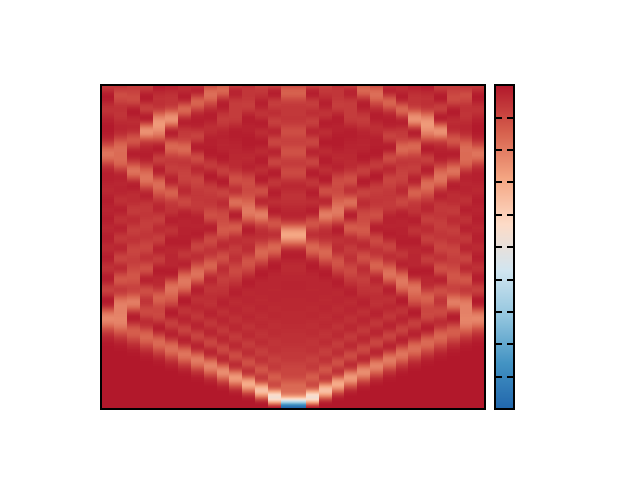
\includegraphics{Sz2_l0_mu0_1}}%
    \gplfronttext
  \end{picture}%
\endgroup
}
        \caption{$\mu=0.1$}
        \label{fig:testdouble2}
    \end{subfigure}
    \begin{subfigure}{.5\textwidth}
        \centering
        \resizebox{\textwidth}{!}{% GNUPLOT: LaTeX picture with Postscript
\begingroup
  \makeatletter
  \providecommand\color[2][]{%
    \GenericError{(gnuplot) \space\space\space\@spaces}{%
      Package color not loaded in conjunction with
      terminal option `colourtext'%
    }{See the gnuplot documentation for explanation.%
    }{Either use 'blacktext' in gnuplot or load the package
      color.sty in LaTeX.}%
    \renewcommand\color[2][]{}%
  }%
  \providecommand\includegraphics[2][]{%
    \GenericError{(gnuplot) \space\space\space\@spaces}{%
      Package graphicx or graphics not loaded%
    }{See the gnuplot documentation for explanation.%
    }{The gnuplot epslatex terminal needs graphicx.sty or graphics.sty.}%
    \renewcommand\includegraphics[2][]{}%
  }%
  \providecommand\rotatebox[2]{#2}%
  \@ifundefined{ifGPcolor}{%
    \newif\ifGPcolor
    \GPcolortrue
  }{}%
  \@ifundefined{ifGPblacktext}{%
    \newif\ifGPblacktext
    \GPblacktexttrue
  }{}%
  % define a \g@addto@macro without @ in the name:
  \let\gplgaddtomacro\g@addto@macro
  % define empty templates for all commands taking text:
  \gdef\gplbacktext{}%
  \gdef\gplfronttext{}%
  \makeatother
  \ifGPblacktext
    % no textcolor at all
    \def\colorrgb#1{}%
    \def\colorgray#1{}%
  \else
    % gray or color?
    \ifGPcolor
      \def\colorrgb#1{\color[rgb]{#1}}%
      \def\colorgray#1{\color[gray]{#1}}%
      \expandafter\def\csname LTw\endcsname{\color{white}}%
      \expandafter\def\csname LTb\endcsname{\color{black}}%
      \expandafter\def\csname LTa\endcsname{\color{black}}%
      \expandafter\def\csname LT0\endcsname{\color[rgb]{1,0,0}}%
      \expandafter\def\csname LT1\endcsname{\color[rgb]{0,1,0}}%
      \expandafter\def\csname LT2\endcsname{\color[rgb]{0,0,1}}%
      \expandafter\def\csname LT3\endcsname{\color[rgb]{1,0,1}}%
      \expandafter\def\csname LT4\endcsname{\color[rgb]{0,1,1}}%
      \expandafter\def\csname LT5\endcsname{\color[rgb]{1,1,0}}%
      \expandafter\def\csname LT6\endcsname{\color[rgb]{0,0,0}}%
      \expandafter\def\csname LT7\endcsname{\color[rgb]{1,0.3,0}}%
      \expandafter\def\csname LT8\endcsname{\color[rgb]{0.5,0.5,0.5}}%
    \else
      % gray
      \def\colorrgb#1{\color{black}}%
      \def\colorgray#1{\color[gray]{#1}}%
      \expandafter\def\csname LTw\endcsname{\color{white}}%
      \expandafter\def\csname LTb\endcsname{\color{black}}%
      \expandafter\def\csname LTa\endcsname{\color{black}}%
      \expandafter\def\csname LT0\endcsname{\color{black}}%
      \expandafter\def\csname LT1\endcsname{\color{black}}%
      \expandafter\def\csname LT2\endcsname{\color{black}}%
      \expandafter\def\csname LT3\endcsname{\color{black}}%
      \expandafter\def\csname LT4\endcsname{\color{black}}%
      \expandafter\def\csname LT5\endcsname{\color{black}}%
      \expandafter\def\csname LT6\endcsname{\color{black}}%
      \expandafter\def\csname LT7\endcsname{\color{black}}%
      \expandafter\def\csname LT8\endcsname{\color{black}}%
    \fi
  \fi
    \setlength{\unitlength}{0.0500bp}%
    \ifx\gptboxheight\undefined%
      \newlength{\gptboxheight}%
      \newlength{\gptboxwidth}%
      \newsavebox{\gptboxtext}%
    \fi%
    \setlength{\fboxrule}{0.5pt}%
    \setlength{\fboxsep}{1pt}%
\begin{picture}(5760.00,4320.00)%
    \gplgaddtomacro\gplbacktext{%
      \csname LTb\endcsname%
      \put(682,551){\makebox(0,0)[r]{\strut{}$0$}}%
      \put(682,1069){\makebox(0,0)[r]{\strut{}$10$}}%
      \put(682,1587){\makebox(0,0)[r]{\strut{}$20$}}%
      \put(682,2105){\makebox(0,0)[r]{\strut{}$30$}}%
      \put(682,2622){\makebox(0,0)[r]{\strut{}$40$}}%
      \put(682,3140){\makebox(0,0)[r]{\strut{}$50$}}%
      \put(682,3658){\makebox(0,0)[r]{\strut{}$60$}}%
      \put(875,330){\makebox(0,0){\strut{}$0$}}%
      \put(1489,330){\makebox(0,0){\strut{}$5$}}%
      \put(2103,330){\makebox(0,0){\strut{}$10$}}%
      \put(2717,330){\makebox(0,0){\strut{}$15$}}%
      \put(3331,330){\makebox(0,0){\strut{}$20$}}%
      \put(3945,330){\makebox(0,0){\strut{}$25$}}%
    }%
    \gplgaddtomacro\gplfronttext{%
      \csname LTb\endcsname%
      \put(176,2104){\rotatebox{-270}{\makebox(0,0){\strut{}time $Jt$}}}%
      \put(2656,0){\makebox(0,0){\strut{}particle index $i$}}%
      \put(2656,3989){\makebox(0,0){\strut{}$\lambda=0,~\mu=$0.2,~$N=30$}}%
      \csname LTb\endcsname%
      \put(4906,550){\makebox(0,0)[l]{\strut{}$-0.5$}}%
      \put(4906,860){\makebox(0,0)[l]{\strut{}$-0.4$}}%
      \put(4906,1171){\makebox(0,0)[l]{\strut{}$-0.3$}}%
      \put(4906,1482){\makebox(0,0)[l]{\strut{}$-0.2$}}%
      \put(4906,1793){\makebox(0,0)[l]{\strut{}$-0.1$}}%
      \put(4906,2104){\makebox(0,0)[l]{\strut{}$0$}}%
      \put(4906,2415){\makebox(0,0)[l]{\strut{}$0.1$}}%
      \put(4906,2726){\makebox(0,0)[l]{\strut{}$0.2$}}%
      \put(4906,3037){\makebox(0,0)[l]{\strut{}$0.3$}}%
      \put(4906,3348){\makebox(0,0)[l]{\strut{}$0.4$}}%
      \put(4906,3659){\makebox(0,0)[l]{\strut{}$0.5$}}%
      \put(5500,2104){\rotatebox{-270}{\makebox(0,0){\strut{}$\braket{S_1^z}_t$}}}%
    }%
    \gplbacktext
    \put(0,0){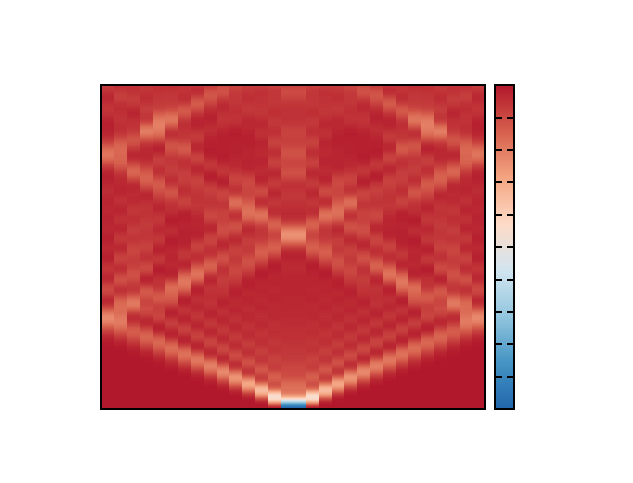
\includegraphics{Sz2_l0_mu0_2}}%
    \gplfronttext
  \end{picture}%
\endgroup
}
        \caption{$\mu=0.2$}
        \label{fig:testdouble3}
    \end{subfigure}
    \begin{subfigure}{.5\textwidth}
        \centering
        \resizebox{\textwidth}{!}{% GNUPLOT: LaTeX picture with Postscript
\begingroup
  \makeatletter
  \providecommand\color[2][]{%
    \GenericError{(gnuplot) \space\space\space\@spaces}{%
      Package color not loaded in conjunction with
      terminal option `colourtext'%
    }{See the gnuplot documentation for explanation.%
    }{Either use 'blacktext' in gnuplot or load the package
      color.sty in LaTeX.}%
    \renewcommand\color[2][]{}%
  }%
  \providecommand\includegraphics[2][]{%
    \GenericError{(gnuplot) \space\space\space\@spaces}{%
      Package graphicx or graphics not loaded%
    }{See the gnuplot documentation for explanation.%
    }{The gnuplot epslatex terminal needs graphicx.sty or graphics.sty.}%
    \renewcommand\includegraphics[2][]{}%
  }%
  \providecommand\rotatebox[2]{#2}%
  \@ifundefined{ifGPcolor}{%
    \newif\ifGPcolor
    \GPcolortrue
  }{}%
  \@ifundefined{ifGPblacktext}{%
    \newif\ifGPblacktext
    \GPblacktexttrue
  }{}%
  % define a \g@addto@macro without @ in the name:
  \let\gplgaddtomacro\g@addto@macro
  % define empty templates for all commands taking text:
  \gdef\gplbacktext{}%
  \gdef\gplfronttext{}%
  \makeatother
  \ifGPblacktext
    % no textcolor at all
    \def\colorrgb#1{}%
    \def\colorgray#1{}%
  \else
    % gray or color?
    \ifGPcolor
      \def\colorrgb#1{\color[rgb]{#1}}%
      \def\colorgray#1{\color[gray]{#1}}%
      \expandafter\def\csname LTw\endcsname{\color{white}}%
      \expandafter\def\csname LTb\endcsname{\color{black}}%
      \expandafter\def\csname LTa\endcsname{\color{black}}%
      \expandafter\def\csname LT0\endcsname{\color[rgb]{1,0,0}}%
      \expandafter\def\csname LT1\endcsname{\color[rgb]{0,1,0}}%
      \expandafter\def\csname LT2\endcsname{\color[rgb]{0,0,1}}%
      \expandafter\def\csname LT3\endcsname{\color[rgb]{1,0,1}}%
      \expandafter\def\csname LT4\endcsname{\color[rgb]{0,1,1}}%
      \expandafter\def\csname LT5\endcsname{\color[rgb]{1,1,0}}%
      \expandafter\def\csname LT6\endcsname{\color[rgb]{0,0,0}}%
      \expandafter\def\csname LT7\endcsname{\color[rgb]{1,0.3,0}}%
      \expandafter\def\csname LT8\endcsname{\color[rgb]{0.5,0.5,0.5}}%
    \else
      % gray
      \def\colorrgb#1{\color{black}}%
      \def\colorgray#1{\color[gray]{#1}}%
      \expandafter\def\csname LTw\endcsname{\color{white}}%
      \expandafter\def\csname LTb\endcsname{\color{black}}%
      \expandafter\def\csname LTa\endcsname{\color{black}}%
      \expandafter\def\csname LT0\endcsname{\color{black}}%
      \expandafter\def\csname LT1\endcsname{\color{black}}%
      \expandafter\def\csname LT2\endcsname{\color{black}}%
      \expandafter\def\csname LT3\endcsname{\color{black}}%
      \expandafter\def\csname LT4\endcsname{\color{black}}%
      \expandafter\def\csname LT5\endcsname{\color{black}}%
      \expandafter\def\csname LT6\endcsname{\color{black}}%
      \expandafter\def\csname LT7\endcsname{\color{black}}%
      \expandafter\def\csname LT8\endcsname{\color{black}}%
    \fi
  \fi
    \setlength{\unitlength}{0.0500bp}%
    \ifx\gptboxheight\undefined%
      \newlength{\gptboxheight}%
      \newlength{\gptboxwidth}%
      \newsavebox{\gptboxtext}%
    \fi%
    \setlength{\fboxrule}{0.5pt}%
    \setlength{\fboxsep}{1pt}%
\begin{picture}(5760.00,4320.00)%
    \gplgaddtomacro\gplbacktext{%
      \csname LTb\endcsname%
      \put(682,551){\makebox(0,0)[r]{\strut{}$0$}}%
      \put(682,1069){\makebox(0,0)[r]{\strut{}$10$}}%
      \put(682,1587){\makebox(0,0)[r]{\strut{}$20$}}%
      \put(682,2105){\makebox(0,0)[r]{\strut{}$30$}}%
      \put(682,2622){\makebox(0,0)[r]{\strut{}$40$}}%
      \put(682,3140){\makebox(0,0)[r]{\strut{}$50$}}%
      \put(682,3658){\makebox(0,0)[r]{\strut{}$60$}}%
      \put(875,330){\makebox(0,0){\strut{}$0$}}%
      \put(1489,330){\makebox(0,0){\strut{}$5$}}%
      \put(2103,330){\makebox(0,0){\strut{}$10$}}%
      \put(2717,330){\makebox(0,0){\strut{}$15$}}%
      \put(3331,330){\makebox(0,0){\strut{}$20$}}%
      \put(3945,330){\makebox(0,0){\strut{}$25$}}%
    }%
    \gplgaddtomacro\gplfronttext{%
      \csname LTb\endcsname%
      \put(176,2104){\rotatebox{-270}{\makebox(0,0){\strut{}time $t$}}}%
      \put(2656,0){\makebox(0,0){\strut{}particle index $i$}}%
      \put(2656,3989){\makebox(0,0){\strut{}$\lambda=0,~\mu=$0.3,~$N=30$}}%
      \csname LTb\endcsname%
      \put(4906,550){\makebox(0,0)[l]{\strut{}$-0.5$}}%
      \put(4906,860){\makebox(0,0)[l]{\strut{}$-0.4$}}%
      \put(4906,1171){\makebox(0,0)[l]{\strut{}$-0.3$}}%
      \put(4906,1482){\makebox(0,0)[l]{\strut{}$-0.2$}}%
      \put(4906,1793){\makebox(0,0)[l]{\strut{}$-0.1$}}%
      \put(4906,2104){\makebox(0,0)[l]{\strut{}$0$}}%
      \put(4906,2415){\makebox(0,0)[l]{\strut{}$0.1$}}%
      \put(4906,2726){\makebox(0,0)[l]{\strut{}$0.2$}}%
      \put(4906,3037){\makebox(0,0)[l]{\strut{}$0.3$}}%
      \put(4906,3348){\makebox(0,0)[l]{\strut{}$0.4$}}%
      \put(4906,3659){\makebox(0,0)[l]{\strut{}$0.5$}}%
      \put(5500,2104){\rotatebox{-270}{\makebox(0,0){\strut{}$\braket{S_1^z}_t$}}}%
    }%
    \gplbacktext
    \put(0,0){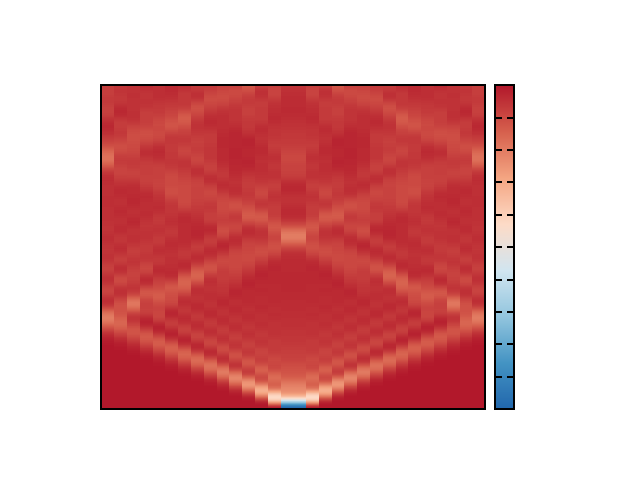
\includegraphics{Sz2_l0_mu0_3}}%
    \gplfronttext
  \end{picture}%
\endgroup
}
        \caption{$\mu=0.3$}
        \label{fig:testdouble4}
    \end{subfigure}
    \begin{subfigure}{.5\textwidth}
        \centering
        \resizebox{\textwidth}{!}{% GNUPLOT: LaTeX picture with Postscript
\begingroup
  \makeatletter
  \providecommand\color[2][]{%
    \GenericError{(gnuplot) \space\space\space\@spaces}{%
      Package color not loaded in conjunction with
      terminal option `colourtext'%
    }{See the gnuplot documentation for explanation.%
    }{Either use 'blacktext' in gnuplot or load the package
      color.sty in LaTeX.}%
    \renewcommand\color[2][]{}%
  }%
  \providecommand\includegraphics[2][]{%
    \GenericError{(gnuplot) \space\space\space\@spaces}{%
      Package graphicx or graphics not loaded%
    }{See the gnuplot documentation for explanation.%
    }{The gnuplot epslatex terminal needs graphicx.sty or graphics.sty.}%
    \renewcommand\includegraphics[2][]{}%
  }%
  \providecommand\rotatebox[2]{#2}%
  \@ifundefined{ifGPcolor}{%
    \newif\ifGPcolor
    \GPcolortrue
  }{}%
  \@ifundefined{ifGPblacktext}{%
    \newif\ifGPblacktext
    \GPblacktexttrue
  }{}%
  % define a \g@addto@macro without @ in the name:
  \let\gplgaddtomacro\g@addto@macro
  % define empty templates for all commands taking text:
  \gdef\gplbacktext{}%
  \gdef\gplfronttext{}%
  \makeatother
  \ifGPblacktext
    % no textcolor at all
    \def\colorrgb#1{}%
    \def\colorgray#1{}%
  \else
    % gray or color?
    \ifGPcolor
      \def\colorrgb#1{\color[rgb]{#1}}%
      \def\colorgray#1{\color[gray]{#1}}%
      \expandafter\def\csname LTw\endcsname{\color{white}}%
      \expandafter\def\csname LTb\endcsname{\color{black}}%
      \expandafter\def\csname LTa\endcsname{\color{black}}%
      \expandafter\def\csname LT0\endcsname{\color[rgb]{1,0,0}}%
      \expandafter\def\csname LT1\endcsname{\color[rgb]{0,1,0}}%
      \expandafter\def\csname LT2\endcsname{\color[rgb]{0,0,1}}%
      \expandafter\def\csname LT3\endcsname{\color[rgb]{1,0,1}}%
      \expandafter\def\csname LT4\endcsname{\color[rgb]{0,1,1}}%
      \expandafter\def\csname LT5\endcsname{\color[rgb]{1,1,0}}%
      \expandafter\def\csname LT6\endcsname{\color[rgb]{0,0,0}}%
      \expandafter\def\csname LT7\endcsname{\color[rgb]{1,0.3,0}}%
      \expandafter\def\csname LT8\endcsname{\color[rgb]{0.5,0.5,0.5}}%
    \else
      % gray
      \def\colorrgb#1{\color{black}}%
      \def\colorgray#1{\color[gray]{#1}}%
      \expandafter\def\csname LTw\endcsname{\color{white}}%
      \expandafter\def\csname LTb\endcsname{\color{black}}%
      \expandafter\def\csname LTa\endcsname{\color{black}}%
      \expandafter\def\csname LT0\endcsname{\color{black}}%
      \expandafter\def\csname LT1\endcsname{\color{black}}%
      \expandafter\def\csname LT2\endcsname{\color{black}}%
      \expandafter\def\csname LT3\endcsname{\color{black}}%
      \expandafter\def\csname LT4\endcsname{\color{black}}%
      \expandafter\def\csname LT5\endcsname{\color{black}}%
      \expandafter\def\csname LT6\endcsname{\color{black}}%
      \expandafter\def\csname LT7\endcsname{\color{black}}%
      \expandafter\def\csname LT8\endcsname{\color{black}}%
    \fi
  \fi
    \setlength{\unitlength}{0.0500bp}%
    \ifx\gptboxheight\undefined%
      \newlength{\gptboxheight}%
      \newlength{\gptboxwidth}%
      \newsavebox{\gptboxtext}%
    \fi%
    \setlength{\fboxrule}{0.5pt}%
    \setlength{\fboxsep}{1pt}%
\begin{picture}(5760.00,4320.00)%
    \gplgaddtomacro\gplbacktext{%
      \csname LTb\endcsname%
      \put(682,551){\makebox(0,0)[r]{\strut{}$0$}}%
      \put(682,1069){\makebox(0,0)[r]{\strut{}$10$}}%
      \put(682,1587){\makebox(0,0)[r]{\strut{}$20$}}%
      \put(682,2105){\makebox(0,0)[r]{\strut{}$30$}}%
      \put(682,2622){\makebox(0,0)[r]{\strut{}$40$}}%
      \put(682,3140){\makebox(0,0)[r]{\strut{}$50$}}%
      \put(682,3658){\makebox(0,0)[r]{\strut{}$60$}}%
      \put(875,330){\makebox(0,0){\strut{}$0$}}%
      \put(1489,330){\makebox(0,0){\strut{}$5$}}%
      \put(2103,330){\makebox(0,0){\strut{}$10$}}%
      \put(2717,330){\makebox(0,0){\strut{}$15$}}%
      \put(3331,330){\makebox(0,0){\strut{}$20$}}%
      \put(3945,330){\makebox(0,0){\strut{}$25$}}%
    }%
    \gplgaddtomacro\gplfronttext{%
      \csname LTb\endcsname%
      \put(176,2104){\rotatebox{-270}{\makebox(0,0){\strut{}time $t$}}}%
      \put(2656,0){\makebox(0,0){\strut{}particle index $i$}}%
      \put(2656,3989){\makebox(0,0){\strut{}$\lambda=0,~\mu=$0.4,~$N=30$}}%
      \csname LTb\endcsname%
      \put(4906,550){\makebox(0,0)[l]{\strut{}$-0.5$}}%
      \put(4906,860){\makebox(0,0)[l]{\strut{}$-0.4$}}%
      \put(4906,1171){\makebox(0,0)[l]{\strut{}$-0.3$}}%
      \put(4906,1482){\makebox(0,0)[l]{\strut{}$-0.2$}}%
      \put(4906,1793){\makebox(0,0)[l]{\strut{}$-0.1$}}%
      \put(4906,2104){\makebox(0,0)[l]{\strut{}$0$}}%
      \put(4906,2415){\makebox(0,0)[l]{\strut{}$0.1$}}%
      \put(4906,2726){\makebox(0,0)[l]{\strut{}$0.2$}}%
      \put(4906,3037){\makebox(0,0)[l]{\strut{}$0.3$}}%
      \put(4906,3348){\makebox(0,0)[l]{\strut{}$0.4$}}%
      \put(4906,3659){\makebox(0,0)[l]{\strut{}$0.5$}}%
      \put(5500,2104){\rotatebox{-270}{\makebox(0,0){\strut{}$\braket{S_1^z}_t$}}}%
    }%
    \gplbacktext
    \put(0,0){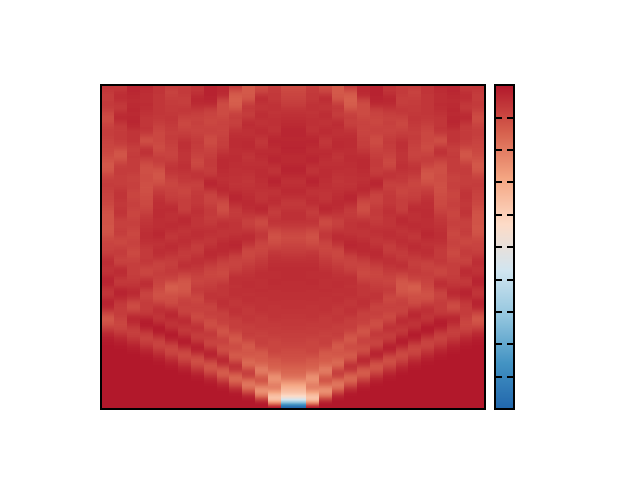
\includegraphics{Sz2_l0_mu0_4}}%
    \gplfronttext
  \end{picture}%
\endgroup
}
        \caption{$\mu=0.4$}
        \label{fig:testdouble5}
    \end{subfigure}
    \begin{subfigure}{.5\textwidth}
        \centering
        \resizebox{\textwidth}{!}{% GNUPLOT: LaTeX picture with Postscript
\begingroup
  \makeatletter
  \providecommand\color[2][]{%
    \GenericError{(gnuplot) \space\space\space\@spaces}{%
      Package color not loaded in conjunction with
      terminal option `colourtext'%
    }{See the gnuplot documentation for explanation.%
    }{Either use 'blacktext' in gnuplot or load the package
      color.sty in LaTeX.}%
    \renewcommand\color[2][]{}%
  }%
  \providecommand\includegraphics[2][]{%
    \GenericError{(gnuplot) \space\space\space\@spaces}{%
      Package graphicx or graphics not loaded%
    }{See the gnuplot documentation for explanation.%
    }{The gnuplot epslatex terminal needs graphicx.sty or graphics.sty.}%
    \renewcommand\includegraphics[2][]{}%
  }%
  \providecommand\rotatebox[2]{#2}%
  \@ifundefined{ifGPcolor}{%
    \newif\ifGPcolor
    \GPcolortrue
  }{}%
  \@ifundefined{ifGPblacktext}{%
    \newif\ifGPblacktext
    \GPblacktexttrue
  }{}%
  % define a \g@addto@macro without @ in the name:
  \let\gplgaddtomacro\g@addto@macro
  % define empty templates for all commands taking text:
  \gdef\gplbacktext{}%
  \gdef\gplfronttext{}%
  \makeatother
  \ifGPblacktext
    % no textcolor at all
    \def\colorrgb#1{}%
    \def\colorgray#1{}%
  \else
    % gray or color?
    \ifGPcolor
      \def\colorrgb#1{\color[rgb]{#1}}%
      \def\colorgray#1{\color[gray]{#1}}%
      \expandafter\def\csname LTw\endcsname{\color{white}}%
      \expandafter\def\csname LTb\endcsname{\color{black}}%
      \expandafter\def\csname LTa\endcsname{\color{black}}%
      \expandafter\def\csname LT0\endcsname{\color[rgb]{1,0,0}}%
      \expandafter\def\csname LT1\endcsname{\color[rgb]{0,1,0}}%
      \expandafter\def\csname LT2\endcsname{\color[rgb]{0,0,1}}%
      \expandafter\def\csname LT3\endcsname{\color[rgb]{1,0,1}}%
      \expandafter\def\csname LT4\endcsname{\color[rgb]{0,1,1}}%
      \expandafter\def\csname LT5\endcsname{\color[rgb]{1,1,0}}%
      \expandafter\def\csname LT6\endcsname{\color[rgb]{0,0,0}}%
      \expandafter\def\csname LT7\endcsname{\color[rgb]{1,0.3,0}}%
      \expandafter\def\csname LT8\endcsname{\color[rgb]{0.5,0.5,0.5}}%
    \else
      % gray
      \def\colorrgb#1{\color{black}}%
      \def\colorgray#1{\color[gray]{#1}}%
      \expandafter\def\csname LTw\endcsname{\color{white}}%
      \expandafter\def\csname LTb\endcsname{\color{black}}%
      \expandafter\def\csname LTa\endcsname{\color{black}}%
      \expandafter\def\csname LT0\endcsname{\color{black}}%
      \expandafter\def\csname LT1\endcsname{\color{black}}%
      \expandafter\def\csname LT2\endcsname{\color{black}}%
      \expandafter\def\csname LT3\endcsname{\color{black}}%
      \expandafter\def\csname LT4\endcsname{\color{black}}%
      \expandafter\def\csname LT5\endcsname{\color{black}}%
      \expandafter\def\csname LT6\endcsname{\color{black}}%
      \expandafter\def\csname LT7\endcsname{\color{black}}%
      \expandafter\def\csname LT8\endcsname{\color{black}}%
    \fi
  \fi
    \setlength{\unitlength}{0.0500bp}%
    \ifx\gptboxheight\undefined%
      \newlength{\gptboxheight}%
      \newlength{\gptboxwidth}%
      \newsavebox{\gptboxtext}%
    \fi%
    \setlength{\fboxrule}{0.5pt}%
    \setlength{\fboxsep}{1pt}%
\begin{picture}(5760.00,4320.00)%
    \gplgaddtomacro\gplbacktext{%
      \csname LTb\endcsname%
      \put(682,551){\makebox(0,0)[r]{\strut{}$0$}}%
      \put(682,1069){\makebox(0,0)[r]{\strut{}$10$}}%
      \put(682,1587){\makebox(0,0)[r]{\strut{}$20$}}%
      \put(682,2105){\makebox(0,0)[r]{\strut{}$30$}}%
      \put(682,2622){\makebox(0,0)[r]{\strut{}$40$}}%
      \put(682,3140){\makebox(0,0)[r]{\strut{}$50$}}%
      \put(682,3658){\makebox(0,0)[r]{\strut{}$60$}}%
      \put(875,330){\makebox(0,0){\strut{}$0$}}%
      \put(1489,330){\makebox(0,0){\strut{}$5$}}%
      \put(2103,330){\makebox(0,0){\strut{}$10$}}%
      \put(2717,330){\makebox(0,0){\strut{}$15$}}%
      \put(3331,330){\makebox(0,0){\strut{}$20$}}%
      \put(3945,330){\makebox(0,0){\strut{}$25$}}%
    }%
    \gplgaddtomacro\gplfronttext{%
      \csname LTb\endcsname%
      \put(176,2104){\rotatebox{-270}{\makebox(0,0){\strut{}time $Jt$}}}%
      \put(2656,0){\makebox(0,0){\strut{}particle index $i$}}%
      \put(2656,3989){\makebox(0,0){\strut{}$\lambda=0,~\mu=$0.5,~$N=30$}}%
      \csname LTb\endcsname%
      \put(4906,550){\makebox(0,0)[l]{\strut{}$-0.5$}}%
      \put(4906,860){\makebox(0,0)[l]{\strut{}$-0.4$}}%
      \put(4906,1171){\makebox(0,0)[l]{\strut{}$-0.3$}}%
      \put(4906,1482){\makebox(0,0)[l]{\strut{}$-0.2$}}%
      \put(4906,1793){\makebox(0,0)[l]{\strut{}$-0.1$}}%
      \put(4906,2104){\makebox(0,0)[l]{\strut{}$0$}}%
      \put(4906,2415){\makebox(0,0)[l]{\strut{}$0.1$}}%
      \put(4906,2726){\makebox(0,0)[l]{\strut{}$0.2$}}%
      \put(4906,3037){\makebox(0,0)[l]{\strut{}$0.3$}}%
      \put(4906,3348){\makebox(0,0)[l]{\strut{}$0.4$}}%
      \put(4906,3659){\makebox(0,0)[l]{\strut{}$0.5$}}%
      \put(5500,2104){\rotatebox{-270}{\makebox(0,0){\strut{}$\braket{S_1^z}_t$}}}%
    }%
    \gplbacktext
    \put(0,0){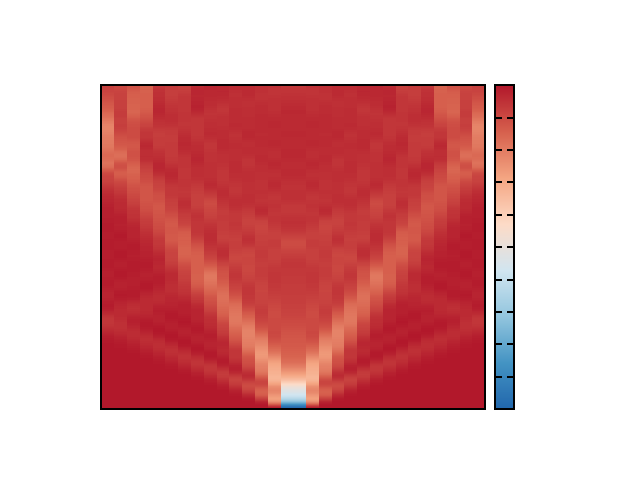
\includegraphics{Sz2_l0_mu0_5}}%
    \gplfronttext
  \end{picture}%
\endgroup
}
        \caption{$\mu=0.5$}
        \label{fig:testdouble6}
    \end{subfigure}
\end{figure}
\begin{figure}
    \ContinuedFloat
    \begin{subfigure}{.5\textwidth}
        \centering
        \resizebox{\textwidth}{!}{% GNUPLOT: LaTeX picture with Postscript
\begingroup
  \makeatletter
  \providecommand\color[2][]{%
    \GenericError{(gnuplot) \space\space\space\@spaces}{%
      Package color not loaded in conjunction with
      terminal option `colourtext'%
    }{See the gnuplot documentation for explanation.%
    }{Either use 'blacktext' in gnuplot or load the package
      color.sty in LaTeX.}%
    \renewcommand\color[2][]{}%
  }%
  \providecommand\includegraphics[2][]{%
    \GenericError{(gnuplot) \space\space\space\@spaces}{%
      Package graphicx or graphics not loaded%
    }{See the gnuplot documentation for explanation.%
    }{The gnuplot epslatex terminal needs graphicx.sty or graphics.sty.}%
    \renewcommand\includegraphics[2][]{}%
  }%
  \providecommand\rotatebox[2]{#2}%
  \@ifundefined{ifGPcolor}{%
    \newif\ifGPcolor
    \GPcolortrue
  }{}%
  \@ifundefined{ifGPblacktext}{%
    \newif\ifGPblacktext
    \GPblacktexttrue
  }{}%
  % define a \g@addto@macro without @ in the name:
  \let\gplgaddtomacro\g@addto@macro
  % define empty templates for all commands taking text:
  \gdef\gplbacktext{}%
  \gdef\gplfronttext{}%
  \makeatother
  \ifGPblacktext
    % no textcolor at all
    \def\colorrgb#1{}%
    \def\colorgray#1{}%
  \else
    % gray or color?
    \ifGPcolor
      \def\colorrgb#1{\color[rgb]{#1}}%
      \def\colorgray#1{\color[gray]{#1}}%
      \expandafter\def\csname LTw\endcsname{\color{white}}%
      \expandafter\def\csname LTb\endcsname{\color{black}}%
      \expandafter\def\csname LTa\endcsname{\color{black}}%
      \expandafter\def\csname LT0\endcsname{\color[rgb]{1,0,0}}%
      \expandafter\def\csname LT1\endcsname{\color[rgb]{0,1,0}}%
      \expandafter\def\csname LT2\endcsname{\color[rgb]{0,0,1}}%
      \expandafter\def\csname LT3\endcsname{\color[rgb]{1,0,1}}%
      \expandafter\def\csname LT4\endcsname{\color[rgb]{0,1,1}}%
      \expandafter\def\csname LT5\endcsname{\color[rgb]{1,1,0}}%
      \expandafter\def\csname LT6\endcsname{\color[rgb]{0,0,0}}%
      \expandafter\def\csname LT7\endcsname{\color[rgb]{1,0.3,0}}%
      \expandafter\def\csname LT8\endcsname{\color[rgb]{0.5,0.5,0.5}}%
    \else
      % gray
      \def\colorrgb#1{\color{black}}%
      \def\colorgray#1{\color[gray]{#1}}%
      \expandafter\def\csname LTw\endcsname{\color{white}}%
      \expandafter\def\csname LTb\endcsname{\color{black}}%
      \expandafter\def\csname LTa\endcsname{\color{black}}%
      \expandafter\def\csname LT0\endcsname{\color{black}}%
      \expandafter\def\csname LT1\endcsname{\color{black}}%
      \expandafter\def\csname LT2\endcsname{\color{black}}%
      \expandafter\def\csname LT3\endcsname{\color{black}}%
      \expandafter\def\csname LT4\endcsname{\color{black}}%
      \expandafter\def\csname LT5\endcsname{\color{black}}%
      \expandafter\def\csname LT6\endcsname{\color{black}}%
      \expandafter\def\csname LT7\endcsname{\color{black}}%
      \expandafter\def\csname LT8\endcsname{\color{black}}%
    \fi
  \fi
    \setlength{\unitlength}{0.0500bp}%
    \ifx\gptboxheight\undefined%
      \newlength{\gptboxheight}%
      \newlength{\gptboxwidth}%
      \newsavebox{\gptboxtext}%
    \fi%
    \setlength{\fboxrule}{0.5pt}%
    \setlength{\fboxsep}{1pt}%
\begin{picture}(5760.00,4320.00)%
    \gplgaddtomacro\gplbacktext{%
      \csname LTb\endcsname%
      \put(682,551){\makebox(0,0)[r]{\strut{}$0$}}%
      \put(682,1069){\makebox(0,0)[r]{\strut{}$10$}}%
      \put(682,1587){\makebox(0,0)[r]{\strut{}$20$}}%
      \put(682,2105){\makebox(0,0)[r]{\strut{}$30$}}%
      \put(682,2622){\makebox(0,0)[r]{\strut{}$40$}}%
      \put(682,3140){\makebox(0,0)[r]{\strut{}$50$}}%
      \put(682,3658){\makebox(0,0)[r]{\strut{}$60$}}%
      \put(875,330){\makebox(0,0){\strut{}$0$}}%
      \put(1489,330){\makebox(0,0){\strut{}$5$}}%
      \put(2103,330){\makebox(0,0){\strut{}$10$}}%
      \put(2717,330){\makebox(0,0){\strut{}$15$}}%
      \put(3331,330){\makebox(0,0){\strut{}$20$}}%
      \put(3945,330){\makebox(0,0){\strut{}$25$}}%
    }%
    \gplgaddtomacro\gplfronttext{%
      \csname LTb\endcsname%
      \put(176,2104){\rotatebox{-270}{\makebox(0,0){\strut{}time $t$}}}%
      \put(2656,0){\makebox(0,0){\strut{}particle index $i$}}%
      \put(2656,3989){\makebox(0,0){\strut{}$\lambda=0,~\mu=$0.6,~$N=30$}}%
      \csname LTb\endcsname%
      \put(4906,550){\makebox(0,0)[l]{\strut{}$-0.5$}}%
      \put(4906,860){\makebox(0,0)[l]{\strut{}$-0.4$}}%
      \put(4906,1171){\makebox(0,0)[l]{\strut{}$-0.3$}}%
      \put(4906,1482){\makebox(0,0)[l]{\strut{}$-0.2$}}%
      \put(4906,1793){\makebox(0,0)[l]{\strut{}$-0.1$}}%
      \put(4906,2104){\makebox(0,0)[l]{\strut{}$0$}}%
      \put(4906,2415){\makebox(0,0)[l]{\strut{}$0.1$}}%
      \put(4906,2726){\makebox(0,0)[l]{\strut{}$0.2$}}%
      \put(4906,3037){\makebox(0,0)[l]{\strut{}$0.3$}}%
      \put(4906,3348){\makebox(0,0)[l]{\strut{}$0.4$}}%
      \put(4906,3659){\makebox(0,0)[l]{\strut{}$0.5$}}%
      \put(5500,2104){\rotatebox{-270}{\makebox(0,0){\strut{}$\braket{S_1^z}_t$}}}%
    }%
    \gplbacktext
    \put(0,0){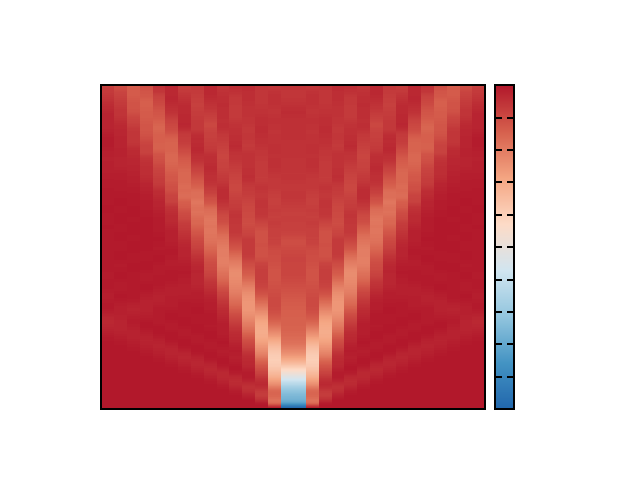
\includegraphics{Sz2_l0_mu0_6}}%
    \gplfronttext
  \end{picture}%
\endgroup
}
        \caption{$\mu=0.6$}
        \label{fig:testdouble7}
    \end{subfigure}
    \begin{subfigure}{.5\textwidth}
        \centering
        \resizebox{\textwidth}{!}{% GNUPLOT: LaTeX picture with Postscript
\begingroup
  \makeatletter
  \providecommand\color[2][]{%
    \GenericError{(gnuplot) \space\space\space\@spaces}{%
      Package color not loaded in conjunction with
      terminal option `colourtext'%
    }{See the gnuplot documentation for explanation.%
    }{Either use 'blacktext' in gnuplot or load the package
      color.sty in LaTeX.}%
    \renewcommand\color[2][]{}%
  }%
  \providecommand\includegraphics[2][]{%
    \GenericError{(gnuplot) \space\space\space\@spaces}{%
      Package graphicx or graphics not loaded%
    }{See the gnuplot documentation for explanation.%
    }{The gnuplot epslatex terminal needs graphicx.sty or graphics.sty.}%
    \renewcommand\includegraphics[2][]{}%
  }%
  \providecommand\rotatebox[2]{#2}%
  \@ifundefined{ifGPcolor}{%
    \newif\ifGPcolor
    \GPcolortrue
  }{}%
  \@ifundefined{ifGPblacktext}{%
    \newif\ifGPblacktext
    \GPblacktexttrue
  }{}%
  % define a \g@addto@macro without @ in the name:
  \let\gplgaddtomacro\g@addto@macro
  % define empty templates for all commands taking text:
  \gdef\gplbacktext{}%
  \gdef\gplfronttext{}%
  \makeatother
  \ifGPblacktext
    % no textcolor at all
    \def\colorrgb#1{}%
    \def\colorgray#1{}%
  \else
    % gray or color?
    \ifGPcolor
      \def\colorrgb#1{\color[rgb]{#1}}%
      \def\colorgray#1{\color[gray]{#1}}%
      \expandafter\def\csname LTw\endcsname{\color{white}}%
      \expandafter\def\csname LTb\endcsname{\color{black}}%
      \expandafter\def\csname LTa\endcsname{\color{black}}%
      \expandafter\def\csname LT0\endcsname{\color[rgb]{1,0,0}}%
      \expandafter\def\csname LT1\endcsname{\color[rgb]{0,1,0}}%
      \expandafter\def\csname LT2\endcsname{\color[rgb]{0,0,1}}%
      \expandafter\def\csname LT3\endcsname{\color[rgb]{1,0,1}}%
      \expandafter\def\csname LT4\endcsname{\color[rgb]{0,1,1}}%
      \expandafter\def\csname LT5\endcsname{\color[rgb]{1,1,0}}%
      \expandafter\def\csname LT6\endcsname{\color[rgb]{0,0,0}}%
      \expandafter\def\csname LT7\endcsname{\color[rgb]{1,0.3,0}}%
      \expandafter\def\csname LT8\endcsname{\color[rgb]{0.5,0.5,0.5}}%
    \else
      % gray
      \def\colorrgb#1{\color{black}}%
      \def\colorgray#1{\color[gray]{#1}}%
      \expandafter\def\csname LTw\endcsname{\color{white}}%
      \expandafter\def\csname LTb\endcsname{\color{black}}%
      \expandafter\def\csname LTa\endcsname{\color{black}}%
      \expandafter\def\csname LT0\endcsname{\color{black}}%
      \expandafter\def\csname LT1\endcsname{\color{black}}%
      \expandafter\def\csname LT2\endcsname{\color{black}}%
      \expandafter\def\csname LT3\endcsname{\color{black}}%
      \expandafter\def\csname LT4\endcsname{\color{black}}%
      \expandafter\def\csname LT5\endcsname{\color{black}}%
      \expandafter\def\csname LT6\endcsname{\color{black}}%
      \expandafter\def\csname LT7\endcsname{\color{black}}%
      \expandafter\def\csname LT8\endcsname{\color{black}}%
    \fi
  \fi
    \setlength{\unitlength}{0.0500bp}%
    \ifx\gptboxheight\undefined%
      \newlength{\gptboxheight}%
      \newlength{\gptboxwidth}%
      \newsavebox{\gptboxtext}%
    \fi%
    \setlength{\fboxrule}{0.5pt}%
    \setlength{\fboxsep}{1pt}%
\begin{picture}(5760.00,4320.00)%
    \gplgaddtomacro\gplbacktext{%
      \csname LTb\endcsname%
      \put(682,551){\makebox(0,0)[r]{\strut{}$0$}}%
      \put(682,1069){\makebox(0,0)[r]{\strut{}$10$}}%
      \put(682,1587){\makebox(0,0)[r]{\strut{}$20$}}%
      \put(682,2105){\makebox(0,0)[r]{\strut{}$30$}}%
      \put(682,2622){\makebox(0,0)[r]{\strut{}$40$}}%
      \put(682,3140){\makebox(0,0)[r]{\strut{}$50$}}%
      \put(682,3658){\makebox(0,0)[r]{\strut{}$60$}}%
      \put(875,330){\makebox(0,0){\strut{}$0$}}%
      \put(1489,330){\makebox(0,0){\strut{}$5$}}%
      \put(2103,330){\makebox(0,0){\strut{}$10$}}%
      \put(2717,330){\makebox(0,0){\strut{}$15$}}%
      \put(3331,330){\makebox(0,0){\strut{}$20$}}%
      \put(3945,330){\makebox(0,0){\strut{}$25$}}%
    }%
    \gplgaddtomacro\gplfronttext{%
      \csname LTb\endcsname%
      \put(176,2104){\rotatebox{-270}{\makebox(0,0){\strut{}time $Jt$}}}%
      \put(2656,0){\makebox(0,0){\strut{}particle index $i$}}%
      \put(2656,3989){\makebox(0,0){\strut{}$\lambda=0,~\mu=$0.7,~$N=30$}}%
      \csname LTb\endcsname%
      \put(4906,550){\makebox(0,0)[l]{\strut{}$-0.5$}}%
      \put(4906,860){\makebox(0,0)[l]{\strut{}$-0.4$}}%
      \put(4906,1171){\makebox(0,0)[l]{\strut{}$-0.3$}}%
      \put(4906,1482){\makebox(0,0)[l]{\strut{}$-0.2$}}%
      \put(4906,1793){\makebox(0,0)[l]{\strut{}$-0.1$}}%
      \put(4906,2104){\makebox(0,0)[l]{\strut{}$0$}}%
      \put(4906,2415){\makebox(0,0)[l]{\strut{}$0.1$}}%
      \put(4906,2726){\makebox(0,0)[l]{\strut{}$0.2$}}%
      \put(4906,3037){\makebox(0,0)[l]{\strut{}$0.3$}}%
      \put(4906,3348){\makebox(0,0)[l]{\strut{}$0.4$}}%
      \put(4906,3659){\makebox(0,0)[l]{\strut{}$0.5$}}%
      \put(5500,2104){\rotatebox{-270}{\makebox(0,0){\strut{}$\braket{S_1^z}_t$}}}%
    }%
    \gplbacktext
    \put(0,0){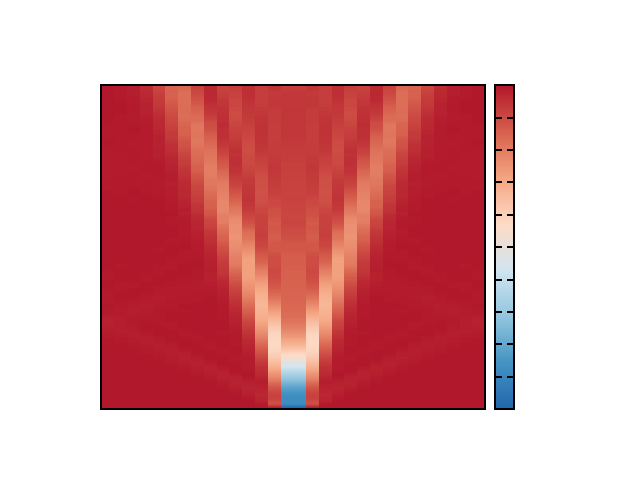
\includegraphics{Sz2_l0_mu0_7}}%
    \gplfronttext
  \end{picture}%
\endgroup
}
        \caption{$\mu=0.7$}
        \label{fig:testdouble8}
    \end{subfigure}
    \begin{subfigure}{.5\textwidth}
        \centering
        \resizebox{\textwidth}{!}{% GNUPLOT: LaTeX picture with Postscript
\begingroup
  \makeatletter
  \providecommand\color[2][]{%
    \GenericError{(gnuplot) \space\space\space\@spaces}{%
      Package color not loaded in conjunction with
      terminal option `colourtext'%
    }{See the gnuplot documentation for explanation.%
    }{Either use 'blacktext' in gnuplot or load the package
      color.sty in LaTeX.}%
    \renewcommand\color[2][]{}%
  }%
  \providecommand\includegraphics[2][]{%
    \GenericError{(gnuplot) \space\space\space\@spaces}{%
      Package graphicx or graphics not loaded%
    }{See the gnuplot documentation for explanation.%
    }{The gnuplot epslatex terminal needs graphicx.sty or graphics.sty.}%
    \renewcommand\includegraphics[2][]{}%
  }%
  \providecommand\rotatebox[2]{#2}%
  \@ifundefined{ifGPcolor}{%
    \newif\ifGPcolor
    \GPcolortrue
  }{}%
  \@ifundefined{ifGPblacktext}{%
    \newif\ifGPblacktext
    \GPblacktexttrue
  }{}%
  % define a \g@addto@macro without @ in the name:
  \let\gplgaddtomacro\g@addto@macro
  % define empty templates for all commands taking text:
  \gdef\gplbacktext{}%
  \gdef\gplfronttext{}%
  \makeatother
  \ifGPblacktext
    % no textcolor at all
    \def\colorrgb#1{}%
    \def\colorgray#1{}%
  \else
    % gray or color?
    \ifGPcolor
      \def\colorrgb#1{\color[rgb]{#1}}%
      \def\colorgray#1{\color[gray]{#1}}%
      \expandafter\def\csname LTw\endcsname{\color{white}}%
      \expandafter\def\csname LTb\endcsname{\color{black}}%
      \expandafter\def\csname LTa\endcsname{\color{black}}%
      \expandafter\def\csname LT0\endcsname{\color[rgb]{1,0,0}}%
      \expandafter\def\csname LT1\endcsname{\color[rgb]{0,1,0}}%
      \expandafter\def\csname LT2\endcsname{\color[rgb]{0,0,1}}%
      \expandafter\def\csname LT3\endcsname{\color[rgb]{1,0,1}}%
      \expandafter\def\csname LT4\endcsname{\color[rgb]{0,1,1}}%
      \expandafter\def\csname LT5\endcsname{\color[rgb]{1,1,0}}%
      \expandafter\def\csname LT6\endcsname{\color[rgb]{0,0,0}}%
      \expandafter\def\csname LT7\endcsname{\color[rgb]{1,0.3,0}}%
      \expandafter\def\csname LT8\endcsname{\color[rgb]{0.5,0.5,0.5}}%
    \else
      % gray
      \def\colorrgb#1{\color{black}}%
      \def\colorgray#1{\color[gray]{#1}}%
      \expandafter\def\csname LTw\endcsname{\color{white}}%
      \expandafter\def\csname LTb\endcsname{\color{black}}%
      \expandafter\def\csname LTa\endcsname{\color{black}}%
      \expandafter\def\csname LT0\endcsname{\color{black}}%
      \expandafter\def\csname LT1\endcsname{\color{black}}%
      \expandafter\def\csname LT2\endcsname{\color{black}}%
      \expandafter\def\csname LT3\endcsname{\color{black}}%
      \expandafter\def\csname LT4\endcsname{\color{black}}%
      \expandafter\def\csname LT5\endcsname{\color{black}}%
      \expandafter\def\csname LT6\endcsname{\color{black}}%
      \expandafter\def\csname LT7\endcsname{\color{black}}%
      \expandafter\def\csname LT8\endcsname{\color{black}}%
    \fi
  \fi
    \setlength{\unitlength}{0.0500bp}%
    \ifx\gptboxheight\undefined%
      \newlength{\gptboxheight}%
      \newlength{\gptboxwidth}%
      \newsavebox{\gptboxtext}%
    \fi%
    \setlength{\fboxrule}{0.5pt}%
    \setlength{\fboxsep}{1pt}%
\begin{picture}(5760.00,4320.00)%
    \gplgaddtomacro\gplbacktext{%
      \csname LTb\endcsname%
      \put(682,551){\makebox(0,0)[r]{\strut{}$0$}}%
      \put(682,1069){\makebox(0,0)[r]{\strut{}$10$}}%
      \put(682,1587){\makebox(0,0)[r]{\strut{}$20$}}%
      \put(682,2105){\makebox(0,0)[r]{\strut{}$30$}}%
      \put(682,2622){\makebox(0,0)[r]{\strut{}$40$}}%
      \put(682,3140){\makebox(0,0)[r]{\strut{}$50$}}%
      \put(682,3658){\makebox(0,0)[r]{\strut{}$60$}}%
      \put(875,330){\makebox(0,0){\strut{}$0$}}%
      \put(1489,330){\makebox(0,0){\strut{}$5$}}%
      \put(2103,330){\makebox(0,0){\strut{}$10$}}%
      \put(2717,330){\makebox(0,0){\strut{}$15$}}%
      \put(3331,330){\makebox(0,0){\strut{}$20$}}%
      \put(3945,330){\makebox(0,0){\strut{}$25$}}%
    }%
    \gplgaddtomacro\gplfronttext{%
      \csname LTb\endcsname%
      \put(176,2104){\rotatebox{-270}{\makebox(0,0){\strut{}time $t$}}}%
      \put(2656,0){\makebox(0,0){\strut{}particle index $i$}}%
      \put(2656,3989){\makebox(0,0){\strut{}$\lambda=0,~\mu=$0.8,~$N=30$}}%
      \csname LTb\endcsname%
      \put(4906,550){\makebox(0,0)[l]{\strut{}$-0.5$}}%
      \put(4906,860){\makebox(0,0)[l]{\strut{}$-0.4$}}%
      \put(4906,1171){\makebox(0,0)[l]{\strut{}$-0.3$}}%
      \put(4906,1482){\makebox(0,0)[l]{\strut{}$-0.2$}}%
      \put(4906,1793){\makebox(0,0)[l]{\strut{}$-0.1$}}%
      \put(4906,2104){\makebox(0,0)[l]{\strut{}$0$}}%
      \put(4906,2415){\makebox(0,0)[l]{\strut{}$0.1$}}%
      \put(4906,2726){\makebox(0,0)[l]{\strut{}$0.2$}}%
      \put(4906,3037){\makebox(0,0)[l]{\strut{}$0.3$}}%
      \put(4906,3348){\makebox(0,0)[l]{\strut{}$0.4$}}%
      \put(4906,3659){\makebox(0,0)[l]{\strut{}$0.5$}}%
      \put(5500,2104){\rotatebox{-270}{\makebox(0,0){\strut{}$\braket{S_1^z}_t$}}}%
    }%
    \gplbacktext
    \put(0,0){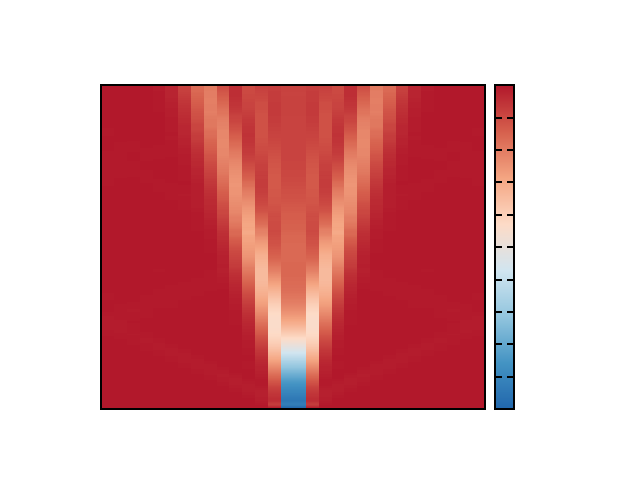
\includegraphics{Sz2_l0_mu0_8}}%
    \gplfronttext
  \end{picture}%
\endgroup
}
        \caption{$\mu=0.8$}
        \label{fig:testdouble9}
    \end{subfigure}
    \begin{subfigure}{.5\textwidth}
        \centering
        \resizebox{\textwidth}{!}{% GNUPLOT: LaTeX picture with Postscript
\begingroup
  \makeatletter
  \providecommand\color[2][]{%
    \GenericError{(gnuplot) \space\space\space\@spaces}{%
      Package color not loaded in conjunction with
      terminal option `colourtext'%
    }{See the gnuplot documentation for explanation.%
    }{Either use 'blacktext' in gnuplot or load the package
      color.sty in LaTeX.}%
    \renewcommand\color[2][]{}%
  }%
  \providecommand\includegraphics[2][]{%
    \GenericError{(gnuplot) \space\space\space\@spaces}{%
      Package graphicx or graphics not loaded%
    }{See the gnuplot documentation for explanation.%
    }{The gnuplot epslatex terminal needs graphicx.sty or graphics.sty.}%
    \renewcommand\includegraphics[2][]{}%
  }%
  \providecommand\rotatebox[2]{#2}%
  \@ifundefined{ifGPcolor}{%
    \newif\ifGPcolor
    \GPcolortrue
  }{}%
  \@ifundefined{ifGPblacktext}{%
    \newif\ifGPblacktext
    \GPblacktexttrue
  }{}%
  % define a \g@addto@macro without @ in the name:
  \let\gplgaddtomacro\g@addto@macro
  % define empty templates for all commands taking text:
  \gdef\gplbacktext{}%
  \gdef\gplfronttext{}%
  \makeatother
  \ifGPblacktext
    % no textcolor at all
    \def\colorrgb#1{}%
    \def\colorgray#1{}%
  \else
    % gray or color?
    \ifGPcolor
      \def\colorrgb#1{\color[rgb]{#1}}%
      \def\colorgray#1{\color[gray]{#1}}%
      \expandafter\def\csname LTw\endcsname{\color{white}}%
      \expandafter\def\csname LTb\endcsname{\color{black}}%
      \expandafter\def\csname LTa\endcsname{\color{black}}%
      \expandafter\def\csname LT0\endcsname{\color[rgb]{1,0,0}}%
      \expandafter\def\csname LT1\endcsname{\color[rgb]{0,1,0}}%
      \expandafter\def\csname LT2\endcsname{\color[rgb]{0,0,1}}%
      \expandafter\def\csname LT3\endcsname{\color[rgb]{1,0,1}}%
      \expandafter\def\csname LT4\endcsname{\color[rgb]{0,1,1}}%
      \expandafter\def\csname LT5\endcsname{\color[rgb]{1,1,0}}%
      \expandafter\def\csname LT6\endcsname{\color[rgb]{0,0,0}}%
      \expandafter\def\csname LT7\endcsname{\color[rgb]{1,0.3,0}}%
      \expandafter\def\csname LT8\endcsname{\color[rgb]{0.5,0.5,0.5}}%
    \else
      % gray
      \def\colorrgb#1{\color{black}}%
      \def\colorgray#1{\color[gray]{#1}}%
      \expandafter\def\csname LTw\endcsname{\color{white}}%
      \expandafter\def\csname LTb\endcsname{\color{black}}%
      \expandafter\def\csname LTa\endcsname{\color{black}}%
      \expandafter\def\csname LT0\endcsname{\color{black}}%
      \expandafter\def\csname LT1\endcsname{\color{black}}%
      \expandafter\def\csname LT2\endcsname{\color{black}}%
      \expandafter\def\csname LT3\endcsname{\color{black}}%
      \expandafter\def\csname LT4\endcsname{\color{black}}%
      \expandafter\def\csname LT5\endcsname{\color{black}}%
      \expandafter\def\csname LT6\endcsname{\color{black}}%
      \expandafter\def\csname LT7\endcsname{\color{black}}%
      \expandafter\def\csname LT8\endcsname{\color{black}}%
    \fi
  \fi
    \setlength{\unitlength}{0.0500bp}%
    \ifx\gptboxheight\undefined%
      \newlength{\gptboxheight}%
      \newlength{\gptboxwidth}%
      \newsavebox{\gptboxtext}%
    \fi%
    \setlength{\fboxrule}{0.5pt}%
    \setlength{\fboxsep}{1pt}%
\begin{picture}(5760.00,4320.00)%
    \gplgaddtomacro\gplbacktext{%
      \csname LTb\endcsname%
      \put(682,551){\makebox(0,0)[r]{\strut{}$0$}}%
      \put(682,1069){\makebox(0,0)[r]{\strut{}$10$}}%
      \put(682,1587){\makebox(0,0)[r]{\strut{}$20$}}%
      \put(682,2105){\makebox(0,0)[r]{\strut{}$30$}}%
      \put(682,2622){\makebox(0,0)[r]{\strut{}$40$}}%
      \put(682,3140){\makebox(0,0)[r]{\strut{}$50$}}%
      \put(682,3658){\makebox(0,0)[r]{\strut{}$60$}}%
      \put(875,330){\makebox(0,0){\strut{}$0$}}%
      \put(1489,330){\makebox(0,0){\strut{}$5$}}%
      \put(2103,330){\makebox(0,0){\strut{}$10$}}%
      \put(2717,330){\makebox(0,0){\strut{}$15$}}%
      \put(3331,330){\makebox(0,0){\strut{}$20$}}%
      \put(3945,330){\makebox(0,0){\strut{}$25$}}%
    }%
    \gplgaddtomacro\gplfronttext{%
      \csname LTb\endcsname%
      \put(176,2104){\rotatebox{-270}{\makebox(0,0){\strut{}time $Jt$}}}%
      \put(2656,0){\makebox(0,0){\strut{}particle index $i$}}%
      \put(2656,3989){\makebox(0,0){\strut{}$\lambda=0,~\mu=$0.9,~$N=30$}}%
      \csname LTb\endcsname%
      \put(4906,550){\makebox(0,0)[l]{\strut{}$-0.5$}}%
      \put(4906,860){\makebox(0,0)[l]{\strut{}$-0.4$}}%
      \put(4906,1171){\makebox(0,0)[l]{\strut{}$-0.3$}}%
      \put(4906,1482){\makebox(0,0)[l]{\strut{}$-0.2$}}%
      \put(4906,1793){\makebox(0,0)[l]{\strut{}$-0.1$}}%
      \put(4906,2104){\makebox(0,0)[l]{\strut{}$0$}}%
      \put(4906,2415){\makebox(0,0)[l]{\strut{}$0.1$}}%
      \put(4906,2726){\makebox(0,0)[l]{\strut{}$0.2$}}%
      \put(4906,3037){\makebox(0,0)[l]{\strut{}$0.3$}}%
      \put(4906,3348){\makebox(0,0)[l]{\strut{}$0.4$}}%
      \put(4906,3659){\makebox(0,0)[l]{\strut{}$0.5$}}%
      \put(5500,2104){\rotatebox{-270}{\makebox(0,0){\strut{}$\braket{S_1^z}_t$}}}%
    }%
    \gplbacktext
    \put(0,0){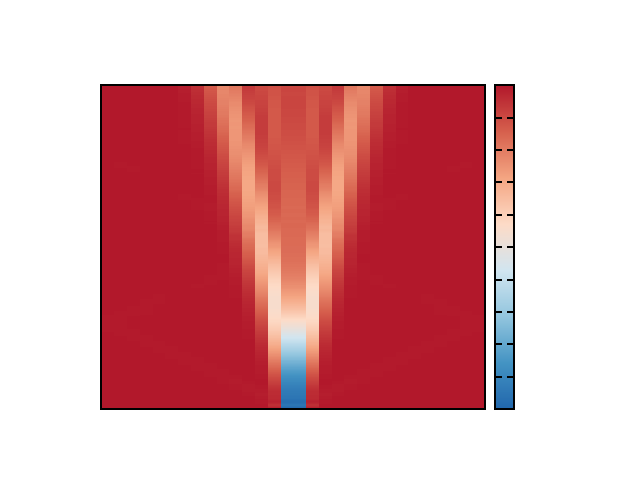
\includegraphics{Sz2_l0_mu0_9}}%
    \gplfronttext
  \end{picture}%
\endgroup
}
        \caption{$\mu=0.9$}
        \label{fig:testdouble10}
    \end{subfigure}
    \caption{Two string magnon propagation for $\lambda=0, N=30$ for varying $\mu$. For increasing $\mu$, slower propagation cascades coming from bound spins can be observed.}
\end{figure}
\subsection{Magnon scattering}
When two propagating magnons collide, it can be understood as a scattering event. As \cite{solitonscattering} outlines, this leads to a displacement. In \cref{fig:testcollision1,fig:testcollision2} a collision between a two-string magnon and a single magnon are shown. In \cref{fig:testcollision1} for $\mu=0$ no displacement can be observed. In \cref{fig:testcollision2} for $\mu=5$, there is a clear displacement of the single magnon as it collides with the other: The propagation cascade is shifted to the left, which is in analogy to \cite[fig.\,5]{solitonscattering}.
\begin{figure}
    \begin{subfigure}{.5\textwidth}
        \centering
        \resizebox{\textwidth}{!}{% GNUPLOT: LaTeX picture with Postscript
\begingroup
  \makeatletter
  \providecommand\color[2][]{%
    \GenericError{(gnuplot) \space\space\space\@spaces}{%
      Package color not loaded in conjunction with
      terminal option `colourtext'%
    }{See the gnuplot documentation for explanation.%
    }{Either use 'blacktext' in gnuplot or load the package
      color.sty in LaTeX.}%
    \renewcommand\color[2][]{}%
  }%
  \providecommand\includegraphics[2][]{%
    \GenericError{(gnuplot) \space\space\space\@spaces}{%
      Package graphicx or graphics not loaded%
    }{See the gnuplot documentation for explanation.%
    }{The gnuplot epslatex terminal needs graphicx.sty or graphics.sty.}%
    \renewcommand\includegraphics[2][]{}%
  }%
  \providecommand\rotatebox[2]{#2}%
  \@ifundefined{ifGPcolor}{%
    \newif\ifGPcolor
    \GPcolortrue
  }{}%
  \@ifundefined{ifGPblacktext}{%
    \newif\ifGPblacktext
    \GPblacktexttrue
  }{}%
  % define a \g@addto@macro without @ in the name:
  \let\gplgaddtomacro\g@addto@macro
  % define empty templates for all commands taking text:
  \gdef\gplbacktext{}%
  \gdef\gplfronttext{}%
  \makeatother
  \ifGPblacktext
    % no textcolor at all
    \def\colorrgb#1{}%
    \def\colorgray#1{}%
  \else
    % gray or color?
    \ifGPcolor
      \def\colorrgb#1{\color[rgb]{#1}}%
      \def\colorgray#1{\color[gray]{#1}}%
      \expandafter\def\csname LTw\endcsname{\color{white}}%
      \expandafter\def\csname LTb\endcsname{\color{black}}%
      \expandafter\def\csname LTa\endcsname{\color{black}}%
      \expandafter\def\csname LT0\endcsname{\color[rgb]{1,0,0}}%
      \expandafter\def\csname LT1\endcsname{\color[rgb]{0,1,0}}%
      \expandafter\def\csname LT2\endcsname{\color[rgb]{0,0,1}}%
      \expandafter\def\csname LT3\endcsname{\color[rgb]{1,0,1}}%
      \expandafter\def\csname LT4\endcsname{\color[rgb]{0,1,1}}%
      \expandafter\def\csname LT5\endcsname{\color[rgb]{1,1,0}}%
      \expandafter\def\csname LT6\endcsname{\color[rgb]{0,0,0}}%
      \expandafter\def\csname LT7\endcsname{\color[rgb]{1,0.3,0}}%
      \expandafter\def\csname LT8\endcsname{\color[rgb]{0.5,0.5,0.5}}%
    \else
      % gray
      \def\colorrgb#1{\color{black}}%
      \def\colorgray#1{\color[gray]{#1}}%
      \expandafter\def\csname LTw\endcsname{\color{white}}%
      \expandafter\def\csname LTb\endcsname{\color{black}}%
      \expandafter\def\csname LTa\endcsname{\color{black}}%
      \expandafter\def\csname LT0\endcsname{\color{black}}%
      \expandafter\def\csname LT1\endcsname{\color{black}}%
      \expandafter\def\csname LT2\endcsname{\color{black}}%
      \expandafter\def\csname LT3\endcsname{\color{black}}%
      \expandafter\def\csname LT4\endcsname{\color{black}}%
      \expandafter\def\csname LT5\endcsname{\color{black}}%
      \expandafter\def\csname LT6\endcsname{\color{black}}%
      \expandafter\def\csname LT7\endcsname{\color{black}}%
      \expandafter\def\csname LT8\endcsname{\color{black}}%
    \fi
  \fi
    \setlength{\unitlength}{0.0500bp}%
    \ifx\gptboxheight\undefined%
      \newlength{\gptboxheight}%
      \newlength{\gptboxwidth}%
      \newsavebox{\gptboxtext}%
    \fi%
    \setlength{\fboxrule}{0.5pt}%
    \setlength{\fboxsep}{1pt}%
\begin{picture}(5760.00,5760.00)%
    \gplgaddtomacro\gplbacktext{%
      \csname LTb\endcsname%
      \put(550,709){\makebox(0,0)[r]{\strut{}$0$}}%
      \put(550,1257){\makebox(0,0)[r]{\strut{}$1$}}%
      \put(550,1805){\makebox(0,0)[r]{\strut{}$2$}}%
      \put(550,2353){\makebox(0,0)[r]{\strut{}$3$}}%
      \put(550,2902){\makebox(0,0)[r]{\strut{}$4$}}%
      \put(550,3450){\makebox(0,0)[r]{\strut{}$5$}}%
      \put(550,3998){\makebox(0,0)[r]{\strut{}$6$}}%
      \put(550,4546){\makebox(0,0)[r]{\strut{}$7$}}%
      \put(550,5094){\makebox(0,0)[r]{\strut{}$8$}}%
      \put(761,484){\makebox(0,0){\strut{}$0$}}%
      \put(1554,484){\makebox(0,0){\strut{}$5$}}%
      \put(2346,484){\makebox(0,0){\strut{}$10$}}%
      \put(3138,484){\makebox(0,0){\strut{}$15$}}%
      \put(3930,484){\makebox(0,0){\strut{}$20$}}%
    }%
    \gplgaddtomacro\gplfronttext{%
      \csname LTb\endcsname%
      \put(176,2901){\rotatebox{-270}{\makebox(0,0){\strut{}time $t$}}}%
      \put(2583,154){\makebox(0,0){\strut{}particle index $i$}}%
      \put(2583,5429){\makebox(0,0){\strut{}$\lambda=0,~\mu=$0.}}%
      \csname LTb\endcsname%
      \put(4902,704){\makebox(0,0)[l]{\strut{}$-0.5$}}%
      \put(4902,1143){\makebox(0,0)[l]{\strut{}$-0.4$}}%
      \put(4902,1583){\makebox(0,0)[l]{\strut{}$-0.3$}}%
      \put(4902,2022){\makebox(0,0)[l]{\strut{}$-0.2$}}%
      \put(4902,2462){\makebox(0,0)[l]{\strut{}$-0.1$}}%
      \put(4902,2901){\makebox(0,0)[l]{\strut{}$0$}}%
      \put(4902,3341){\makebox(0,0)[l]{\strut{}$0.1$}}%
      \put(4902,3780){\makebox(0,0)[l]{\strut{}$0.2$}}%
      \put(4902,4220){\makebox(0,0)[l]{\strut{}$0.3$}}%
      \put(4902,4659){\makebox(0,0)[l]{\strut{}$0.4$}}%
      \put(4902,5099){\makebox(0,0)[l]{\strut{}$0.5$}}%
      \put(5496,2901){\rotatebox{-270}{\makebox(0,0){\strut{}$\braket{S_1^z}_t$}}}%
    }%
    \gplbacktext
    \put(0,0){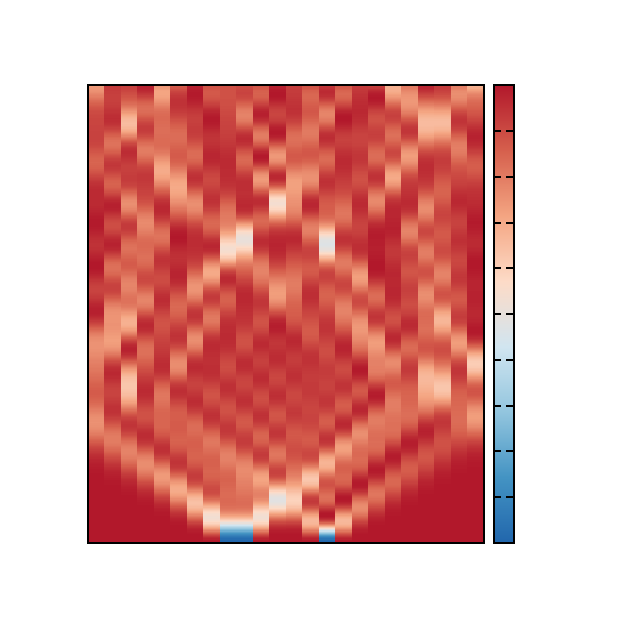
\includegraphics{SzCol_l0_mu0}}%
    \gplfronttext
  \end{picture}%
\endgroup
}
        \caption{$\mu=0$}
        \label{fig:testcollision1}
    \end{subfigure}
    \begin{subfigure}{.5\textwidth}
        \centering
        \resizebox{\textwidth}{!}{% GNUPLOT: LaTeX picture with Postscript
\begingroup
  \makeatletter
  \providecommand\color[2][]{%
    \GenericError{(gnuplot) \space\space\space\@spaces}{%
      Package color not loaded in conjunction with
      terminal option `colourtext'%
    }{See the gnuplot documentation for explanation.%
    }{Either use 'blacktext' in gnuplot or load the package
      color.sty in LaTeX.}%
    \renewcommand\color[2][]{}%
  }%
  \providecommand\includegraphics[2][]{%
    \GenericError{(gnuplot) \space\space\space\@spaces}{%
      Package graphicx or graphics not loaded%
    }{See the gnuplot documentation for explanation.%
    }{The gnuplot epslatex terminal needs graphicx.sty or graphics.sty.}%
    \renewcommand\includegraphics[2][]{}%
  }%
  \providecommand\rotatebox[2]{#2}%
  \@ifundefined{ifGPcolor}{%
    \newif\ifGPcolor
    \GPcolortrue
  }{}%
  \@ifundefined{ifGPblacktext}{%
    \newif\ifGPblacktext
    \GPblacktexttrue
  }{}%
  % define a \g@addto@macro without @ in the name:
  \let\gplgaddtomacro\g@addto@macro
  % define empty templates for all commands taking text:
  \gdef\gplbacktext{}%
  \gdef\gplfronttext{}%
  \makeatother
  \ifGPblacktext
    % no textcolor at all
    \def\colorrgb#1{}%
    \def\colorgray#1{}%
  \else
    % gray or color?
    \ifGPcolor
      \def\colorrgb#1{\color[rgb]{#1}}%
      \def\colorgray#1{\color[gray]{#1}}%
      \expandafter\def\csname LTw\endcsname{\color{white}}%
      \expandafter\def\csname LTb\endcsname{\color{black}}%
      \expandafter\def\csname LTa\endcsname{\color{black}}%
      \expandafter\def\csname LT0\endcsname{\color[rgb]{1,0,0}}%
      \expandafter\def\csname LT1\endcsname{\color[rgb]{0,1,0}}%
      \expandafter\def\csname LT2\endcsname{\color[rgb]{0,0,1}}%
      \expandafter\def\csname LT3\endcsname{\color[rgb]{1,0,1}}%
      \expandafter\def\csname LT4\endcsname{\color[rgb]{0,1,1}}%
      \expandafter\def\csname LT5\endcsname{\color[rgb]{1,1,0}}%
      \expandafter\def\csname LT6\endcsname{\color[rgb]{0,0,0}}%
      \expandafter\def\csname LT7\endcsname{\color[rgb]{1,0.3,0}}%
      \expandafter\def\csname LT8\endcsname{\color[rgb]{0.5,0.5,0.5}}%
    \else
      % gray
      \def\colorrgb#1{\color{black}}%
      \def\colorgray#1{\color[gray]{#1}}%
      \expandafter\def\csname LTw\endcsname{\color{white}}%
      \expandafter\def\csname LTb\endcsname{\color{black}}%
      \expandafter\def\csname LTa\endcsname{\color{black}}%
      \expandafter\def\csname LT0\endcsname{\color{black}}%
      \expandafter\def\csname LT1\endcsname{\color{black}}%
      \expandafter\def\csname LT2\endcsname{\color{black}}%
      \expandafter\def\csname LT3\endcsname{\color{black}}%
      \expandafter\def\csname LT4\endcsname{\color{black}}%
      \expandafter\def\csname LT5\endcsname{\color{black}}%
      \expandafter\def\csname LT6\endcsname{\color{black}}%
      \expandafter\def\csname LT7\endcsname{\color{black}}%
      \expandafter\def\csname LT8\endcsname{\color{black}}%
    \fi
  \fi
    \setlength{\unitlength}{0.0500bp}%
    \ifx\gptboxheight\undefined%
      \newlength{\gptboxheight}%
      \newlength{\gptboxwidth}%
      \newsavebox{\gptboxtext}%
    \fi%
    \setlength{\fboxrule}{0.5pt}%
    \setlength{\fboxsep}{1pt}%
\begin{picture}(5760.00,5760.00)%
    \gplgaddtomacro\gplbacktext{%
      \csname LTb\endcsname%
      \put(550,709){\makebox(0,0)[r]{\strut{}$0$}}%
      \put(550,1257){\makebox(0,0)[r]{\strut{}$1$}}%
      \put(550,1805){\makebox(0,0)[r]{\strut{}$2$}}%
      \put(550,2353){\makebox(0,0)[r]{\strut{}$3$}}%
      \put(550,2902){\makebox(0,0)[r]{\strut{}$4$}}%
      \put(550,3450){\makebox(0,0)[r]{\strut{}$5$}}%
      \put(550,3998){\makebox(0,0)[r]{\strut{}$6$}}%
      \put(550,4546){\makebox(0,0)[r]{\strut{}$7$}}%
      \put(550,5094){\makebox(0,0)[r]{\strut{}$8$}}%
      \put(761,484){\makebox(0,0){\strut{}$0$}}%
      \put(1554,484){\makebox(0,0){\strut{}$5$}}%
      \put(2346,484){\makebox(0,0){\strut{}$10$}}%
      \put(3138,484){\makebox(0,0){\strut{}$15$}}%
      \put(3930,484){\makebox(0,0){\strut{}$20$}}%
    }%
    \gplgaddtomacro\gplfronttext{%
      \csname LTb\endcsname%
      \put(176,2901){\rotatebox{-270}{\makebox(0,0){\strut{}time $t$}}}%
      \put(2583,154){\makebox(0,0){\strut{}particle index $i$}}%
      \put(2583,5429){\makebox(0,0){\strut{}$\lambda=0,~\mu=$5.}}%
      \csname LTb\endcsname%
      \put(4902,704){\makebox(0,0)[l]{\strut{}$-0.5$}}%
      \put(4902,1143){\makebox(0,0)[l]{\strut{}$-0.4$}}%
      \put(4902,1583){\makebox(0,0)[l]{\strut{}$-0.3$}}%
      \put(4902,2022){\makebox(0,0)[l]{\strut{}$-0.2$}}%
      \put(4902,2462){\makebox(0,0)[l]{\strut{}$-0.1$}}%
      \put(4902,2901){\makebox(0,0)[l]{\strut{}$0$}}%
      \put(4902,3341){\makebox(0,0)[l]{\strut{}$0.1$}}%
      \put(4902,3780){\makebox(0,0)[l]{\strut{}$0.2$}}%
      \put(4902,4220){\makebox(0,0)[l]{\strut{}$0.3$}}%
      \put(4902,4659){\makebox(0,0)[l]{\strut{}$0.4$}}%
      \put(4902,5099){\makebox(0,0)[l]{\strut{}$0.5$}}%
      \put(5496,2901){\rotatebox{-270}{\makebox(0,0){\strut{}$\braket{S_1^z}_t$}}}%
    }%
    \gplbacktext
    \put(0,0){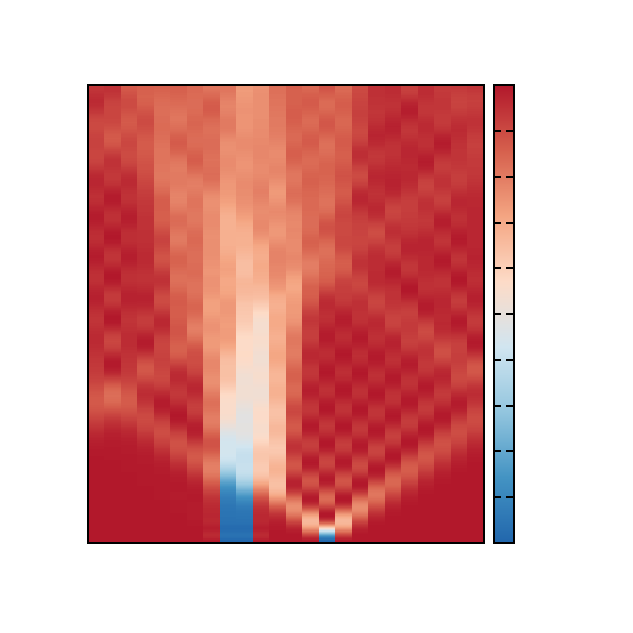
\includegraphics{SzCol_l0_mu5}}%
    \gplfronttext
  \end{picture}%
\endgroup
}
        \caption{$\mu=0$}
        \label{fig:testcollision2}
    \end{subfigure}
    \caption{d}
\end{figure}
\chapter{Ergebnisse}
Test\dots
citation: \cite{sand11}
F5 - Test:\\
\begin{align}
    \bra{\Psi}\ket{\Phi}
    \label{H}
\end{align}
in \cref{H} wird\dots
$\braket{8|s|7|6}$\\

\textbf{Griechische Buchstaben:}\\
\begin{align}
    \alpha\beta\chi\delta\varepsilon\varphi\gamma\eta\iota\kappa\lambda\mu\nu\pi\theta\rho\sigma\tau\upsilon\varsigma\xi\psi\zeta\\
    \Delta\Phi\Gamma\Lambda\Xi\Psi\Sigma\Upsilon\Omega\label{1}\\
    \braket{\Psi|\hat{H}|\Psi}\\\label{2}\\
    \vect{V}=\vec{V}\\
\end{align}
Label \cref{1,2}

$(\partial_\mu\partial^\mu+m^2)\Psi=0$\\
$\frac{5}{8}=z$\\
$A\circ B$\\
$A\equiv B$
\begin{align}
    \setminus\bigcap\times\wedge\bigcap\bigcup\subset\supset\le\ge\nonumber\dot{A}\ddot{B}\sqrt{A}\Big|\int_{-\infty}^{\infty}\d x  
    \label{b}
\end{align}

\begin{align}
    \partial_\mu F^{\mu\nu}&=\mu_0 j^\nu\\
    \partial_\mu \tilde{F}^{\mu\nu}&=0
\end{align}
\chapter{Diskussion}
Text\dots
\section{Unterkapitel}
Text\dots
\subsection{Unterkapitel}
Text\dots

\chapter{Zusammenfassung}
Text\dots

\appendix
\chapter{Calculation of $[S_i^z,H]=0$}

\chapter{zweiter Anhang}
Text\dots

\cleardoublepage
%% Bibliographie. Das Argument muss der Name der BIBTeX-Datenbank stehen.
%% Ein Beispiel fuer eine solche Datenbank finden Sie in bthesis_datenbank.bib
\bibliography{bthesis_datenbank} 

\chapter*{Danksagung}
Dank\dots

%% Dieser Befehl MUSS am Ende stehen und erzeugt die Erklaerung ueber die
%% benutzten Mittel
\Declaration
\end{document}
